\documentclass[12pt]{book} 
\usepackage{times}
\usepackage{amsmath}
\usepackage{epsfig}
\setlength{\oddsidemargin}{0.0in}
\setlength{\evensidemargin}{0.0in}
\setlength{\topmargin}{0.0in}
\setlength{\textheight}{9.0in}
\setlength{\textwidth}{6.5in}
\parindent=0.0pt
\parskip=14pt
%\baselineskip=14pt
%\renewcommand{\chaptername}{Lab}
\newcommand{\clearemptydoublepage}{\newpage{\pagestyle{empty}\cleardoublepage}}
\begin{document}
\title{Research notes for the multiband FLEX code with ODLRO}
\author{John Deisz}
\maketitle

\parskip=0pt
\tableofcontents
\parskip=14pt

\chapter{Hubbard Hamiltonian}
\label{chapter:hubbard}

\section{Normal terms}
\label{section:hubbard-normal}
The Hamiltonian for the Hubbard model is defined as 
\begin{equation}
\begin{split}
H - \mu N &= -\sum_{<\mathbf{r},\mathbf{r}^{\prime}>,\nu\nu^{\prime}\sigma}  
\left(t_{\nu\nu^{\prime}}(\mathbf{r},\mathbf{r}^{\prime})
e^{i \vec{\chi}\cdot (\mathbf{r}-\mathbf{r}^{\prime})}  
c^{\dagger}_{\vec{r}\nu\sigma}c_{\vec{r}^{\prime}\nu^{\prime}\sigma} + 
\mathrm{h.c.} \right) \\
& - \sum_{\mathbf{r}\nu\sigma} \mu \; c^{\dagger}_{\mathbf{r}\nu\sigma}c_{\vec{r}\nu\sigma} 
 -\sum_{\mathbf{r}\nu\sigma\sigma^{\prime}} \mathbf{h}\cdot 
\vec{\sigma}_{\sigma\sigma^{\prime}} 
\, c^{\dagger}_{\vec{r}\nu\sigma} c_{\vec{r}\nu\sigma^{\prime}} \\
& + \sum_{\mathbf{r}\nu\nu^{\prime}\sigma\sigma^{\prime}} U_{\nu\nu^{\prime}} 
c^{\dagger}_{\mathbf{r}\nu\sigma}c_{\mathbf{r}\nu\sigma}
c^{\dagger}_{\mathbf{r}\nu^{\prime}\sigma^{\prime}}c_{\mathbf{r}\nu^{\prime}\sigma^{\prime}} 
+ \sum_{\mathbf{r}\nu\nu^{\prime}\sigma\sigma^{\prime}} J_{\nu\nu^{\prime}}
c^{\dagger}_{\mathbf{r}\nu\sigma}c_{\mathbf{r}\nu^{\prime}\sigma^{\prime}}
c^{\dagger}_{\mathbf{r}\nu^{\prime}\sigma^{\prime}}c_{\mathbf{r}\nu\sigma}
\end{split}
\end{equation}
Along with the hopping amplitude, 
$t_{\nu\nu^{\prime}}(\mathbf{r},\mathbf{r}^{\prime})$, 
we include a phase factor with a term
$\vec{\chi}\cdot(\mathbf{r}-\mathbf{r}^{\prime}) 
\equiv 2 \pi (\phi_{B,x} / \phi_o)( (x-x^{\prime})/ L_x)$
+ similar terms for the $y$ and $z$ directions.
This phase factor characterizes the Aharanov-Bohm
phase acqured when an electron makes one complete revolution
around the lattice in the $x$, $y$ or
$z$ directions and, in doing
so, completes a circuit that encloses a magnetic
flux, $\phi_{B,x}$, $\phi_{B,y}$ and/or $\phi_{B,z}$. 

The chemical potential, $\mu$, regulates the number of
electrons in the system.  A uniform magnetic field, $\mathbf{h}$,
polarizes the electron spin.
Direct coulomb, $U$, and exchange terms, $J$, characterize the 
effective interaction between electrons on the same atomic site.

The transformation from ${\mathbf k}$-space to ${\mathbf r}$-space
is made by subsituting 
\begin{eqnarray}
\label{c-forward}
c^{\dagger}_{{\mathbf k}\nu\sigma} & = & \frac{1}{\sqrt{N}}
\sum_{{\mathbf r}} \exp(i \mathbf{k}\cdot\mathbf{r}) \; 
c^{\dagger}_{{\mathbf r}\nu\sigma} \\
\label{c-backwards}
c^{\dagger}_{{\mathbf r}\nu\sigma} & = & \frac{1}{\sqrt{N}}
\sum_{{\mathbf k}} \exp(-i \mathbf{k}\cdot\mathbf{r}) \; 
c^{\dagger}_{{\mathbf k}\nu\sigma} 
\end{eqnarray}
with equivalent relations for the annihilation operators
obtained by taking the 
Hermetian conjugates of Eqs~(\ref{c-forward}) and (\ref{c-backwards}).
Local terms transform as follows:
\begin{eqnarray}
\sum_{\mathbf{r}} c^{\dagger}_{\mathbf{r}\nu\sigma} c_{\mathbf{r}\nu\sigma} & = &
\frac{1}{N} \sum_{\mathbf{r}} \sum_{\mathbf{k},\mathbf{k}^{\prime}}
e^{-i \mathbf{k}\cdot\mathbf{r}} e^{i \mathbf{k}^{\prime}\cdot\mathbf{r}}
c^{\dagger}_{\mathbf{k}\nu\sigma} c_{\mathbf{k}^{\prime}\nu\sigma} \\
& = & \sum_{\mathbf{k},\mathbf{k}^{\prime}} 
\delta_{\mathbf{k},\mathbf{k}^{\prime}}
c^{\dagger}_{\mathbf{k}\nu\sigma} c_{\mathbf{k}^{\prime}\nu\sigma} \\
& = & \sum_{\mathbf{k}} c^{\dagger}_{\mathbf{k}\nu\sigma} c_{\mathbf{k}\nu\sigma}
\end{eqnarray}  
Likewise we obtain a simple form for the kinetic energy terms
when they are expressed in momentum space:
\begin{eqnarray}
\mathrm{KE} & = &
-\sum_{<\mathbf{r}\mathbf{r}^{\prime}>\nu\nu^{\prime}\sigma} 
t_{\nu\nu^{\prime}}(\mathbf{r},\mathbf{r}^{\prime})
e^{i\vec{\chi}\cdot(\mathbf{r}-\mathbf{r}^{\prime})}
c^{\dagger}_{\mathbf{r}\nu\sigma}c_{\mathbf{r}^{\prime}\nu^{\prime}\sigma} + 
 t_{\nu\nu^{\prime}}^*(\mathbf{r},\mathbf{r}^{\prime}) 
e^{-i\vec{\chi}\cdot (\mathbf{r}-\mathbf{r}^{\prime})}
c^{\dagger}_{\mathbf{r}^{\prime}\nu^{\prime}\sigma}c_{\mathbf{r}\nu\sigma} \\
& = & -\sum_{<\mathbf{r}\mathbf{r}^{\prime}>\nu\nu^{\prime}\sigma} 
t_{\nu\nu^{\prime}}(\mathbf{r},\mathbf{r}^{\prime})
e^{i\vec{\chi}\cdot(\mathbf{r}-\mathbf{r}^{\prime})}
c^{\dagger}_{\mathbf{r}\nu\sigma}c_{\mathbf{r}^{\prime}\nu^{\prime}\sigma} +
 t_{\nu^{\prime}\nu}^*(\mathbf{r}^{\prime},\mathbf{r})
e^{-i\vec{\chi}\cdot(\mathbf{r}^{\prime}-\mathbf{r})}
c^{\dagger}_{\mathbf{r}\nu\sigma}c_{\mathbf{r}^{\prime}\nu^{\prime}\sigma} \\
& = & -\frac{1}{2} \sum_{\mathbf{r}^{\prime}\vec{\delta}\nu\nu^{\prime}\sigma} 
t_{\nu\nu^{\prime}}(\vec{\delta}) e^{i\vec{\chi}\cdot \vec{\delta}} 
c^{\dagger}_{\mathbf{r}^{\prime}+\vec{\delta}\nu\sigma} c_{\vec{r}^{\prime}\nu^{\prime}\sigma}
+ t_{\nu^{\prime}\nu}^*(-\vec{\delta}) e^{ i \vec{\chi} \cdot \vec{\delta}} 
c^{\dagger}_{\mathbf{r}^{\prime}+ \vec{\delta}\nu\sigma} c_{\mathbf{r}^{\prime}\nu^{\prime}\sigma} \\
& = & - \sum_{\mathbf{r}^{\prime}\vec{\delta}} t_{\nu\nu^{\prime}}(\vec{\delta}) 
e^{i \vec{\chi}\cdot \vec{\delta}} 
c^{\dagger}_{\mathbf{r}^{\prime}+\vec{\delta}\nu\sigma} c_{\vec{r}^{\prime}\nu^{\prime}\sigma}
\end{eqnarray}
since $t_{\nu^{\prime}\nu}^*(-\vec{\delta}) = t_{\nu\nu^{\prime}}(\vec{\delta})$.
Substituation of Eq.~(\ref{c-backwards}) gives
\begin{eqnarray}
& = &-\frac{1}{N}
\sum_{\mathbf{r}\vec{\delta}\nu\nu^{\prime}\sigma \mathbf{k}\mathbf{k}^{\prime}}
t_{\nu\nu^{\prime}}(\vec{\delta})e^{i\vec{\chi}\cdot \vec{\delta}} 
e^{-i \mathbf{k}\cdot (\mathbf{r} + \vec{\delta})}
e^{i \mathbf{k}^{\prime} \cdot \mathbf{r}}
     c^{\dagger}_{\mathbf{k}\nu\sigma}
  c_{\mathbf{k}^{\prime}\nu^{\prime}\sigma} \\
& = & - \sum_{\vec{\delta}\nu\nu^{\prime}\mathbf{k},\mathbf{k}^{\prime}}
t_{\nu\nu^{\prime}}(\vec{\delta})e^{i \vec{\chi}\cdot \vec{\delta}} 
 e^{-i \mathbf{k}\cdot \vec{\delta}} \delta_{\mathbf{k},\mathbf{k}^{\prime}}
     c^{\dagger}_{\mathbf{k}\nu\sigma}
  c_{\mathbf{k}^{\prime}\nu^{\prime}\sigma} \\
& = & - \sum_{\mathbf{k}\vec{\delta}\nu\nu^{\prime}}  
e^{-i \mathbf{k}\cdot \vec{\delta}} 
t_{\nu\nu^{\prime}}(\vec{\delta})e^{i \vec{\chi}\cdot\vec{\delta}} 
  c^{\dagger}_{\mathbf{k}\nu\sigma}
  c_{\mathbf{k}\nu^{\prime}\sigma} \\
& = & \sum_{\mathbf{k}\nu\nu^{\prime}} \epsilon_{\nu\nu^{\prime}}(\mathbf{k})
  c^{\dagger}_{\mathbf{k}\nu\sigma}
  c_{\mathbf{k}\nu^{\prime}\sigma}
 \end{eqnarray}
where
\begin{equation}
\epsilon_{\nu\nu^{\prime}}(\mathbf{k}) = - \sum_{\vec{\delta}} 
e^{-i \mathbf{k}\cdot\vec{\delta}} e^{i \vec{\chi}\cdot\vec{\delta}}  
t_{\nu\nu^{\prime}}(\vec{\delta})
\end{equation}
is the Fourier transform of the hopping integrals.
Thus, if we write all the one-electron terms in $\mathbf{k}$-space
the Hamiltonian becomes
\begin{equation}
H_0 - \mu N =  \sum_{\mathbf{k}\nu\nu^{\prime}\sigma\sigma^{\prime}} 
((\epsilon_{\nu\nu^{\prime}}(\mathbf{k}) - \mu\delta_{\nu\nu^{\prime}})
\delta_{\sigma\sigma^{\prime}} -
 \mathbf{h}\cdot\vec{\sigma}_{\sigma\sigma^{\prime}}\delta_{\nu\nu^{\prime}}) 
c^{\dagger}_{\mathbf{k}\nu\sigma}
 c_{\mathbf{k}\nu^{\prime}\sigma^{\prime}} 
\end{equation} 

\section{External pair-field coupling terms}
\label{section:pair-field}

Let
\begin{eqnarray}
H_{p} & = & - \frac{\sqrt{N_l}}{2} 
\sum_{\mathbf{r}\mathbf{r}^{\prime}\nu\nu^{\prime}\sigma\sigma^{\prime}} 
h_p \left( \Psi_{\nu\sigma\nu^{\prime}\sigma^{\prime}}(\mathbf{r},\mathbf{r}^{\prime})
c_{\mathbf{r}\nu\sigma}
c_{\mathbf{r}^{\prime}\nu^{\prime}\sigma^{\prime}} + \mathrm{h.c.}\right) \\
 &  = & - \frac{\sqrt{N_l}}{2} \sum_{\mathbf{r}\mathbf{r}^{\prime}\nu\nu^{\prime}\sigma\sigma^{\prime}} 
h_p \left(\Psi_{\nu\sigma\nu^{\prime}\sigma^{\prime}}(\mathbf{r},\mathbf{r}^{\prime})  
c_{\mathbf{r}\nu\sigma}
c_{\mathbf{r}^{\prime}\nu^{\prime}\sigma^{\prime}} + 
\Psi_{\nu\sigma\nu^{\prime}\sigma^{\prime}}^*(\mathbf{r},\mathbf{r}^{\prime}) 
c^{\dagger}_{\mathbf{r}^{\prime}\nu^{\prime}\sigma^{\prime}}
 c^{\dagger}_{\mathbf{r}\nu\sigma}\right) \\
& = &  - \frac{\sqrt{N_l}}{2} 
\sum_{\mathbf{r}\mathbf{r}^{\prime}\nu\nu^{\prime}\sigma\sigma^{\prime}} 
h_p \left(\Psi_{\nu\sigma\nu^{\prime}\sigma^{\prime}}(\mathbf{r},\mathbf{r}^{\prime})  
c_{\mathbf{r}\nu\sigma}
c_{\mathbf{r}^{\prime}\nu^{\prime}\sigma^{\prime}} + 
\Psi_{\nu^{\prime}\sigma^{\prime}\nu\sigma}^*(\mathbf{r}^{\prime},\mathbf{r}) 
 c^{\dagger}_{\mathbf{r}\nu\sigma}c^{\dagger}_{\mathbf{r}^{\prime}\nu^{\prime}\sigma^{\prime}}
  \right)
\end{eqnarray}
Here $\Psi$ is the normalized pairing wave function
where the normalization is given by
\begin{equation}
\sum_{\mathbf{r}\mathbf{r}^{\prime}\nu\nu^{\prime}\sigma\sigma^{\prime}} | 
\Psi_{\nu\sigma\nu^{\prime}\sigma^{\prime}}(\mathbf{r},\mathbf{r}^{\prime}) |^2 = 1,
\end{equation}
$N_l$ is the number of lattice points
and the real constant $h_p$ describes the strength of the
pairing field.

Since 
$\{c_{\mathbf{r}\nu\sigma},c_{\mathbf{r}^{\prime}\nu^{\prime}\sigma^{\prime}}\}=0$ by the Fermi
commutation relations, only the antisymmetric part of
$\Psi$ effectively contributes to this term.
Forcing $\Psi$ to be antisymmetric gives us
$\Psi_{\nu^{\prime}\sigma^{\prime}\nu\sigma}(\mathbf{r}^{\prime},\mathbf{r}) =
- \Psi_{\nu\sigma\nu^{\prime}\sigma^{\prime}}(\mathbf{r},\mathbf{r}^{\prime})$.
Other than this,
the functional dependence of $\Psi$ may be arbitary, but we
will be interested in forms for $\Psi$ that represent
the dominant pairing symmetry for this model.  When there is
translational invariance we expect that
\begin{equation}
 | \Psi_{\nu\sigma\nu^{\prime}\sigma^{\prime}}(\mathbf{r}+\vec{\delta},
\mathbf{r}^{\prime}+\vec{\delta}) | =
|\Psi_{\nu\sigma\nu^{\prime}\sigma^{\prime}}(\mathbf{r},\mathbf{r}^{\prime})|
\end{equation}
so that
\begin{equation}
\Psi_{\nu\sigma\nu^{\prime}\sigma^{\prime}}(\mathbf{r}+\vec{\delta},
\mathbf{r}^{\prime}+\vec{\delta}) = 
e^{i\theta(\vec{\delta})} 
\Psi_{\nu\sigma\nu^{\prime}\sigma^{\prime}}(\mathbf{r},\mathbf{r}^{\prime}).
\end{equation}
(\textbf{Note: does $\theta$ need to have band and spin indices?'})
Since the pairing field must be single valued we require 
$\Psi_{\nu\sigma\nu^{\prime}\sigma^{\prime}}(\vec{r} + L_x\hat{x}, \vec{r}^{\prime} + L_x \hat{x}) = 
\Psi_{\nu\sigma\nu^{\prime}\sigma^{\prime}}(\vec{r}, \vec{r}^{\prime})$
with similar relations for center-of-mass displacements in the 
$y$ and $z$ directions.
We assume also that the spatial variation of the phase will
be as smooth as possible.  This leads to
\begin{equation}
\theta(\vec{\delta}) = 2 \pi (n_{p,x} \delta_x / L_x + n_{p,y} 
\delta_y / L_y
+ n_{p,z} \delta_z / L_z).
\end{equation}
$n_{p,x}$ is an integer that describes the number times
the phase rotates for each $\delta_x = L_x$ of displacement
and has only $L_x$ unique values which we take to be
given by $n_{p,x} = -L_x/2 + 1, -L_x/2 + 2, \cdots -1, 0, 1, \cdots L_x/2$.

Based on these considerations we write
\begin{equation}
\Psi_{\nu\sigma\nu^{\prime}\sigma^{\prime}}(\mathbf{r},\mathbf{r}^{\prime}) = 
\psi\left(\mathbf{r}_{cm}\right) 
\phi_{\nu\sigma\nu^{\prime}\sigma^{\prime}}(\mathbf{r} - \mathbf{r}^{\prime}).
\end{equation}
where the center of mass part, $\psi(\mathbf{r}_{cm})$, is given
by
\begin{equation}
\psi(\mathbf{r}_{cm}) = 
\frac{1}{\sqrt{N_l}}e^{i 2 \pi ( n_{p,x} x_{cm} / L_x + n_{p,y} y_{cm}/L_y + 
n_{p,z} z_{cm}/L_z)}
\end{equation}
and the normalization of $\phi$ is given by
\begin{eqnarray}
\sum_{\mathbf{r}\mathbf{r}^{\prime}\nu\nu^{\prime}\sigma\sigma^{\prime}} 
|\Psi_{\nu\sigma\nu^{\prime}\sigma^{\prime}}(\mathbf{r},\mathbf{r}^{\prime})|^2 
& = & 1 \\
\frac{1}{N_l}
\sum_{\mathbf{r}\mathbf{r}^{\prime}\nu\nu^{\prime}\sigma\sigma^{\prime}} 
|\phi_{\nu\sigma\nu^{\prime}\sigma^{\prime}}(\mathbf{r} - \mathbf{r}^{\prime}) |^2 
& = & 1\\
\frac{1}{N_l} N_l \sum_{\vec{\delta}\nu\nu^{\prime}\sigma\sigma^{\prime}} 
|\phi_{\nu\sigma\nu^{\prime}\sigma^{\prime}}(\vec{\delta})|^2 & = & 
1 \\
\sum_{\vec{\delta}\nu\nu^{\prime}\sigma\sigma^{\prime}} 
|\phi_{\nu\sigma\nu^{\prime}\sigma^{\prime}}(\vec{\delta}) |^2 & = & 1.
\end{eqnarray}
Thus, the final real-space form for $H_p$ is given (in conventional
notation) by
\begin{equation}
\label{H_p_real}
H_p = -\frac{1}{2}
\sum_{\mathbf{r}\mathbf{r}^{\prime}\nu\nu^{\prime}\sigma\sigma^{\prime}} 
 h_p \left(e^{i 2 \pi \vec{n_p}\cdot \vec{r}_{cm}/L} 
\phi_{\nu\sigma\nu^{\prime}\sigma^{\prime}}(\mathbf{r} -
\mathbf{r}^{\prime}) c_{\mathbf{r}\nu\sigma} c_{\mathbf{r}\nu^{\prime}\sigma^{\prime}}
+e^{-i 2 \pi \vec{n_p}\cdot \vec{r}_{cm}/L} 
\phi_{\nu^{\prime}\sigma^{\prime}\nu\sigma}^*(\mathbf{r}^{\prime} -
\mathbf{r})c^{\dagger}_{\mathbf{r}\nu\sigma}
c^{\dagger}_{\mathbf{r}^{\prime}\nu^{\prime}\sigma^{\prime}} \right).
\end{equation}

Next we convert $H_p$ to $\mathbf{k}$-space.  After substituting
using Eq.~(\ref{c-backwards}) we get
\begin{equation}
\begin{split}
H_p = & - \frac{h_p}{2N} \sum_{\mathbf{r}\mathbf{r}^{\prime}\sigma\sigma^{\prime}} 
\sum_{\mathbf{k},\mathbf{k}^{\prime}}
e^{i 2 \pi \vec{n_p}\cdot \vec{r}_{cm}/L}
\phi_{\nu\sigma\nu^{\prime}\sigma^{\prime}}(\mathbf{r} - \mathbf{r}^{\prime})
c_{\mathbf{k}\nu\sigma} c_{\mathbf{k}^{\prime}\nu^{\prime}\sigma^{\prime}}
e^{i \mathbf{k}\cdot\mathbf{r}} e^{i \mathbf{k}^{\prime}\cdot
\mathbf{r}^{\prime}} 
\\
& + e^{-i 2 \pi \vec{n_p}\cdot \vec{r}_{cm}/L} 
\phi_{\nu^{\prime}\sigma^{\prime}\nu\sigma}^*(\mathbf{r}^{\prime} - \mathbf{r})
 c^{\dagger}_{\mathbf{k}^{\prime}\nu\sigma}
 c^{\dagger}_{\mathbf{k}\nu^{\prime}\sigma^{\prime}} 
e^{-i\mathbf{k}^{\prime}\cdot\mathbf{r}}
 e^{-i \mathbf{k}\cdot \mathbf{r}^{\prime}}  \\
 = & -\frac{h_p}{2N} 
 \sum_{\mathbf{k}\mathbf{k}^{\prime}}
 \sum_{\mathbf{r}_{cm} \vec{\delta}\nu\nu^{\prime}\sigma\sigma^{\prime}}
e^{i 2 \pi \vec{n_p}\cdot \vec{r}_{cm}/L} 
\phi_{\nu\sigma\nu^{\prime}\sigma^{\prime}}(\vec{\delta})\,
 c_{\mathbf{k}\nu\sigma} c_{\mathbf{k}^{\prime}\nu^{\prime}\sigma^{\prime}}
 e^{i(\mathbf{k}-\mathbf{k}^{\prime})/\cdot \vec{\delta}/2} 
 e^{i (\mathbf{k}^{\prime}+\mathbf{k})\cdot \mathbf{r}_{cm}}  \\
 & 
 -\frac{h_p}{2N} 
 \sum_{\mathbf{k}\mathbf{k}^{\prime}}
 \sum_{\mathbf{r}_{cm}\vec{\delta}\nu\nu^{\prime}\sigma\sigma^{\prime}} 
  e^{-i 2 \pi \vec{n_p}\cdot \vec{r}_{cm}/L}
\phi_{\nu^{\prime}\sigma^{\prime}\nu\sigma}^*(\vec{\delta})
 c^{\dagger}_{\mathbf{k}^{\prime}\nu\sigma}
 c^{\dagger}_{\mathbf{k}\nu^{\prime}\sigma^{\prime}}
 e^{-i(\mathbf{k}+\mathbf{k}^{\prime})\cdot \mathbf{r}_{cm}}
 e^{-i(\mathbf{k}-\mathbf{k}^{\prime})\cdot\vec{\delta}/2}  \\
= & -\frac{h_p}{2}
\sum_{\mathbf{k}\mathbf{k}^{\prime}\vec{\delta}\nu\nu^{\prime}\sigma\sigma^{\prime}}
\phi_{\nu\sigma\nu^{\prime}\sigma^{\prime}}(\vec{\delta}) c_{\mathbf{k}\nu\sigma}
c_{\mathbf{k}^{\prime}\nu^{\prime}\sigma^{\prime}} 
e^{i(\mathbf{k}-\mathbf{k}^{\prime})\cdot\vec{\delta}}
\delta_{\mathbf{k}^{\prime},-\mathbf{k}- 2 \pi \vec{n}_p /L} \\
& + \phi_{\nu^{\prime}\sigma^{\prime}\nu\sigma}^*(\vec{\delta})
c^{\dagger}_{\mathbf{k}^{\prime}\nu\sigma}
c_{\mathbf{k}\nu^{\prime}\sigma^{\prime}} 
e^{-i (\mathbf{k}-\mathbf{k}^{\prime})\cdot\vec{\delta}}
\delta_{\mathbf{k}^{\prime},-\mathbf{k} - 2\pi \vec{n}_p /L_x}  \\
= & - \frac{h_p}{2} \sum_{\mathbf{k}\vec{\delta}\nu\nu^{\prime}\sigma\sigma^{\prime}}
\phi_{\nu\sigma\nu^{\prime}\sigma^{\prime}}(\vec{\delta})
e^{i (\mathbf{k}+ \pi\vec{n}_p/L)\cdot \vec{\delta}}
c_{\mathbf{k}\nu\sigma} 
c_{-\mathbf{k} - 2 \pi \vec{n}_p / L,\nu^{\prime}\sigma^{\prime}} \\
& + \phi_{\nu^{\prime}\sigma^{\prime}\nu\sigma}^*(\vec{\delta})
e^{-i (\mathbf{k}+ \pi\vec{n}_p/L)\cdot \vec{\delta}}  
c^{\dagger}_{-\mathbf{k} -2 \pi \vec{n}_p / L,\nu\sigma}
c^{\dagger}_{\mathbf{k}\nu^{\prime}\sigma^{\prime}}.
\end{split}
\end{equation}
If we set
\begin{equation}
\phi_{\nu\sigma\nu^{\prime}\sigma^{\prime}}(\mathbf{k}) \equiv \sum_{\vec{\delta}}
e^{-i \mathbf{k}\cdot\vec{\delta}}
\phi_{\nu\sigma\nu^{\prime}\sigma^{\prime}}(\vec{\delta}), 
\end{equation}
then we get
\begin{equation}
H_p = - \frac{h_p}{2} \sum_{\mathbf{k}\nu\nu^{\prime}\sigma\sigma^{\prime}} 
\phi_{\nu\sigma\nu^{\prime}\sigma^{\prime}}(-\mathbf{k}-\pi\vec{n}_p/L)
c_{\mathbf{k}\nu\sigma} 
c_{-\mathbf{k} - 2\pi \vec{n}_p/L,\nu^{\prime}\sigma^{\prime}}
+  \phi_{\nu^{\prime}\sigma^{\prime}\nu\sigma}^*(-\mathbf{k}-\pi\vec{n}_p/L)     
c^{\dagger}_{-\mathbf{k} - 2\pi\vec{n_p}/L\nu\sigma}
c_{\mathbf{k}\nu^{\prime}\sigma^{\prime}}.
\end{equation}

Thus, if $\vec{n}_p \neq 0$, then the electron pairs are
coupled such that their $x$-momenta differ by an amount equal
to $\pi \vec{n}_p/L$.  
For $|\phi_B| < \phi_o / 2$,
we expect $\vec{n}_p$ to be zero.  In that case, we
can write the final form of $H_p$ as
\begin{eqnarray}
H_p & = & - \frac{h_p}{2} \sum_{\mathbf{k}\nu\nu^{\prime}\sigma\sigma^{\prime}} 
\phi_{\nu\sigma\nu^{\prime}\sigma^{\prime}}(-\mathbf{k})
  c_{\mathbf{k}\nu\sigma}
  c_{-\mathbf{k}\nu^{\prime}\sigma^{\prime}}
+ \phi_{\nu^{\prime}\sigma^{\prime}\nu\sigma}^*(-\mathbf{k}) 
  c^{\dagger}_{-\mathbf{k}\nu\sigma}
  c^{\dagger}_{\mathbf{k}\nu^{\prime}\sigma^{\prime}}\\
 & = & - \frac{h_p}{2} \sum_{\mathbf{k}\nu\nu^{\prime}\sigma\sigma^{\prime}} 
\phi_{\nu\sigma\nu^{\prime}\sigma^{\prime}}(-\mathbf{k})
  c_{\mathbf{k}\nu\sigma}
  c_{-\mathbf{k}\nu^{\prime}\sigma^{\prime}}
+ \phi_{\nu^{\prime}\sigma^{\prime}\nu\sigma}^*(\mathbf{k}) 
  c^{\dagger}_{\mathbf{k}\nu\sigma}
  c^{\dagger}_{-\mathbf{k}\nu^{\prime}\sigma^{\prime}}
\end{eqnarray}



\chapter{Nambu formalism and the non-interacting Green's function}
\label{chapter:g0}

\section{Definitions}

To account for broken U(1) symmetry in the Green's function, we
introduce the Nambu representation for the field operator, $\psi$, as
\begin{eqnarray}
\psi_{\mathbf{r}\nu 0} & = & c_{\mathbf{r}\nu\uparrow} \\
\psi_{\mathbf{r}\nu 1} & = & c_{\mathbf{r}\nu\downarrow} \\
\psi_{\mathbf{r}\nu 2} & = & c^{\dagger}_{\mathbf{r}\nu\uparrow} \\
\psi_{\mathbf{r}\nu 3} & = & c^{\dagger}_{\mathbf{r}\nu\downarrow} 
\end{eqnarray}
with Hermetian conjugates
\begin{eqnarray}
\psi^{\dagger}_{\mathbf{r}\nu 0} & = & c^{\dagger}_{\mathbf{r}\nu \uparrow} \\
\psi^{\dagger}_{\mathbf{r}\nu 1} & = & c^{\dagger}_{\mathbf{r}\nu \downarrow} \\
\psi^{\dagger}_{\mathbf{r}\nu 2} & = & c_{\mathbf{r}\nu \uparrow} \\
\psi^{\dagger}_{\mathbf{r}\nu 3} & = & c_{\mathbf{r}\nu \downarrow}. 
\end{eqnarray}
We treat these four components as corresponding to
four distinct particle types.  Of course, this
effectively double counts the number of degrees of freedom
and this must be accounted for in expressions for the
self-energy and
thermodynamic functions.

We define the momentum space operators via
\begin{equation}
\psi_{\mathbf{k}\nu\alpha} \equiv
\frac{1}{\sqrt{N}} 
\sum_{\mathbf{r}}
e^{-i \mathbf{k}\cdot \mathbf{r}} \psi_{\mathbf{r}\nu \alpha}
\end{equation}
so that
\begin{eqnarray}
\psi_{\mathbf{k}\nu 0} & = & c_{\mathbf{k}\nu\uparrow} \\
\psi_{\mathbf{k}\nu 1} & = & c_{\mathbf{k}\nu\downarrow} \\
\psi_{\mathbf{k}\nu 2} & = & c^{\dagger}_{-\mathbf{k}\nu\uparrow} \\
\psi_{\mathbf{k}\nu 3} & = & c^{\dagger}_{-\mathbf{k}\nu\downarrow}
\end{eqnarray}

The single-particle Green's function is defined as
\begin{equation}
G_{\nu\alpha\nu^{\prime}\alpha^{\prime}}(\mathbf{k},\tau) \equiv
- \cal{T}_{\tau} <\psi_{\mathbf{k}\nu\alpha}(\tau) 
\psi^{\dagger}_{\mathbf{k}\nu^{\prime}\alpha^{\prime}}>
\end{equation}
Although the momentum indices could be distinct in the
above, the Hamiltonian contains no terms that do not
obey momentum conservation when the Hamiltonian is
expressed properly in terms of $\psi$ and $\psi^{\dagger}$.
Thus, only the momentum diagonal form shown above is
non-zero.

\section{Evaluation of $G^{(0)}$}

We utilize the equation of motion technique to evaluate
the non-interacting Green's function, $G^{(0)}$.
In all cases, we have
\begin{equation}
\psi_{\mathbf{k}\nu\alpha}(\tau) \equiv
e^{(\hat{H}-\mu\hat{N})\tau} \psi_{\mathbf{k}\nu\alpha}
e^{-(\hat{H}-\mu\hat{N})\tau} 
\end{equation}
so that
\begin{eqnarray}
\frac{\partial \psi_{\mathbf{k}\nu\alpha}(\tau)}{\partial \tau} & = &
(\hat{H} - \mu \hat{N}) \psi_{\mathbf{k}\nu\alpha}(\tau) -
 \psi_{\alpha,\mathbf{k}}(\tau)(\hat{H} - \mu \hat{N}) \\
& = & \left[ (\hat{H} - \mu\hat{N}),\psi_{\mathbf{k}\nu\alpha}(\tau) \right]
\end{eqnarray}
In the absence of interactions we have
\begin{equation}
\begin{split}
\hat{H}^{(0)} - \mu \hat{N} = & \sum_{\mathbf{k}^{\prime}\nu^{\prime}\nu^{\prime\prime}\sigma^{\prime}}
 \xi_{\nu^{\prime}\nu^{\prime\prime}}(\mathbf{k}) 
c^{\dagger}_{\mathbf{k}^{\prime}\nu^{\prime}\sigma^{\prime}}
c_{\mathbf{k}^{\prime}\nu^{\prime\prime}\sigma^{\prime}} -
\sum_{\mathbf{k}^{\prime}\nu^{\prime}\sigma^{\prime}\sigma^{\prime\prime}}
\mathbf{h}\cdot\vec{\sigma}_{\sigma^{\prime}\sigma^{\prime\prime}}
c^{\dagger}_{\mathbf{k}^{\prime}\nu^{\prime}\sigma^{\prime}}
c_{\mathbf{k}^{\prime}\nu^{\prime}\sigma^{\prime\prime}} \\
& - \frac{h_p}{2}
\sum_{\mathbf{k}^{\prime}\nu^{\prime}\nu^{\prime\prime}\sigma^{\prime}\sigma^{\prime\prime}}
\left(\phi_{\nu^{\prime}\sigma^{\prime}\nu^{\prime\prime}\sigma^{\prime\prime}}(-\mathbf{k}^{\prime})
c_{\mathbf{k}^{\prime}\nu^{\prime}\sigma^{\prime}}
c_{-\mathbf{k}^{\prime}\nu^{\prime\prime}\sigma^{\prime\prime}}
+
\phi^*_{\nu^{\prime\prime}\sigma^{\prime\prime}\nu^{\prime}\sigma^{\prime}}(\mathbf{k}^{\prime})
c^{\dagger}_{\mathbf{k}^{\prime}\nu^{\prime}\sigma^{\prime}}
c^{\dagger}_{-\mathbf{k}^{\prime}\nu^{\prime\prime}\sigma^{\prime\prime}}\right)
\end{split}
\end{equation}
and these commutation relations are simple to evaluate.

For $\alpha = 0$ or 1 we have
\begin{equation}
\psi_{\mathbf{k}\nu\alpha}(\tau) = c_{\mathbf{k}\nu\sigma}(\tau).
\end{equation}
When we commute this with the hopping (and chemical potential) term in the
Hamiltonian we get
\begin{eqnarray}
& & 
\sum_{\mathbf{k}^{\prime}\nu^{\prime}\nu^{\prime\prime}\sigma^{\prime}} 
\xi_{\nu^{\prime}\nu^{\prime\prime}}(\mathbf{k}^{\prime})
\left[c^{\dagger}_{\mathbf{k}^{\prime}\nu^{\prime}\sigma^{\prime}}
c_{\mathbf{k}^{\prime}\nu^{\prime\prime}\sigma^{\prime}},
c_{\mathbf{k}\nu\sigma} \right] \\
& = & 
\sum_{\mathbf{k}^{\prime}\nu^{\prime}\nu^{\prime\prime}\sigma^{\prime}} 
\xi_{\nu^{\prime}\nu^{\prime\prime}}(\mathbf{k}^{\prime})
\left(c^{\dagger}_{\mathbf{k}^{\prime}\nu^{\prime}\sigma^{\prime}}
c_{\mathbf{k}^{\prime}\nu^{\prime\prime}\sigma^{\prime}}
c_{\mathbf{k}\nu\sigma} -
c_{\mathbf{k}\nu\sigma}
c^{\dagger}_{\mathbf{k}^{\prime}\nu^{\prime}\sigma^{\prime}}
c_{\mathbf{k}^{\prime}\nu^{\prime\prime}\sigma^{\prime}} \right)
\\
& = & 
\sum_{\mathbf{k}^{\prime}\nu^{\prime}\nu^{\prime\prime}\sigma^{\prime}} 
\xi_{\nu^{\prime}\nu^{\prime\prime}}(\mathbf{k}^{\prime})
\left(-c^{\dagger}_{\mathbf{k}^{\prime}\nu^{\prime}\sigma^{\prime}}
c_{\mathbf{k}\nu\sigma}
c_{\mathbf{k}^{\prime}\nu^{\prime\prime}\sigma^{\prime}} -
c_{\mathbf{k}\nu\sigma}
c^{\dagger}_{\mathbf{k}^{\prime}\nu^{\prime}\sigma^{\prime}}
c_{\mathbf{k}^{\prime}\nu^{\prime\prime}\sigma^{\prime}}
 \right) \\
& = & \sum_{\mathbf{k}^{\prime}\nu^{\prime}\nu^{\prime\prime}\sigma^{\prime}} 
\xi_{\nu^{\prime}\nu^{\prime\prime}}(\mathbf{k}^{\prime})
\left(-\delta_{\mathbf{k}^{\prime},\mathbf{k}}\delta_{\nu^{\prime}\nu}
\delta_{\sigma,\sigma^{\prime}}c_{\mathbf{k}^{\prime}\nu^{\prime\prime}\sigma^{\prime}}
\right) 
\\
& = & - \sum_{\nu^{\prime\prime}}\xi_{\nu\nu^{\prime\prime}}(\mathbf{k}) 
c_{\mathbf{k}\nu^{\prime\prime}\sigma}
\end{eqnarray}

The magnetic field term yields
\begin{eqnarray}
& & -\sum_{\mathbf{k}^{\prime}\nu^{\prime}\sigma^{\prime}
\sigma^{\prime\prime}}
\mathbf{h}\cdot \vec{\sigma}_{\sigma^{\prime}\sigma^{\prime\prime}}
\left[ c^{\dagger}_{\mathbf{k}^{\prime}\nu^{\prime}\sigma^{\prime}}
       c_{\mathbf{k}^{\prime}\nu^{\prime}\sigma^{\prime\prime}},
       c_{\mathbf{k}\nu\sigma} \right] \\
& &= -\sum_{\mathbf{k}^{\prime}\nu^{\prime}\sigma^{\prime}
\sigma^{\prime\prime}}
\mathbf{h}\cdot \vec{\sigma}_{\sigma^{\prime}\sigma^{\prime\prime}}
\left( c^{\dagger}_{\mathbf{k}^{\prime}\nu^{\prime}\sigma^{\prime}}
       c_{\mathbf{k}^{\prime}\nu^{\prime}\sigma^{\prime\prime}}
       c_{\mathbf{k}\nu\sigma} -
       c_{\mathbf{k}\nu\sigma}
 c^{\dagger}_{\mathbf{k}^{\prime}\nu^{\prime}\sigma^{\prime}}
       c_{\mathbf{k}^{\prime}\nu^{\prime}\sigma^{\prime\prime}}\right) \\
& &= -\sum_{\mathbf{k}^{\prime}\nu^{\prime}\sigma^{\prime}
\sigma^{\prime\prime}}
\mathbf{h}\cdot \vec{\sigma}_{\sigma^{\prime}\sigma^{\prime\prime}}
\left(- c^{\dagger}_{\mathbf{k}^{\prime}\nu^{\prime}\sigma^{\prime}} 
 c_{\mathbf{k}\nu\sigma} 
c_{\mathbf{k}^{\prime}\nu^{\prime}\sigma^{\prime}} -
 c_{\mathbf{k}\nu\sigma}
 c^{\dagger}_{\mathbf{k}^{\prime}\nu^{\prime}\sigma^{\prime}}
       c_{\mathbf{k}^{\prime}\nu^{\prime}\sigma^{\prime\prime}}\right) \\
& & = -\sum_{\mathbf{k}^{\prime}\nu^{\prime}\sigma^{\prime}
\sigma^{\prime\prime}}
\mathbf{h}\cdot \vec{\sigma}_{\sigma^{\prime}\sigma^{\prime\prime}}
\left( -\delta_{\sigma^{\prime},\sigma} 
\delta_{\mathbf{k},\mathbf{k}^{\prime}}\delta_{\nu,\nu^{\prime}}
c_{\mathbf{k}^{\prime}\nu^{\prime}\sigma^{\prime\prime}} \right) \\
& & = \sum_{\sigma^{\prime\prime}}\mathbf{h}\cdot
\vec{\sigma}_{\sigma\sigma^{\prime\prime}}\,c_{\mathbf{k}\nu\sigma^{\prime\prime}}
\end{eqnarray}

The off-diagonal terms give us
\begin{eqnarray}
\nonumber
& & -\frac{h_p}{2}
\sum_{\mathbf{k}^{\prime}\nu^{\prime}\nu^{\prime\prime}\sigma^{\prime}\sigma^{\prime\prime}}
\left(\phi_{\nu^{\prime}\sigma^{\prime}\nu^{\prime\prime}\sigma^{\prime\prime}}(-\mathbf{k}^{\prime})
\left[ c_{\mathbf{k}^{\prime}\nu^{\prime}\sigma^{\prime}}
c_{-\mathbf{k}^{\prime}\nu^{\prime\prime}\sigma^{\prime\prime}},
c_{\mathbf{k}\nu\sigma}\right]
+
\phi^*_{\nu^{\prime\prime}\sigma^{\prime\prime}\nu^{\prime}\sigma^{\prime}}(\mathbf{k}^{\prime})
\left[c^{\dagger}_{\mathbf{k}^{\prime}\nu^{\prime}\sigma^{\prime}}
c^{\dagger}_{-\mathbf{k}^{\prime}\nu^{\prime\prime}\sigma^{\prime\prime},},
c_{\mathbf{k}\nu\sigma}\right]
\right) \\
& = &
- \frac{h_p}{2}
\sum_{\mathbf{k}^{\prime}\nu^{\prime}\nu^{\prime\prime}\sigma^{\prime}\sigma^{\prime\prime}}
\phi^*_{\nu^{\prime\prime}\sigma^{\prime\prime}\nu^{\prime}\sigma^{\prime}}(\mathbf{k}^{\prime})
\left(
c^{\dagger}_{\mathbf{k}^{\prime}\nu^{\prime}\sigma^{\prime}}
c^{\dagger}_{-\mathbf{k}^{\prime}\nu^{\prime\prime}\sigma^{\prime\prime}}
c_{\mathbf{k}\nu\sigma}-
c_{\mathbf{k}\nu\sigma}
c^{\dagger}_{\mathbf{k}^{\prime}\nu^{\prime}\sigma^{\prime}}
c^{\dagger}_{-\mathbf{k}^{\prime}\nu^{\prime\prime}\sigma^{\prime\prime}}
\right) \\
\nonumber
& = &
- \frac{h_p}{2}
\sum_{\mathbf{k}^{\prime}\nu^{\prime}\nu^{\prime\prime}\sigma^{\prime}\sigma^{\prime\prime}}
\phi^*_{\nu^{\prime\prime}\sigma^{\prime\prime}\nu^{\prime}\sigma^{\prime}}(\mathbf{k}^{\prime})
\left(c^{\dagger}_{\mathbf{k}^{\prime}\nu^{\prime}\sigma^{\prime}}
\delta_{\mathbf{k},-\mathbf{k}^{\prime}}\delta_{\nu,\nu^{\prime\prime}}
\delta_{\sigma\sigma^{\prime\prime}}
-c^{\dagger}_{\mathbf{k}^{\prime}\nu^{\prime}\sigma^{\prime}}
c_{\mathbf{k}\nu\sigma}
c^{\dagger}_{-\mathbf{k}^{\prime}\nu^{\prime\prime}\sigma^{\prime\prime}}
-c_{\mathbf{k}\nu\sigma}
c^{\dagger}_{\mathbf{k}^{\prime}\nu^{\prime}\sigma^{\prime}}
c^{\dagger}_{-\mathbf{k}^{\prime}\nu^{\prime\prime}\sigma^{\prime\prime}}\right) \\
& = &
- \frac{h_p}{2}
\sum_{\mathbf{k}^{\prime}\nu^{\prime}\nu^{\prime\prime}\sigma^{\prime}\sigma^{\prime\prime}}
\phi^*_{\nu^{\prime\prime}\sigma^{\prime\prime}\nu^{\prime}\sigma^{\prime}}(\mathbf{k}^{\prime})
\left(c^{\dagger}_{\mathbf{k}^{\prime}\nu^{\prime}\sigma^{\prime}}
\delta_{\mathbf{k},-\mathbf{k}^{\prime}}\delta_{\nu\nu^{\prime\prime}}
\delta_{\sigma\sigma^{\prime\prime}}
-c^{\dagger}_{-\mathbf{k}^{\prime}\nu^{\prime\prime}\sigma^{\prime\prime}}
\delta_{\mathbf{k}^{\prime},\mathbf{k}}\delta_{\nu,\nu^{\prime}}
\delta_{\sigma\sigma^{\prime}}
\right) \\
& = & - \frac{h_p}{2} \left(
\sum_{\nu^{\prime}\sigma^{\prime}} 
\phi^*_{\nu\sigma\nu^{\prime}\sigma^{\prime}}(-\mathbf{k}) 
c^{\dagger}_{-\mathbf{k}\nu^{\prime}\sigma^{\prime}}
-\sum_{\nu^{\prime\prime}\sigma^{\prime\prime}} 
\phi^*_{\nu^{\prime\prime}\sigma^{\prime\prime}\nu\sigma}(\mathbf{k})
c^{\dagger}_{-\mathbf{k}\nu^{\prime\prime}\sigma^{\prime\prime}} \right) \\
& = &
- \frac{h_p}{2}\sum_{\nu^{\prime}\sigma^{\prime}} 
\left(\phi^*_{\nu\sigma\nu^{\prime}\sigma^{\prime}}(-\mathbf{k})
- \phi^*_{\nu^{\prime}\sigma^{\prime}\nu\sigma}(\mathbf{k}) \right)
c^{\dagger}_{-\mathbf{k}\nu^{\prime}\sigma^{\prime}}
\\
& = & -h_p \sum_{\nu^{\prime}\sigma^{\prime}} 
\phi^*_{\nu\sigma\nu^{\prime}\sigma^{\prime}}(-\mathbf{k})\,
c^{\dagger}_{-\mathbf{k}\nu^{\prime}\sigma^{\prime}}
\end{eqnarray}

Consequently, for $\alpha = 0$ and 1 we have
\begin{equation}
\frac{\partial \psi_{\mathbf{k}\nu\alpha}(\tau)}{\partial \tau}
 = \sum_{\nu^{\prime}\alpha^{\prime}} 
B_{\nu\alpha\nu^{\prime}\alpha^{\prime}}(\mathbf{k})\,
\psi_{\mathbf{k}\nu^{\prime}\alpha^{\prime}}(\tau)
\end{equation}
where
\begin{eqnarray}
B_{\nu 0 \nu^{\prime} 0} & = & -\xi_{\nu\nu^{\prime}}(\mathbf{k}) + 
\mathbf{h}\cdot\sigma_{00}\delta_{\nu,\nu^{\prime}} =
 -\xi_{\nu\nu^{\prime}}(\mathbf{k}) + h_z \delta_{\nu\nu^{\prime}} \\
B_{\nu 0 \nu^{\prime}1} & = & \mathbf{h}\cdot\sigma_{01}\delta_{\nu\nu^{\prime}} = 
\left(h_x - i h_y\right)\delta_{\nu\nu^{\prime}} \\
B_{\nu 0 \nu^{\prime} 2} & = & 
-h_p\, \phi^*_{\nu\uparrow\nu^{\prime}\uparrow}(-\mathbf{k}) \\
B_{\nu 0 \nu^{\prime} 3} & = & -h_p\, \phi^*_{\nu\uparrow\nu^{\prime}\downarrow}(-\mathbf{k}) \\
B_{\nu 1 \nu^{\prime} 0} & = & \mathbf{h}\cdot\sigma_{10}\delta_{\nu\nu^{\prime}} = 
\left(h_x + i h_y\right)\delta_{\nu\nu^{\prime}} \\
B_{\nu 1 \nu^{\prime}1} & = & -\xi_{\nu\nu^{\prime}}(\mathbf{k}) + 
\mathbf{h}\cdot\sigma_{11}\delta_{\nu\nu^{\prime}} =
 -\xi_{\nu\nu^{\prime}}(\mathbf{k}) - h_z \delta_{\nu\nu^{\prime}} \\
B_{\nu 1 \nu^{\prime}2} & = &  -h_p\, \phi^*_{\nu\downarrow\nu^{\prime}\uparrow}(-\mathbf{k}) \\
B_{\nu 1 \nu^{\prime} 3} & = & -h_p\, 
\phi^*_{\nu\downarrow\nu^{\prime}\downarrow}(-\mathbf{k}) 
\end{eqnarray}

If $\alpha = 2$ or 3, then
\begin{equation}
\psi_{\mathbf{k}\nu\alpha}(\tau) = c^{\dagger}_{-\mathbf{k}\nu\sigma}(\tau).
\end{equation}
Taking the commutator with the normal terms in the
non-interacting Hamiltonian yields
\begin{eqnarray}
& & \sum_{\mathbf{k}^{\prime}\nu^{\prime}\nu^{\prime\prime}\sigma^{\prime}}
\xi_{\nu^{\prime}\nu^{\prime\prime}}(\mathbf{k}^{\prime})
\left[ c^{\dagger}_{\mathbf{k}^{\prime}\nu^{\prime}\sigma^{\prime}}
c_{\mathbf{k}^{\prime}\nu^{\prime\prime}\sigma^{\prime}},
c^{\dagger}_{-\mathbf{k}\nu\sigma}
\right] \\
& = & 
\sum_{\mathbf{k}^{\prime}\nu^{\prime}\nu^{\prime\prime}\sigma^{\prime}}
\xi_{\nu^{\prime}\nu^{\prime\prime}}(\mathbf{k}^{\prime})
\left(c^{\dagger}_{\mathbf{k}^{\prime}\nu^{\prime}\sigma^{\prime}}
c_{\mathbf{k}^{\prime}\nu^{\prime\prime}\sigma^{\prime}}
c^{\dagger}_{-\mathbf{k}\nu\sigma} -
c^{\dagger}_{-\mathbf{k}\nu\sigma}
c^{\dagger}_{\mathbf{k}^{\prime}\nu^{\prime}\sigma^{\prime}}
c_{\mathbf{k}^{\prime}\nu^{\prime\prime}\sigma^{\prime}}
\right) \\
& = &
\sum_{\mathbf{k}^{\prime}\nu^{\prime}\nu^{\prime\prime}\sigma^{\prime}}
\xi_{\nu^{\prime}\nu^{\prime\prime}}(\mathbf{k}^{\prime})
\left(c^{\dagger}_{\mathbf{k}^{\prime}\nu^{\prime}\sigma^{\prime}}
\delta_{\mathbf{k}^{\prime},-\mathbf{k}}\delta_{\nu\nu^{\prime\prime}}
\delta_{\sigma^{\prime},\sigma} -
c^{\dagger}_{\mathbf{k}^{\prime}\nu^{\prime}\sigma^{\prime}}
c^{\dagger}_{-\mathbf{k}\nu\sigma}
c_{\mathbf{k}^{\prime}\nu^{\prime\prime}\sigma^{\prime}} -
c^{\dagger}_{-\mathbf{k}\nu\sigma}
c^{\dagger}_{\mathbf{k}^{\prime}\nu^{\prime}\sigma^{\prime}}
c_{\mathbf{k}^{\prime}\nu^{\prime\prime}\sigma^{\prime}} \right)
\\
& = &
\sum_{\mathbf{k}^{\prime}\nu^{\prime}\nu^{\prime\prime}\sigma^{\prime}}
\xi_{\nu^{\prime}\nu^{\prime\prime}}(\mathbf{k}^{\prime})
c^{\dagger}_{\mathbf{k}^{\prime}\nu^{\prime}\sigma^{\prime}}
\delta_{\mathbf{k}^{\prime},-\mathbf{k}}\delta_{\nu,\nu^{\prime\prime}}
\delta_{\sigma^{\prime},\sigma} \\
& = & \sum_{\nu^{\prime}}
\xi_{\nu^{\prime}\nu}(-\mathbf{k})\,c^{\dagger}_{-\mathbf{k}\nu^{\prime}\sigma}
\end{eqnarray}

The magnetic field term produces the following
\begin{eqnarray}
& & -\sum_{\mathbf{k}^{\prime}\nu^{\prime}\sigma^{\prime}\sigma^{\prime\prime}}
\mathbf{h}\cdot \vec{\sigma}_{\sigma^{\prime}\sigma^{\prime\prime}}
\left[c^{\dagger}_{\mathbf{k}^{\prime}\nu^{\prime}\sigma^{\prime}}
c_{\mathbf{k}^{\prime}\nu^{\prime}\sigma^{\prime\prime}},
c^{\dagger}_{-\mathbf{k}\nu\sigma}\right] \\
& = &  -\sum_{\mathbf{k}^{\prime}\nu^{\prime}\sigma^{\prime}\sigma^{\prime\prime}}
\mathbf{h}\cdot \vec{\sigma}_{\sigma^{\prime}\sigma^{\prime\prime}}
\left( c^{\dagger}_{\mathbf{k}^{\prime}\nu^{\prime}\sigma^{\prime}}
c_{\mathbf{k}^{\prime}\nu^{\prime}\sigma^{\prime\prime}}
c^{\dagger}_{-\mathbf{k}\nu\sigma} -
c^{\dagger}_{-\mathbf{k}\nu\sigma}
c^{\dagger}_{\mathbf{k}^{\prime}\nu^{\prime}\sigma^{\prime}}
c_{\mathbf{k}^{\prime}\nu^{\prime}\sigma^{\prime\prime}} \right) \\
& = & -\sum_{\mathbf{k}^{\prime}\nu^{\prime}\sigma^{\prime}\sigma^{\prime\prime}}
\mathbf{h}\cdot \vec{\sigma}_{\sigma^{\prime}\sigma^{\prime\prime}}
\left( c^{\dagger}_{\mathbf{k}^{\prime}\nu^{\prime}\sigma^{\prime}}
c_{\mathbf{k}^{\prime}\nu^{\prime}\sigma^{\prime\prime}}
c^{\dagger}_{-\mathbf{k}\nu\sigma} + 
c^{\dagger}_{\mathbf{k}^{\prime}\nu^{\prime}\sigma^{\prime}}
c^{\dagger}_{-\mathbf{k}\nu\sigma}
c_{\mathbf{k}^{\prime}\nu^{\prime}\sigma^{\prime\prime}} \right) \\
& = & -\sum_{\mathbf{k}^{\prime}\nu^{\prime}\sigma^{\prime}\sigma^{\prime\prime}}
\mathbf{h}\cdot \vec{\sigma}_{\sigma^{\prime}\sigma^{\prime\prime}}
\left( c^{\dagger}_{\mathbf{k}^{\prime}\nu^{\prime}\sigma^{\prime}}
\delta_{\sigma\sigma^{\prime\prime}} \delta_{-\mathbf{k},
\mathbf{k}^{\prime}}\delta_{\nu\nu^{\prime}} \right) \\
& = & - \sum_{\sigma^{\prime}} \mathbf{h}\cdot
\vec{\sigma}_{\sigma^{\prime}\sigma}
c^{\dagger}_{-\mathbf{k}\nu\sigma^{\prime}}
\end{eqnarray}

The anomalous terms yield
\begin{eqnarray}
& & -\frac{h_p}{2}
\sum_{\mathbf{k}^{\prime}\nu^{\prime}\nu^{\prime\prime}\sigma^{\prime}\sigma^{\prime\prime}}
\left(\phi_{\nu^{\prime}\sigma^{\prime}\nu^{\prime\prime}\sigma^{\prime\prime}}(-\mathbf{k})
\left[ c_{\mathbf{k}^{\prime}\nu^{\prime}\sigma^{\prime}}
c_{-\mathbf{k}^{\prime}\nu^{\prime\prime}\sigma^{\prime\prime}},
c^{\dagger}_{-\mathbf{k}\nu\sigma}\right]
+ \phi^*_{\nu^{\prime\prime}\sigma^{\prime\prime}\nu^{\prime}\sigma^{\prime}}(\mathbf{k}^{\prime})
\left[ c^{\dagger}_{\mathbf{k}^{\prime}\nu^{\prime}\sigma^{\prime}}
c^{\dagger}_{-\mathbf{k}\nu^{\prime\prime}\sigma^{\prime\prime}},
c^{\dagger}_{-\mathbf{k}\nu\sigma} \right] \right) \\
& = & -\frac{h_p}{2}
\sum_{\mathbf{k}^{\prime}\nu^{\prime}\nu^{\prime\prime}\sigma^{\prime}\sigma^{\prime\prime}}
\phi_{\nu^{\prime}\sigma^{\prime}\nu^{\prime\prime}\sigma^{\prime\prime}}(-\mathbf{k})
\left(c_{\mathbf{k}^{\prime}\nu^{\prime}\sigma^{\prime}}
c_{-\mathbf{k}^{\prime}\nu^{\prime\prime}\sigma^{\prime\prime}}
c^{\dagger}_{-\mathbf{k}\nu\sigma} -
c^{\dagger}_{-\mathbf{k}\nu\sigma}
c_{\mathbf{k}^{\prime}\nu^{\prime}\sigma^{\prime}}
c_{-\mathbf{k}^{\prime}\nu^{\prime\prime}\sigma^{\prime\prime}} \right)\\
& = & -\frac{h_p}{2}
\sum_{\mathbf{k}^{\prime}\nu^{\prime\prime}\sigma^{\prime}\sigma^{\prime\prime}}
\phi_{\nu^{\prime}\sigma^{\prime}\nu^{\prime\prime}\sigma^{\prime\prime}}(-\mathbf{k})
\left(c_{\mathbf{k}^{\prime}\nu^{\prime}\sigma^{\prime}} 
\delta_{\mathbf{k},\mathbf{k}^{\prime}}\delta_{\nu\nu^{\prime\prime}}
\delta_{\sigma,\sigma^{\prime\prime}}
-
c_{\mathbf{k}^{\prime}\nu^{\prime}\sigma^{\prime}}
c^{\dagger}_{-\mathbf{k}\nu\sigma}
c_{-\mathbf{k}^{\prime}\nu^{\prime\prime}\sigma^{\prime\prime}}
-
c^{\dagger}_{-\mathbf{k}\nu\sigma}
c_{\mathbf{k}^{\prime}\nu^{\prime}\sigma^{\prime}}
c_{-\mathbf{k}^{\prime}\nu^{\prime\prime}\sigma^{\prime\prime}} \right) \\
& = & -\frac{h_p}{2}
\sum_{\mathbf{k}^{\prime}\nu^{\prime}\nu^{\prime\prime}\sigma^{\prime}\sigma^{\prime\prime}}
\phi_{\nu^{\prime}\sigma^{\prime}\nu^{\prime\prime}\sigma^{\prime\prime}}(-\mathbf{k})
\left(c_{\mathbf{k}^{\prime}\nu^{\prime}\sigma^{\prime}} 
\delta_{\mathbf{k},\mathbf{k}^{\prime}}
\delta_{\sigma,\sigma^{\prime\prime}}\delta_{\nu\nu^{\prime\prime}}
- \delta_{\mathbf{k},-\mathbf{k}^{\prime}}
\delta_{\sigma,\sigma^{\prime}}\delta_{\nu\nu^{\prime}} 
c_{-\mathbf{k}^{\prime}\nu^{\prime\prime}\sigma^{\prime\prime}} \right) \\
& = & -\frac{h_p}{2}
\left(
\sum_{\sigma^{\prime}\nu^{\prime}} \phi_{\nu^{\prime}\sigma^{\prime}\nu\sigma}(-\mathbf{k})
c_{\mathbf{k}\nu^{\prime}\sigma^{\prime}} -
\sum_{\nu^{\prime\prime}\sigma^{\prime\prime}}
\phi_{\nu\sigma\nu^{\prime\prime}\sigma^{\prime\prime}}(\mathbf{k})
c_{\mathbf{k}\nu^{\prime\prime}\sigma^{\prime\prime}} \right) \\
& = & -\frac{h_p}{2}
\sum_{\nu^{\prime}\sigma^{\prime}}
\left(\phi_{\nu^{\prime}\sigma^{\prime}\nu\sigma}(-\mathbf{k})
c_{\mathbf{k}\nu^{\prime}\sigma^{\prime}} -
\phi_{\nu\sigma\nu^{\prime}\sigma^{\prime}}(\mathbf{k})
c_{\mathbf{k}\nu^{\prime}\sigma^{\prime}} \right) \\
& = &  -h_p
\sum_{\nu^{\prime}\sigma^{\prime}}
\phi_{\nu^{\prime}\sigma^{\prime}\nu\sigma}(-\mathbf{k})\,
c_{\mathbf{k}\nu^{\prime}\sigma^{\prime}}
\end{eqnarray}

Consequently, for $\alpha = 2$ and 3 we have
\begin{equation}
\frac{\partial \psi_{\mathbf{k}\nu\alpha}(\tau)}{\partial \tau}
 = \sum_{\nu^{\prime}\alpha^{\prime}}
B_{\nu\alpha\nu^{\prime}\alpha^{\prime}}(\mathbf{k})\,
\psi_{\mathbf{k}\nu^{\prime}\alpha^{\prime}}(\tau)
\end{equation}
where
\begin{eqnarray}
B_{\nu 2 \nu^{\prime} 0} & = & -h_p\, 
\phi_{\nu^{\prime}\uparrow\nu\uparrow}(-\mathbf{k}) \\
B_{\nu 2 \nu^{\prime} 1} & = & -h_p\, 
\phi_{\nu^{\prime}\downarrow\nu\uparrow}(-\mathbf{k}) \\
B_{\nu 2 \nu^{\prime}2} & = & \xi_{\nu^{\prime}\nu}(-\mathbf{k}) -
\mathbf{h}\cdot\mathbf{\sigma}_{00}\delta_{\nu\nu^{\prime}}
= \xi_{\nu^{\prime}\nu}(-\mathbf{k}) - h_z\delta_{\nu\nu^{\prime}} \\
B_{\nu 2 \nu^{\prime}3} & = &  -\mathbf{h}\cdot\vec{\sigma}_{10}
\delta_{\nu\nu^{\prime}}
= \left(-h_x -ih_y\right)\delta_{\nu\nu^{\prime}} \\
B_{\nu 3 \nu^{\prime}0} & = &  -h_p\, \phi_{\nu^{\prime}\uparrow\nu\downarrow}(-\mathbf{k}) \\
B_{\nu 3 \nu^{\prime}1} & = & -h_p\, 
\phi_{\nu^{\prime}\downarrow\nu\downarrow}(-\mathbf{k}) \\ 
B_{\nu 3 \nu^{\prime}2} & = & -\mathbf{h}\cdot\mathbf{\sigma}_{01}
\delta_{\nu\nu^{\prime}} =
\left(-h_x + ih_y\right)\delta_{\nu\nu^{\prime}} \\
B_{\nu 3 \nu^{\prime}3} & = & 
\xi_{\nu^{\prime}\nu}(-\mathbf{k}) -
\mathbf{h}\cdot\mathbf{\sigma}_{11}\delta_{\nu\nu^{\prime}}
= \xi_{\nu^{\prime}\nu}(-\mathbf{k}) + h_z\delta_{\nu\nu^{\prime}}  \\
\end{eqnarray}

We use these relations to determine the Fourier transform
of the non-interacting Green's function.  By definition we
have
\begin{equation}
G_{\nu\alpha\nu^{\prime}\alpha^{\prime}}(\epsilon_n,\mathbf{k}) \equiv
\int^{\beta}_0 d\tau\,e^{i\epsilon_n \tau} 
G_{\nu\alpha\nu^{\prime}\alpha^{\prime}}(\tau,\mathbf{k})
\end{equation}
and using integration by parts we get
\begin{eqnarray}
G_{\nu\alpha\nu^{\prime}\alpha^{\prime}}(\epsilon_n,\mathbf{k}) & = &
\frac{1}{i\varepsilon_n} e^{i\varepsilon_n\tau} 
G_{\nu\alpha\nu^{\prime}\alpha^{\prime}}(\tau,\mathbf{k}) |^{\beta}_0
- \frac{1}{i\varepsilon_n} 
\int^{\beta}_0 d\tau\,e^{i\epsilon_n \tau}
\frac{\partial}{\partial\tau} G_{\nu\alpha\nu^{\prime}\alpha^{\prime}}(\tau,\mathbf{k}) \\
& = &
\frac{1}{i\varepsilon_n}
\left(-G_{\nu\alpha\nu^{\prime}\alpha^{\prime}}(\beta^-,\mathbf{k}) -
       G_{\nu\alpha\nu^{\prime}\alpha^{\prime}}(0^+,\mathbf{k}) \right)
- \frac{1}{i\varepsilon_n} 
\int^{\beta}_0 d\tau\,e^{i\epsilon_n \tau}
\frac{\partial}{\partial\tau} 
G_{\nu\alpha\nu^{\prime}\alpha^{\prime}}(\tau,\mathbf{k}) \\
& = &
\frac{1}{i\varepsilon_n}
\left(G_{\nu\alpha\nu^{\prime}\alpha^{\prime}}(0^-,\mathbf{k}) -
       G_{\nu\alpha\nu^{\prime}\alpha^{\prime}}(0^+,\mathbf{k}) \right)
- \frac{1}{i\varepsilon_n} 
\int^{\beta}_0 d\tau\,e^{i\epsilon_n \tau}
\frac{\partial}{\partial\tau} G_{\nu\alpha\nu^{\prime}\alpha^{\prime}}(\tau,\mathbf{k}) \\
& = &
\frac{\delta_{\alpha\alpha^{\prime}}\delta_{\nu\nu^{\prime}}}{i\varepsilon_n}
- \frac{1}{i\varepsilon_n} 
\int^{\beta}_0 d\tau\,e^{i\epsilon_n \tau}
\frac{\partial}{\partial\tau} G_{\nu\alpha\nu^{\prime}\alpha^{\prime}}(\tau,\mathbf{k})
\end{eqnarray}
The above holds in the interacting case.  Specializing to
the non-interacting case we have
\begin{eqnarray}
G^{(0)}_{\nu\alpha\nu^{\prime}\alpha^{\prime}}(\epsilon_n,\mathbf{k}) & = &
\frac{\delta_{\alpha\alpha^{\prime}}\delta_{\nu\nu^{\prime}}}{i\varepsilon_n}
- \frac{1}{i\varepsilon_n} 
\int^{\beta}_0 d\tau\,e^{i\epsilon_n \tau}
\sum_{\nu^{\prime\prime}\alpha^{\prime\prime}} 
B_{\nu\alpha\nu^{\prime\prime}\alpha^{\prime\prime}}(\mathbf{k}) 
G^{(0)}_{\nu^{\prime\prime}\alpha^{\prime\prime}\nu^{\prime}\alpha^{\prime}}(\tau,\mathbf{k})\\
& = &
\frac{\delta_{\alpha\alpha^{\prime}}\delta_{\nu^{\prime}\nu}}{i\varepsilon_n}
- \frac{1}{i\varepsilon_n} \sum_{\nu^{\prime\prime}\alpha^{\prime\prime}}  
B_{\nu\alpha\nu^{\prime\prime}\alpha^{\prime\prime}}(\mathbf{k})
G^{(0)}_{\nu^{\prime\prime}\alpha^{\prime\prime}\nu^{\prime}\alpha^{\prime}}(\epsilon_n,\mathbf{k})
\end{eqnarray}
In matrix notation we have
\begin{eqnarray}
i\varepsilon_n\, G^{(0)} & = & I - B   G^{(0)} \\
(i\varepsilon_n I + B)\,G^{(0)} & = & I \\
(G^{(0)})^{-1} & = & (i\varepsilon_n I + B).
\end{eqnarray}
From this it is clear that $B$ is the proper generalization
of $-H^{(0)}$ for this represenation.
Focusing on the one-band case for concreteness, we have
\begin{equation}
H^{(0)}(\mathbf{k}) =
\begin{pmatrix}
\xi_{\mathbf{k}} - h_z &
- h_x + i h_y &
h_p\, \phi^*_{\uparrow\uparrow}(-\mathbf{k}) &
h_p\, \phi^*_{\uparrow\downarrow}(-\mathbf{k}) \\
- h_x - i h_y &
\xi_{\mathbf{k}} + h_z &
h_p\, \phi^*_{\downarrow\uparrow}(-\mathbf{k}) &
h_p\, \phi^*_{\downarrow\downarrow}(-\mathbf{k}) \\ 
h_p\, \phi_{\uparrow\uparrow}(-\mathbf{k}) &
h_p\, \phi_{\downarrow\uparrow}(-\mathbf{k}) &
- \xi_{-\mathbf{k}} + h_z &
h_x + ih_y \\
h_p\, \phi_{\uparrow\downarrow}(-\mathbf{k}) &
h_p\, \phi_{\downarrow\downarrow}(-\mathbf{k}) & 
h_x - ih_y &
- \xi_{-\mathbf{k}} - h_z 
\end{pmatrix}
\end{equation}

Let $z_1, z_2, z_3$ and $z_4$ be the
$\mathbf{k}$-dependent eigenvalues
for $H^{(0)}$ and let
$\hat{A}$ and $\hat{A}^{-1}$ be the
transformation matrices that convert this
matrix to diagonal form.  With this we have
\begin{eqnarray}
G^{(0)}(\varepsilon_n,\mathbf{k})^{-1} & = & 
\hat{A}
\begin{pmatrix}
i\varepsilon_n - z_1 & 0 & 0 & 0 \\
0 & i\varepsilon_n - z_2 & 0 & 0 \\
0 & 0 & i\varepsilon_n - z_3 & 0 \\
0 & 0 & 0 & i\varepsilon_n - z_4
\end{pmatrix}
\hat{A}^{-1} \\
G^{(0)}(\varepsilon_n,\mathbf{k}) & = & 
\hat{A} 
\begin{pmatrix}
1/ (i\varepsilon_n - z_1) & 0 & 0 & 0 \\
0 & 1/(i\varepsilon_n - z_2) & 0 & 0 \\
0 & 0 & 1/(i\varepsilon_n - z_3) & 0 \\
0 & 0 & 0 & 1/(i\varepsilon_n - z_4)
\end{pmatrix}
\hat{A}^{-1}
\end{eqnarray} 

Next we transform from the (imaginary) frequency, $\varepsilon_n$ to
the (imaginary) time domain, $\tau$.
By definition, this transformation is given
by
\begin{equation}
G^{(0)}(\tau,\mathbf{k}) \equiv T \sum_{\epsilon_n}
e^{-i \varepsilon_n \tau}G^{(0)}(\varepsilon_n,\mathbf{k}).
\end{equation}
As shown in the appendix, for $\tau > 0$,
\begin{equation}
 T \sum_{\epsilon_n}
e^{-i \varepsilon_n \tau} \frac{1}{i\varepsilon_n - z_i}
=  
 - \frac{e^{-z_i \tau}}
{e^{-z_i \beta} + 1}.
\end{equation}
Therefore,
\begin{equation}
G^{(0)}(\tau > 0,\mathbf{k}) = 
\hat{A} 
\begin{pmatrix}
- \frac{e^{-z_1 \tau}}
{e^{-z_1 \beta} + 1} & 0 & 0 & 0 \\
0 & - \frac{e^{-z_2 \tau}}
{e^{-z_2 \beta} + 1}
 & 0 & 0 \\
0 & 0 & - \frac{e^{-z_3 \tau}}
{e^{-z_3 \beta} + 1} & 0 \\
0 & 0 & 0 & - \frac{e^{-z_4 \tau}}
{e^{-z_4 \beta} + 1}
\end{pmatrix}
\hat{A}^{-1}
\end{equation}
This expression is used only for the special case
of $\tau \to 0^+$.  In that case we have
\begin{equation}
G^{(0)}(\tau \to 0^+,\mathbf{k}) = 
\hat{A} 
\begin{pmatrix}
- 
(e^{-z_1 \beta} + 1)^{-1} & 0 & 0 & 0 \\
0 & - (e^{-z_2 \beta} + 1)^{-1}  & 0 & 0 \\
0 & 0 & - (e^{-z_3 \beta} + 1)^{-1} & 0 \\
0 & 0 & 0 & - (e^{-z_4 \beta} + 1)^{-1}
\end{pmatrix}
\hat{A}^{-1}
\end{equation}

\section{Green's function and self-energy symmetries}

Since the field operators are not independent, some of 
the Green's functions are redundant.  Expressions that
involve traces must be carefully constructed since
tracing over all the components of the Green's function
effectively counts some terms once and others twice.

By definition we have
\begin{eqnarray}
G_{\nu 2 \nu^{\prime}2}(\tau ,\mathbf{r}; \tau^{\prime},\mathbf{r}^{\prime})
& = & -{\cal T}_{\tau} <c^{\dagger}_{\nu\uparrow}(\tau,\mathbf{r})
c_{\nu^{\prime}\uparrow}(\tau^{\prime},\mathbf{r}^{\prime})> \\
G_{\nu^{\prime}0\nu 0}(\tau ,\mathbf{r}; \tau^{\prime},\mathbf{r}^{\prime})
& = & -{\cal T}_{\tau} <c_{\nu^{\prime}\uparrow}(\tau,\mathbf{r})
c^{\dagger}_{\nu\uparrow}(\tau^{\prime},\mathbf{r}^{\prime})>.
\end{eqnarray}
Thus, for $\tau > \tau^{\prime}$ we have
\begin{eqnarray}
G_{\nu 2 \nu^{\prime}2}(\tau ,\mathbf{r}; \tau^{\prime},\mathbf{r}^{\prime})
& = & -<c^{\dagger}_{\nu\uparrow}(\tau,\mathbf{r})
c_{\nu^{\prime}\uparrow}(\tau^{\prime},\mathbf{r}^{\prime})> \\
G_{\nu^{\prime}0 \nu 0}(\tau^{\prime},\mathbf{r}^{\prime};\tau ,\mathbf{r})
& = & <c^{\dagger}_{\nu \uparrow}(\tau,\mathbf{r})
c_{\nu^{\prime}\uparrow}(\tau^{\prime},\mathbf{r}^{\prime})>
\end{eqnarray}
from which it is clear that
\begin{eqnarray}
G_{\nu 2 \nu^{\prime}2}(\tau ,\mathbf{r}; \tau^{\prime},\mathbf{r}^{\prime}) & = &
- G_{\nu^{\prime}0\nu 0}(\tau^{\prime},\mathbf{r}^{\prime};\tau ,\mathbf{r}) \\
G_{\nu 3 \nu^{\prime}3}(\tau ,\mathbf{r}; \tau^{\prime},\mathbf{r}^{\prime}) & = &
- G_{\nu^{\prime}1\nu 1}(\tau^{\prime},\mathbf{r}^{\prime};\tau ,\mathbf{r})
\end{eqnarray}
where the last identity follows by replacing up spins with down spins.

Some of the off-digonal terms are related by symmetry as well.
By defintion
\begin{eqnarray}
G_{\nu 0 \nu^{\prime}3}(\tau,\mathbf{r};\tau^{\prime}, \mathbf{r}^{\prime}) & = &
-{\cal T}_{\tau} <c_{\nu\uparrow}(\tau,\mathbf{r})\,
c_{\nu^{\prime}\downarrow}(\tau^{\prime},\mathbf{r}^{\prime})> \\
G_{\nu^{\prime}1\nu 2}(\tau,\mathbf{r}; \tau^{\prime},\mathbf{r}^{\prime}) & = &
-{\cal T}_{\tau} <c_{\nu^{\prime}\downarrow}(\tau,\mathbf{r})\,
c_{\nu \uparrow}(\tau^{\prime},\mathbf{r}^{\prime})>.
\end{eqnarray}
For $\tau > \tau^{\prime}$ we get
\begin{eqnarray}
G_{\nu 0 \nu^{\prime}3}(\tau,\mathbf{r}; \tau^{\prime},\mathbf{r}^{\prime}) & = &
- <c_{\nu\uparrow}(\tau,\mathbf{r})\,
c_{\nu^{\prime}\downarrow}(\tau^{\prime},\mathbf{r}^{\prime})> \\
G_{\nu^{\prime}1\nu 2}(\tau^{\prime},\mathbf{r}^{\prime};\tau, \mathbf{r}) & = &
<c_{\nu\uparrow}(\tau,\mathbf{r})\,
c_{\nu^{\prime}\downarrow}(\tau^{\prime},\mathbf{r}^{\prime})>.
\end{eqnarray}
A similar proof can be used for the creation operator paired
terms to get
\begin{eqnarray}
G_{\nu 1 \nu^{\prime}2}(\tau,\mathbf{r}; \tau^{\prime},\mathbf{r}^{\prime}) & = &
- G_{\nu^{\prime}0\nu 3}(\tau^{\prime},\mathbf{r}^{\prime}; \tau,\mathbf{r}) \\
G_{\nu 2 \nu^{\prime}1}(\tau,\mathbf{r};\tau^{\prime}, \mathbf{r}^{\prime}) & = &
- G_{\nu^{\prime}3\nu 0}(\tau^{\prime},\mathbf{r}^{\prime};\tau, \mathbf{r})
\end{eqnarray}

Similar symmetries hold for the self-energy.
By definition we have
\begin{equation}
\Sigma_{\nu\alpha\nu^{\prime}\alpha^{\prime}}(x,x^{\prime}) = T 
\frac{\delta \Phi}{\delta G_{\nu^{\prime}\alpha^{\prime}\nu\alpha}(x^{\prime},x)}.
\end{equation}
Therefore
\begin{eqnarray}
\Sigma_{\nu 2 \nu^{\prime}2}(x,x^{\prime}) & = & T 
\frac{\delta \Phi}{\delta G_{\nu^{\prime}2\nu 2}(x^{\prime},x)} \\
& = & -T 
\frac{\delta \Phi}{\delta G_{\nu 0 \nu^{\prime}0}(x,x^{\prime})} \\
& = & -\Sigma_{\nu^{\prime}0\nu 0}(x^{\prime},x)
\end{eqnarray}
Likewise $\Sigma_{\nu 3 \nu^{\prime}3}(x,x^{\prime}) = 
-\Sigma_{\nu^{\prime} 1 \nu 1}(x^{\prime},x)$.

Similar symmetries hold for off-diagonal components.
\begin{eqnarray}
\Sigma_{\nu 1 \nu^{\prime}2}(x,x^{\prime}) & = & T \frac{\delta \Phi}
{\delta G_{\nu^{\prime}2 \nu 1}(x^{\prime},x)} \\
& = & -T \frac{\delta \Phi}{\delta G_{\nu 3 \nu^{\prime}0}(x,x^{\prime})} \\
& = & -\Sigma_{\nu^{\prime} 0 \nu 3}(x^{\prime},x).
\end{eqnarray}
Likewise $\Sigma_{\nu 2 \nu^{\prime}1}(x,x^{\prime})  
=  -\Sigma_{\nu^{\prime}3 \nu 0}(x^{\prime},x)$.

These symmetry relations can be summarized with the rule
\begin{equation}
G_{\nu\alpha\nu^{\prime}\alpha^{\prime}}(x,x^{\prime}) = 
-G_{\nu^{\prime}\overline{\alpha^{\prime}}\nu\overline{\alpha}}(x^{\prime},x)
\end{equation}
where $\overline{\alpha}$ is the antiparticle to
particle $\alpha$, \textit{i.e.} if $\alpha = 0$, then
$\overline{\alpha} = 2$.  This suggests that one of
the symmetries missed above is
\begin{equation}
G_{\nu 0 \nu^{\prime}2}(x,x^{\prime}) = -G_{\nu^{\prime}0 \nu 2}(x^{\prime},x).
\end{equation}
In the limit $\tau = \tau^{\prime}$ the above reiterates
that the spatial part of the pair-wave function for spin
up electrons must be antisymmetric in $\mathbf{r}$.

\chapter{Interaction and bare vertex function}
\label{chapter:bare_vertex}

The interaction terms in the Hamiltonian can be divided into
intra- and inter-orbital terms,
\begin{equation}
H_{int}  =  H_{intra} + H_{inter}. 
\end{equation}
For the intra-orbital interactions we have the normal Hubbard $U$, i.e.
\begin{eqnarray}
H_{intra,\nu} & = & \sum_{\mathbf{r}} 
 U\, 
c^{\dagger}_{\mathbf{r}\nu\uparrow}
c_{\mathbf{r}\nu\uparrow}
c^{\dagger}_{\mathbf{r}\nu\downarrow} 
c_{\mathbf{r}\nu\downarrow} 
\\
& = & \sum_{\mathbf{r}} 
U\, 
c^{\dagger}_{\mathbf{r}\nu\uparrow}
c^{\dagger}_{\mathbf{r}\nu\downarrow}
c_{\mathbf{r}\nu\downarrow}
c_{\mathbf{r}\nu\uparrow}
\\
& = & \frac{1}{2} \sum_{\mathbf{r}\sigma,\mathbf{r}^{\prime}\sigma^{\prime}}
 V_{\nu\sigma\nu\sigma^{\prime}}(\mathbf{r},\mathbf{r}^{\prime}) 
c^{\dagger}_{\mathbf{r}\nu\sigma}
c^{\dagger}_{\mathbf{r}^{\prime}\nu\sigma^{\prime}}
c_{\mathbf{r}^{\prime}\nu\sigma^{\prime}}
c_{\mathbf{r}\nu\sigma}
\end{eqnarray}
where 
\begin{equation}
V_{\nu\sigma\nu\sigma^{\prime}}(\mathbf{r}, \mathbf{r}^{\prime} ) = 
\delta_{\mathbf{r},\mathbf{r}^{\prime}} \delta_{\sigma,-\sigma^{\prime}}\, U.
\end{equation}
Following, Abrikosov, Gorkov, and Dzyaloshinski, we rewrite
this as
\begin{equation}
H_{intra,\nu} = \frac{1}{2} \sum_{\mathbf{r}_1\sigma_1 \mathbf{r}_2 
\sigma_2 \sigma_3 \sigma_4}
 V_{\nu\sigma_1\nu\sigma_2,\nu\sigma_3\nu\sigma_4}(\mathbf{r}_1,\mathbf{r}_2) 
c^{\dagger}_{\mathbf{r}_1\nu\sigma_1}
c^{\dagger}_{\mathbf{r}_2\nu\sigma_2}
c_{\mathbf{r}_2\nu\sigma_4}
c_{\mathbf{r}_1\sigma_3}
\end{equation}
where
\begin{equation}
V_{\nu\sigma_1 \nu\sigma_2,\nu\sigma_3\nu\sigma_4}(\mathbf{r}_1, \mathbf{r}_2 ) = 
\delta_{\mathbf{r}_1,\mathbf{r}_2}\delta_{\sigma_1,\sigma_3} \delta_{\sigma_2,\sigma_4}
 \delta_{\sigma_1,-\sigma_2}\, U.
\end{equation}
Finally, we antisymmetrize the interaction to obtain the final
form
\begin{equation}
H_{intra,\nu} = \frac{1}{4} \sum_{\mathbf{r}_1\sigma_1
\mathbf{r}_2\sigma_2 \mathbf{r}_3\sigma_3 \mathbf{r}_4\sigma_4}
 \Gamma^{(0)}_{\nu\sigma_1\nu\sigma_2,\nu\sigma_3\nu\sigma_4}(\mathbf{r}_1, \mathbf{r}_2; 
\mathbf{r}_3, \mathbf{r}_4) 
\,c^{\dagger}_{\mathbf{r}_1\nu\sigma_1}
c^{\dagger}_{\mathbf{r}_2 \nu\sigma_2}
c_{\mathbf{r}_4\nu\sigma_4}
c_{\mathbf{r}_3 \nu \sigma_3}
\end{equation}
where
\begin{equation}
 \Gamma^{(0)}_{\nu\sigma_1\nu\sigma_2,\nu\sigma_3\nu\sigma_4}(\mathbf{r}_1 \mathbf{r}_2; 
\mathbf{r}_3, \mathbf{r}_4)
 = U\, \delta_{\mathbf{r}_1,\mathbf{r}_2} \delta_{\mathbf{r}_3,\mathbf{r}_1} 
\delta_{\mathbf{r}_4,\mathbf{r}_2}
\delta_{\sigma_1,-\sigma_2}
\left(\delta_{\sigma_1,\sigma_3} \delta_{\sigma_2,\sigma_4}
 - \delta_{\sigma_1,\sigma_4} \delta_{\sigma_2,\sigma_3}\right).
\end{equation}
and the diagramatic representation of
the vertex function is as below.\\
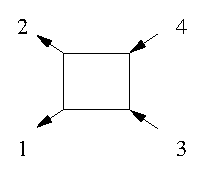
\epsfig{file=model/bare_vertex.eps}\\
Note that it may also be convenient to use the symmetric form
of the vertex function,
\begin{equation}
\Gamma^{(0)}_{\nu\sigma_1\nu\sigma_2,\nu\sigma_3\nu\sigma_4}(\mathbf{r}_1, \mathbf{r}_2; 
\mathbf{r}_3, \mathbf{r}_4)
 = \frac{U}{2}\, \delta_{\mathbf{r}_1,\mathbf{r}_2} 
\delta_{\mathbf{r}_3,\mathbf{r}_1} \delta_{\mathbf{r}_4,\mathbf{r}_2}
\left( \delta_{\sigma_1,\sigma_3}\delta_{\sigma_2,\sigma_4}
 - \vec{\sigma}_{\sigma_1,\sigma_3}\cdot
 \vec{\sigma}_{\sigma_2,\sigma_4} \right).
\end{equation}

Note that the vertex function is non-zero only in 
certain special cases:
\begin{eqnarray}
\sigma_1 = \sigma_3,\;\sigma_2 = \sigma_4 = -\sigma_1 & \to &
\Gamma^{(0)} = U \\
\sigma_1 = \sigma_4, \;\sigma_2 = \sigma_3 = -\sigma_1 & \to &
\Gamma^{(0)} = -U
\end{eqnarray}

In the Nambu representation we need to expand the vertex
to properly account for the mixed particle-hole basis
for the creation and annihilation operators.  If,
as before, we define
\begin{eqnarray}
\psi_{\mathbf{r}\nu 0} & = & c_{\mathbf{r}\nu\uparrow} \\   
\psi_{\mathbf{r}\nu 1} & = & c_{\mathbf{r}\nu\downarrow} \\
\psi_{\mathbf{r}\nu 2} & = & c^{\dagger}_{\mathbf{r}\nu\uparrow} \\
\psi_{\mathbf{r}\nu 3} & = & c^{\dagger}_{\mathbf{r}\nu\downarrow},
\end{eqnarray}
then we have additional terms in a vertex function
which is symmetrized within the particle-hole space.
All terms in the fully-symmetrized vertex can be represented
by the following vertex diagram for 
$\Gamma^{(0)}_{\nu\alpha_1\nu\alpha_2;\nu\alpha_3\nu\alpha_4}:$ \\
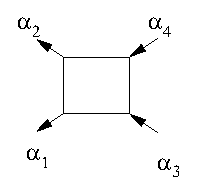
\epsfig{file=model/bare_vertex_mod.eps}\\

Here we show the relations for generalizing the vertex to
the expanded space.  Let $\overline{\alpha}$ represent
the operators that orginate from the expanded space, \textit{i.e.}
$\overline{c_{\uparrow}} = c^{\dagger}_{\uparrow}$.
\begin{eqnarray}
\Gamma^{(0)}_{\overline{1}2;\overline{3}4}
\psi^{\dagger}_{\overline{1}}\psi^{\dagger}_2
\psi_4 \psi_{\overline{3}}
& \equiv & 
\Gamma^{(0)}_{\overline{1}2;\overline{3}4}
\psi_1 \psi^{\dagger}_2
\psi_4 \psi^{\dagger}_3 \\
& = & -\Gamma^{(0)}_{\overline{1}2;\overline{3}4}
\psi^{\dagger}_2\psi_1 \psi_4 \psi^{\dagger}_3 \\
& = & -\Gamma^{(0)}_{\overline{1}2;\overline{3}4}
\psi^{\dagger}_2\psi^{\dagger}_3 \psi_1 \psi_4 \\
& \equiv & \Gamma^{(0)}_{23;41}\psi^{\dagger}_2\psi^{\dagger}_3 \psi_1 \psi_4 
\end{eqnarray}
From which we get
\begin{equation}
\Gamma^{(0)}_{\overline{1}2;\overline{3}4} = -\Gamma^{(0)}_{23;41}.
\end{equation}
\begin{eqnarray}
\Gamma^{(0)}_{1\overline{2};3\overline{4}}
\psi^{\dagger}_{1}\psi^{\dagger}_{\overline{2}}
\psi_{\overline{4}} \psi_3 \\
& = & \Gamma^{(0)}_{1\overline{2};3\overline{4}}
\psi^{\dagger}_{1}\psi_{2}
\psi^{\dagger}_{4} \psi_3 \\
& = & - \Gamma^{(0)}_{1\overline{2};3\overline{4}}
\psi^{\dagger}_{1}\psi^{\dagger}_{4}
\psi_{2} \psi_3 \\
& \equiv & \Gamma^{(0)}_{14;32}
\psi^{\dagger}_{1}\psi^{\dagger}_{4}
\psi_{2} \psi_3 \\
\end{eqnarray}
From which we get
\begin{equation}
\Gamma^{(0)}_{1\overline{2};3\overline{4}} = -\Gamma^{(0)}_{14;32}.
\end{equation}
\begin{eqnarray}
\Gamma^{(0)}_{1\overline{2};\overline{3}4}
\psi^{\dagger}_{1}\psi^{\dagger}_{\overline{2}}
\psi_4 \psi_{\overline{3}} \\
& \equiv & \Gamma^{(0)}_{1\overline{2};\overline{3}4}
\psi^{\dagger}_1\psi_2
\psi_4 \psi^{\dagger}_3 \\
& = & \Gamma^{(0)}_{1\overline{2};\overline{3}4}
\psi^{\dagger}_1\psi^{\dagger}_3
\psi_2 \psi_4 \\
& \equiv & \Gamma^{(0)}_{1 3; 4 2}
\psi^{\dagger}_1\psi^{\dagger}_3
\psi_2 \psi_4 
\end{eqnarray}
From which we get
\begin{equation}
\Gamma^{(0)}_{1\overline{2};\overline{3}4}
= \Gamma^{(0)}_{1 3; 4 2}
\end{equation}
\begin{eqnarray}
\Gamma^{(0)}_{\overline{1}2;3\overline{4}}
\psi^{\dagger}_{\overline{1}}\psi^{\dagger}_2
\psi_{\overline{4}} \psi_3 
&  \equiv &
\Gamma^{(0)}_{\overline{1}2;3\overline{4}}
\psi_1\psi^{\dagger}_2
\psi^{\dagger}_4 \psi_3  \\
& = & \Gamma^{(0)}_{\overline{1}2;3\overline{4}}
\psi^{\dagger}_2\psi^{\dagger}_4\psi_1\psi_3 \\
& \equiv & \Gamma^{(0)}_{24;31}
\psi^{\dagger}_2\psi^{\dagger}_4\psi_1\psi_3
\end{eqnarray}
from which we get
\begin{equation}
\Gamma^{(0)}_{\overline{1}2;3\overline{4}} =
\Gamma^{(0)}_{24;31}.
\end{equation}
Finally, we have
\begin{eqnarray}
\Gamma^{(0)}_{\overline{1}\overline{2};\overline{3}\overline{4}}
\psi^{\dagger}_{\overline{1}}\psi^{\dagger}_{\overline{2}}
\psi_{\overline{4}} \psi_{\overline{3}} 
&  \equiv &
\Gamma^{(0)}_{\overline{1}\overline{2};\overline{3}\overline{4}}
\psi_1\psi_2
\psi^{\dagger}_4 \psi^{\dagger}_3  \\
& = &
\Gamma^{(0)}_{\overline{1}\overline{2};\overline{3}\overline{4}}
\psi^{\dagger}_4 \psi^{\dagger}_3 \psi_1\psi_2 \\
& \equiv &
\Gamma^{(0)}_{4 3; 2 1} \psi^{\dagger}_4 \psi^{\dagger}_3 \psi_1\psi_2
\end{eqnarray}
from which we get
\begin{equation}
\Gamma^{(0)}_{\overline{1}\overline{2};\overline{3}\overline{4}} =
\Gamma^{(0)}_{4 3; 2 1}.
\end{equation}

For the single-band Hubbard model, the above produces
the following:
\begin{eqnarray}
\Gamma^{(0)}_{01;01} & = U  \;\;\;\; & \Gamma^{(0)}_{01;10} = -U \\
\Gamma^{(0)}_{03;03} & = -U \;\;\;\; & \Gamma^{(0)}_{03;30} = U \\
\Gamma^{(0)}_{02;13} & = U \;\;\;\; & \Gamma^{(0)}_{02;31} = -U \\
\\
\Gamma^{(0)}_{10;10} & = U \;\;\;\; & \Gamma^{(0)}_{10;01} = -U \\
\Gamma^{(0)}_{12;12} & = -U \;\;\;\; & \Gamma^{(0)}_{12;21} = U \\
\Gamma^{(0)}_{13;02} & = U \;\;\;\; & \Gamma^{(0)}_{13;20} = -U \\
\\
\Gamma^{(0)}_{23;23} & = U \;\;\;\; & \Gamma^{(0)}_{23;32} = -U \\
\Gamma^{(0)}_{21;21} & = -U \;\;\;\; & \Gamma^{(0)}_{21;12} = U \\
\Gamma^{(0)}_{20;31} & = U \;\;\;\; & \Gamma^{(0)}_{20;13} = -U \\
\\
\Gamma^{(0)}_{32;32} & = U \;\;\;\; & \Gamma^{(0)}_{32;23} = -U \\
\Gamma^{(0)}_{30;30} & = -U  \;\;\;\; & \Gamma^{(0)}_{30;03} = U \\
\Gamma^{(0)}_{31;20} & = U \;\;\;\; & \Gamma^{(0)}_{31;02} = -U 
\end{eqnarray}

It will be convenient in some cases to work with the bare vertex in 
the particle-hole channel.
Graphically, the particle-hole and standard
vertices are as follows:
\begin{center}
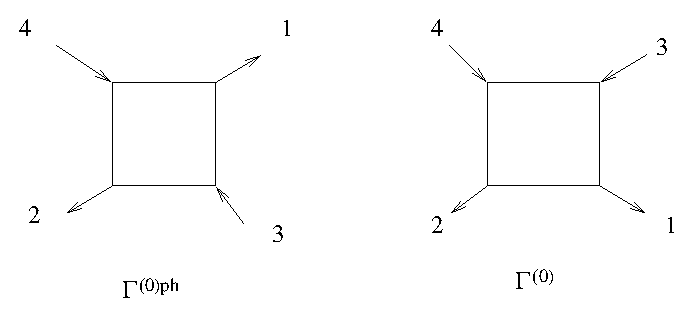
\epsfig{file=model/ph_vertex.eps}
\end{center}
For these to be equivalent representations of the vertex function
we must have
\begin{equation}
\Gamma^{(0)}_{1 2; 3 4}\psi_1^{\dagger}\psi_2^{\dagger};
\psi_4 \psi_3  = 
\Gamma^{(0)ph}_{1 3; 4 2} \psi_1^{\dagger}\psi_3
\psi_2^{\dagger}\psi_4.
\end{equation}
Since there are an even number of Fermi operator exchanges between
the left and right hand sides of the equation, we have
\begin{equation}
\Gamma^{(0)}_{1 2; 3 4} = \Gamma^{(0)ph}_{1 3; 4 2}.
\end{equation}

\chapter{Mixed analytical/numerical representation of the Green's function}
\label{chapter:grepresent}

Consider the following representation for the 
Green's function,
\begin{equation}
G(\varepsilon_n, \mathbf{r}) \equiv g(\varepsilon_n,\mathbf{r})
+ \tilde{G}(\varepsilon_n,\mathbf{r})
\end{equation}
where
\begin{equation}
\label{little_g}
\begin{split}
g(\varepsilon_n,\mathbf{r})  = & -( \Delta G(\mathbf{r})  - c_0(\mathbf{r}) )
Q_0(x_{00},\varepsilon_n) - c_0(\mathbf{r}) Q_0(x_{01}, \varepsilon_n) \\
& + (\Delta G^{\prime}(\mathbf{r}) - c_1(\mathbf{r}))
Q_1(x_{10},\varepsilon_n) + c_1(\mathbf{r})Q_1(x_{11},\varepsilon_n)
\end{split}
\end{equation}
In this case, $g$, $\Delta G$, $\Delta G^{\prime}$, $c_0$, and
$c_1$ are understood to be $2 \times 2$ matrices for each
value of $\mathbf{r}$.
Since $Q_0$ and $Q_1$ have special asymptotic properties
(as described in an appendix), the above functional
form for $g(\varepsilon_n,\mathbf{r})$ guarantees
that it contains the full $1/(i \varepsilon_n)$ and
$1/(i \varepsilon)^2$ contributions
to $G(\varepsilon_n, \mathbf{r})$
and $|\varepsilon_n| \to \infty$.

The $\mathbf{r}$-dependent 
numerical parameters $c_0(\mathbf{r})$ and $c_1(\mathbf{r})$ are used to
satisfy the following:
\begin{eqnarray}
\tilde{G}(\tau \to 0^+, \mathbf{r}) & = & 0 \\
\tilde{G}^{\prime}(\tau \to 0^+, \mathbf{r}) & = & 0.
\end{eqnarray}
These conditions do not
constrain the values 
for $x_{00}$, $x_{01}$, $x_{10}$, and $x_{11}$.
Thus, these parameters will be taken as fixed and independent
of $\mathbf{r}$.  Note that this is different from the
algorithm developed earlier.

To determine the values of $c_0$ and $c_1$ we
set $G(\tau \to 0^+, \mathbf{r}) = g(\tau \to 0^+, \mathbf{r})$
and $G^{\prime}(\tau \to 0^+, \mathbf{r}) = 
g^{\prime}(\tau \to 0^+, \mathbf{r})$.
The first condition gives
\begin{equation}
\begin{split}
G(\tau \to 0^+, \mathbf{r}) = &
- (\Delta G(\mathbf{r}) - c_0(\mathbf{r})) \,Q_0(x_{00},\tau \to 0^+)
 - c_0(\mathbf{r}) Q_0(x_{01}, \tau \to 0^+) \\
& +  (\Delta G^{\prime}(\mathbf{r}) - c_1(\mathbf{r})) \,Q_1(x_{10},\tau \to 0^+)
+ c_1(\mathbf{r}) \,Q_1(x_{11},\tau \to 0^+).
\end{split}
\end{equation}
Since
\begin{eqnarray}
Q_0(x_{0\alpha},\tau \to 0^+) & = & -\,\frac{1}{2} \\
Q_1(x_{1\alpha},\tau \to 0^+) & = & -\,\frac{1}{2 x_{1\alpha}}
\tanh(\beta x_{1\alpha}/2)
\end{eqnarray}
we get
\begin{equation}
\begin{split}
G(\tau \to 0^+, \mathbf{r}) = &
          - (\Delta G(\mathbf{r}) - c_0(\mathbf{r}))(-\frac{1}{2}) -
       c_0(\mathbf{r})(-\frac{1}{2}) \\
& + (\Delta G^{\prime}(\mathbf{r}) - c_1(\mathbf{r}))
\frac{- \tanh(\beta x_{10} / 2)}{2 x_{10}}
+ c_1(\mathbf{r}) \frac{- \tanh(\beta x_{11} / 2)}{2 x_{11}}
\end{split}
\end{equation}
After simplification we get
\begin{equation}
\begin{split}
G(\tau \to 0^+, \mathbf{r}) = &
\frac{\Delta G(\mathbf{r})}{2}  - \frac{\Delta G^{\prime}(\mathbf{r})
\,\tanh(\beta x_{10}/2)}{2 x_{10}} \\
& + c_1(\mathbf{r}) \left[ \frac{\tanh(\beta x_{10}/2)}{2 x_{10}}
 - \frac{\tanh(\beta x_{11}/2)}{2 x_{11}} \right]
\end{split}
\end{equation}
after which it is simple to solve for $c_1(\mathbf{r})$.   We get
\begin{equation}
c_1(\mathbf{r}) = \frac{G(\tau \to 0^+, \mathbf{r}) - 
\frac{\Delta G(\mathbf{r})}{2}
+ \frac{\Delta G^{\prime}(\mathbf{r})
\,\tanh(\beta x_{10}/2)}{2 x_{10}}}{
\left[\frac{\tanh(\beta x_{10}/2)}{2 x_{10}}
 - \frac{\tanh(\beta x_{11}/2)}{2 x_{11}} \right]}.
\end{equation} 

The second condition gives us
\begin{equation}
\label{g_prime}
\begin{split}
G^{\prime}(\tau \to 0^+, \mathbf{r}) = &
- (\Delta G(\mathbf{r}) - c_0(\mathbf{r})) 
\,Q_0^{\prime}(x_{00},\tau \to 0^+)
 - c_0(\mathbf{r}) Q_0^{\prime}(x_{01}, \tau \to 0^+) \\
& +  (\Delta G^{\prime}(\mathbf{r}) - c_1(\mathbf{r})) 
\,Q_1^{\prime}(x_{10},\tau \to 0^+)
+ c_1(\mathbf{r}) \,Q_1^{\prime}(x_{11},\tau \to 0^+).
\end{split}
\end{equation}
Since
\begin{eqnarray}
Q_0^{\prime}(x_{0\alpha},\tau \to 0^+) & = & \frac{x_{0\alpha}}{2}
\tanh(\beta x_{0\alpha}/2) \\
Q_1^{\prime}(x_{1\alpha},\tau \to 0^+) & = & \frac{1}{2}
\end{eqnarray}
Eq.~(\ref{g_prime}) becomes
\begin{equation}
\begin{split}
G^{\prime}(\tau \to 0^+, \mathbf{r}) = &
- (\Delta G(\mathbf{r}) - c_0(\mathbf{r})) \frac{x_{00}}{2} 
\tanh(\beta x_{00}/2) - c_0(\mathbf{r}) \frac{x_{01}}{2} 
\tanh(\beta x_{01}/2) \\
& +  (\Delta G^{\prime}(\mathbf{r}) - c_1(\mathbf{r}))\frac{1}{2}
+ c_1(\mathbf{r})\frac{1}{2}.
\end{split}
\end{equation}
After simplification we get
\begin{equation}
\begin{split}
G^{\prime}(\tau \to 0^+, \mathbf{r}) = &
\frac{1}{2}\Delta G^{\prime}(\mathbf{r}) -
 \Delta G(\mathbf{r}) \frac{x_{00}}{2} 
\tanh(\beta x_{00}/2) \\
& + c_0(\mathbf{r}) \left(\frac{x_{00}}{2} \tanh(\beta x_{00}/2)
- \frac{x_{01}}{2} \tanh(\beta x_{01}/2) \right).
\end{split}
\end{equation}
Finally, we solve for $c_0(\mathbf{r})$ to get
\begin{equation}
c_0(\mathbf{r}) = \frac{ G^{\prime}(\tau \to 0^+, \mathbf{r}) -
\frac{1}{2}\Delta G^{\prime}(\mathbf{r}) +
 \Delta G(\mathbf{r}) \frac{x_{00}}{2} 
\tanh(\beta x_{00}/2) }
{\left(\frac{x_{00}}{2} \tanh(\beta x_{00}/2)
- \frac{x_{01}}{2} \tanh(\beta x_{01}/2) \right)}.
\end{equation}

It is convenient to rewrite Eq.~(\ref{little_g})
in the following mathematically equivalent form:
\begin{equation}
g(\tau, \mathbf{r}) = \sum_{\alpha = 0,1; \beta = 0, 1}
c_{\alpha\beta}(\mathbf{r}) Q_{\alpha\beta}(\tau).
\end{equation}
Here we set
\begin{eqnarray}
Q_{00}(\tau) & \equiv & Q_0(x_{00},\tau) \\
Q_{01}(\tau) & \equiv & Q_0(x_{00},\tau) \\
Q_{10}(\tau) & \equiv & Q_1(x_{10},\tau) \\
Q_{11}(\tau) & \equiv & Q_1(x_{11},\tau). 
\end{eqnarray}
In this modified representation we have
\begin{eqnarray}
c_{01}(\mathbf{r}) & = & - \frac{ G^{\prime}(\tau \to 0^+, \mathbf{r}) -
\frac{1}{2}\Delta G^{\prime}(\mathbf{r}) +
 \Delta G(\mathbf{r}) \frac{x_{00}}{2} 
\tanh(\beta x_{00}/2) }
{\left(\frac{x_{00}}{2} \tanh(\beta x_{00}/2)
- \frac{x_{01}}{2} \tanh(\beta x_{01}/2) \right)} \\
c_{00}(\mathbf{r}) & = & - \Delta G(\mathbf{r}) - 
c_{01}(\mathbf{r}) \\
c_{11}(\mathbf{r}) & = & \frac{G(\tau \to 0^+, \mathbf{r}) - 
\frac{\Delta G(\mathbf{r})}{2}
+ \frac{\Delta G^{\prime}(\mathbf{r})
\,\tanh(\beta x_{10}/2)}{2 x_{10}}}{
\left[\frac{\tanh(\beta x_{10}/2)}{2 x_{10}}
 - \frac{\tanh(\beta x_{11}/2)}{2 x_{11}} \right]} \\
c_{10}(\mathbf{r}) & = & \Delta G^{\prime}(\mathbf{r}) - c_{11}(\mathbf{r}).
\end{eqnarray}

On the first iteration (where the values of $G(\tau \to 0^{+},\mathbf{r})$
and $G^{\prime}(\tau \to 0^+,\mathbf{r})$ are unknown), we set
$c_{01}(\mathbf{r}) = 0$, $c_{00}(\mathbf{r}) = - \Delta G(\mathbf{r})$,
$c_{11}(\mathbf{r}) = 0$, and $c_{10}(\mathbf{r}) =
\Delta G^{\prime}(\mathbf{r})$.
This choice guarantees, at least, that $g(\tau,\mathbf{r})$ will
have the correct asymptotic properties.



\chapter{First-order self-energy and single-particle expectation values}
\label{first-order}

\section{Self-energy}
\label{first-order-self-energy}
The first-order diagram is
represented graphically as 
\begin{center}
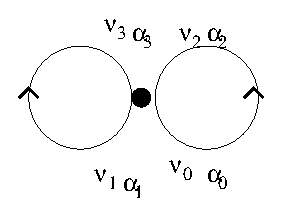
\epsfig{file=flex/phi_first.eps} 
\end{center}
and mathematically as
\begin{equation}
\Phi^{(1)} = \frac{T}{4} \sum_{\mathbf{r}_1} \int_0^{\beta}d\tau_1
\sum_{\nu_0\alpha_0\nu_1 \alpha_1\nu_2\alpha_2 \nu_3 \alpha_3} 
\Gamma^{(0)}_{\nu_0\alpha_0\nu_1\alpha_1; \nu_2\alpha_2 \nu_3\alpha_3}
G_{\nu_3\alpha_3\nu_1\alpha_1}(\tau_1,\mathbf{r}_1;\tau_1,\mathbf{r}_1)
\,G_{\nu_2\alpha_2\nu_0\alpha_0}(\tau_1,\mathbf{r}_1;\tau_1,\mathbf{r}_1) 
\end{equation}

The first order self-energy is obtained with
\begin{equation}
\Sigma^{(1)}_{\nu\alpha \nu^{\prime}\alpha^{\prime}}(x,x^{\prime})  =
T \frac{\delta\; \Phi^{(1)}}
{\delta\; G_{\nu^{\prime}\alpha^{\prime}\nu \alpha}(x^{\prime},x)} 
\end{equation}
which in this case yields
\begin{equation}
\begin{split}
\Sigma^{(1)}_{\nu\alpha \nu^{\prime}\alpha^{\prime}}(x,x^{\prime})
= & \frac{T^2}{2} \sum_{\nu_0\alpha_0 \nu_2\alpha_2;\nu_1 \alpha_1 \nu_3\alpha_3}
\int_{0}^{\beta}d\tau_1 \sum_{\mathbf{r}_1}
\Gamma^{(0)}_{\nu_0\alpha_0 \nu_1\alpha_1; \nu_2\alpha_2 \nu_3 \alpha_3}
G_{\nu_2\alpha_2\nu_0 \alpha_0}(\tau_1,\mathbf{r}_1;\tau_1,\mathbf{r}_1)
\delta_{\nu^{\prime}\alpha^{\prime},\nu_3\alpha_3}\,\delta_{\nu\alpha,\nu_1\alpha_1}
\delta_{\mathbf{r},\mathbf{r}_1} \delta_{\mathbf{r}^{\prime},\mathbf{r}_1} 
\\
& \times\,
\frac{\delta(\tau - \tau_1)}{T}\,\frac{\delta(\tau^{\prime} - \tau_1)}{T}
\end{split}
\end{equation}
which becomes
\begin{equation}
\Sigma^{(1)}_{\nu\alpha \nu^{\prime}\alpha^{\prime}}(x,x^{\prime}) =
\frac{1}{2}\sum_{\nu_0\alpha_0 \nu_2\alpha_2}
\Gamma^{(0)}_{\nu_0\alpha_0\nu\alpha; \nu_2\alpha_2 \nu^{\prime}\alpha^{\prime}}
G_{\nu_2\alpha_2 \nu_0\alpha_0}(\tau,\mathbf{r};\tau,\mathbf{r})\,
\delta_{\mathbf{r},\mathbf{r}^{\prime}} \, \delta(\tau - \tau^{\prime})
\end{equation}
Graphically, this self energy is represented as\\
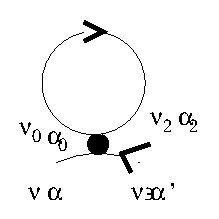
\epsfig{file=flex/sigma_first.eps}\\
The overall positive sign comes from having a (-1) from one
occurence of the interaction and another (-1) for having
a closed loop.

For a translationally invariant system we have (after changing
the internal subscript ``2'' to ``1'')
\begin{equation}
\Sigma^{(1)}_{\nu\alpha \nu^{\prime}\alpha^{\prime}}(\tau,\mathbf{r}) =
\frac{1}{2} \sum_{\nu_0\alpha_0 \nu_1\alpha_1}
\Gamma^{(0)}_{\nu_0\alpha_0\alpha;\nu_1 \alpha_1 \nu^{\prime}\alpha^{\prime}}
G_{\nu_1\alpha_1 \nu_0\alpha_0}(\tau=0,\mathbf{r}=\mathbf{0})\,
\delta_{\mathbf{r},\mathbf{0}} \, \delta(\tau)
\end{equation}
There is an ambiguity as to whether take $\tau \to 0^+$ or
$\tau \to 0^-$.  If $\alpha_1 \neq \alpha_0$ and/or $\nu_1 \neq \nu_0$, 
then this
ambiguity is irrelevant.  However, if $\alpha_1 = \alpha_0$
and $\nu_1 = \nu_0$,
then the $\tau \to 0^-$ limit should be used if $\alpha_0$
and $\alpha_1$ correspond to particle degrees of freedom (0,1)
and $\tau \to 0^+$ should be used for hole degrees of freedom
(2,3).

Since the self-energy is local in time and space, its Fourier
transform is independent of frequency and momentum.  We have
\begin{equation}
\Sigma^{(1)}_{\nu\alpha \nu^{\prime}\alpha^{\prime}}(\epsilon_n,\mathbf{k}) \equiv
\Sigma^{(1)}_{\nu\alpha \nu^{\prime}\alpha^{\prime}} =
\frac{1}{2} \sum_{\nu_0\alpha_0 \nu_1\alpha_1}
\Gamma^{(0)}_{\nu_0\alpha_0\nu\alpha; \nu_1\alpha_1 \nu^{\prime}\alpha^{\prime}}
G_{\nu_1\alpha_1 \nu_0\alpha_0}(\tau=0,\mathbf{r}=\mathbf{0})
\end{equation}

For concretness, consider the single band case to see how the above formula
is able to reproduce well know results.
Using the definition of $\Gamma^{(0)}$ from Chapter~\ref{chapter:bare_vertex},
we obtain the following explicit forms for the $\Sigma^{(1)}$
where the spatial part of the Green's function is assumed to
be evaluated at $\mathbf{r} = \mathbf{0}$:
\begin{eqnarray}
\Sigma^{(1)}_{00} & = &
\frac{1}{2}\sum_{\alpha_0\beta_0} \Gamma^{(0)}_{\alpha_0 0; \beta_0 0}
G_{\beta_0 \alpha_0}(\tau =0, \mathbf{r}=\mathbf{0}) \\
    & = & \frac{1}{2}\left(U G_{11}(\tau = 0^-) - 
        U G_{33}(\tau = 0^+) \right)\\
    & = & U\, G_{11}(\tau = 0^-) 
\end{eqnarray}
\begin{eqnarray}
\Sigma^{(1)}_{01} & = &
\frac{1}{2}\sum_{\alpha_0\beta_0} \Gamma^{(0)}_{\alpha_0 0; \beta_0 1}
G_{\beta_0 \alpha_0}(\tau =0, \mathbf{r}=\mathbf{0}) \\
    & = & \frac{1}{2}\left(-U G_{01}(\tau = 0) + 
U G_{32}(\tau = 0)\right) \\
    & = & -U\, G_{01}(\tau = 0)
\end{eqnarray}
\begin{eqnarray}
\Sigma^{(1)}_{02} & = &
\frac{1}{2}\sum_{\alpha_0\beta_0} \Gamma^{(0)}_{\alpha_0 0; \beta_0 2}
G_{\beta_0 \alpha_0}(\tau =0, \mathbf{r}=\mathbf{0}) \\
    & = & 0  \;\;\textrm{(no non-zero vertices)}
\end{eqnarray}
\begin{eqnarray}
\Sigma^{(1)}_{03} & = &
\frac{1}{2}\sum_{\alpha_0\beta_0} \Gamma^{(0)}_{\alpha_0 0; \beta_0 3}
G_{\beta_0 \alpha_0}(\tau =0, \mathbf{r}=\mathbf{0}) \\
    & = & \frac{1}{2}\left(-U G_{12}(\tau = 0) + U G_{03}(\tau = 0)\right) \\
    & = & U\, G_{03}(\tau = 0) 
\end{eqnarray}
\begin{eqnarray}
\Sigma^{(1)}_{10} & = &
\frac{1}{2}\sum_{\alpha_0\beta_0} \Gamma^{(0)}_{\alpha_0 1; \beta_0 0}
G_{\beta_0 \alpha_0}(\tau =0, \mathbf{r}=\mathbf{0}) \\
    & = & \frac{1}{2}\left(-U G_{10}(\tau = 0) + 
U G_{23}(\tau = 0)\right) \\
    & = & -U\, G_{10}(\tau = 0)
\end{eqnarray}
\begin{eqnarray}
\Sigma^{(1)}_{11} & = &
\frac{1}{2}\sum_{\alpha_0\beta_0} \Gamma^{(0)}_{\alpha_0 1; \beta_0 1}
G_{\beta_0 \alpha_0}(\tau =0, \mathbf{r}=\mathbf{0}) \\
    & = & \frac{1}{2}\left(U G_{00}(\tau = 0^-)  
- U G_{22}(\tau = 0^+)\right) \\
    & = & U\, G_{00}(\tau = 0^-)
\end{eqnarray}
\begin{eqnarray}
\Sigma^{(1)}_{12} & = &
\frac{1}{2}\sum_{\alpha_0\beta_0} \Gamma^{(0)}_{\alpha_0 1; \beta_0 2}
G_{\beta_0 \alpha_0}(\tau =0, \mathbf{r}=\mathbf{0}) \\
    & = & \frac{1}{2}\left(U G_{12}(\tau = 0) 
- U G_{03}(\tau = 0)\right) \\
    & = & -U\, G_{03}(\tau = 0)
\end{eqnarray}
\begin{eqnarray}
\Sigma^{(1)}_{22} & = &
\frac{1}{2}\sum_{\alpha_0\beta_0} \Gamma^{(0)}_{\alpha_0 2; \beta_0 2}
G_{\beta_0 \alpha_0}(\tau =0, \mathbf{r}=\mathbf{0}) \\
    & = & \frac{1}{2}\left(-U G_{11}(\tau = 0^-) + 
U G_{33}(\tau = 0^+)\right) \\
    & = & -U\, G_{11}(\tau = 0^-) = -\Sigma^{(1)}_{00} 
\end{eqnarray}
In matrix form $\Sigma^{(1)}$ is given by
\begin{equation}
\Sigma^{(1)} = 
U 
\begin{pmatrix}
G_{11} & -G_{01} & 0 & G_{03} \\
-G_{10} & G_{00} & -G_{03} & 0 \\
0  & -G_{30} & -G_{11} & G_{10} \\
G_{30} & 0 & G_{01} & -G_{00}
\end{pmatrix}
\end{equation}

\section{$\mathrm{Tr}\; \Sigma^{(1)} G$}

This trace is needed in the evaluation of the thermodynamic
potential.  For this trace we have
\begin{eqnarray}
\mathrm{Tr}\; \Sigma^{(1)} G & \equiv &
      T \sum_{\mathbf{k},\varepsilon_n}
 \textrm{Tr}\, \Sigma^{(1)}\, 
G(\varepsilon_n,\mathbf{k})
\\
& = & 
  N_{sites} 
\mathrm{Tr}\; \Sigma^{(1)} G(\tau=0,\mathbf{r}=\mathbf{0}) \\
 & = &   N_{sites} 
\mathrm{Tr}\; U
\begin{pmatrix}
G_{11} & -G_{01} & 0 & G_{03} \\
-G_{10} & G_{00} & -G_{03} & 0 \\
0  & -G_{30} & -G_{11} & G_{10} \\
G_{30} & 0 & G_{01} & -G_{00}
\end{pmatrix}
\begin{pmatrix}
G_{00} & G_{01} & G_{02} & G_{03} \\
G_{10} & G_{11} & G_{12} & G_{13} \\
G_{20}  & G_{21} & G_{22} & G_{23} \\
G_{30} & G_{31} & G_{32} & G_{33}
\end{pmatrix}
\\
& = &
 N_{sites} 
\mathrm{Tr}\; U
\begin{pmatrix}
G_{11} & -G_{01} & 0 & G_{03} \\
-G_{10} & G_{00} & -G_{03} & 0 \\
0  & -G_{30} & -G_{11} & G_{10} \\
G_{30} & 0 & G_{01} & -G_{00}
\end{pmatrix}
\begin{pmatrix}
G_{00} & G_{01} & G_{02} & G_{03} \\
G_{10} & G_{11} & -G_{03} & G_{13} \\
G_{20}  & -G_{30} & -G_{00} & G_{23} \\
G_{30} & G_{31} & G_{32} & -G_{11}
\end{pmatrix}
\\
& = & 4 N_{sites} U (G_{11}G_{00} - G_{01}G_{10} + G_{03}G_{30}) 
\end{eqnarray}
In the above we have used the symmetries of the Green's function
described in Chapter~\ref{chapter:g0}.

The last term in the above gives the BCS-like contribution to
the condensation energy for an $s$-wave superconductor.  The 
first term is the normal Hartree energy, $<n_{\uparrow}><n_{\downarrow}>$.
The nature of the middle term is more clear when we note that
\begin{eqnarray}
G_{00} & = & \frac{1}{2}( n + m_z) \\
G_{11} & = & \frac{1}{2}( n - m_z) \\
G_{01} & = & \frac{1}{2}( m_x + i m_y) \\
G_{10} & = & \frac{1}{2}( m_x - i m_y)
\end{eqnarray}
Upon substitution we find that
\begin{equation}
\mathrm{Tr}\; \Sigma^{(1)} G = 4 N_{sites} U 
\left( \frac{1}{4} n^2 - \frac{1}{4}(m_x^2 + m_y^2 + m_z^2)
+ G_{03}G_{30} \right)
\end{equation}
Thus, the $G_{01}G_{10}$ term is needed to account for
polarization in the $x$ or $y$ directions.

\section{Evaluation of average single-particle energies}

The average value of the kinetic energy is easiest
to evaluate in $\mathbf{k}$-space.  We have
\begin{eqnarray}
\frac{<KE>}{N_L} & = & \frac{1}{N_L}
\sum_{\mathbf{k}\nu\nu^{\prime}\sigma} \epsilon_{\nu\nu^{\prime}}(\mathbf{k}) 
<c^{\dagger}_{\mathbf{k}\nu\sigma} c_{\mathbf{k}\nu^{\prime}\sigma}>
\\
& = & \frac{1}{N_L} \sum_{\mathbf{k}\nu\nu^{\prime}\sigma} 
\epsilon_{\nu\nu^{\prime}}(\mathbf{k}) 
G_{\nu^{\prime}\sigma \nu\sigma}(\tau \to 0^-, \mathbf{k}) 
\end{eqnarray}

The magnetic field coupling energy is simplest to evaluate
in real-space.  There it is given by
\begin{eqnarray}
\frac{<E_{mag}>}{N_L} & = & - \frac{1}{N_L} 
\sum_{\mathbf{r}\nu\sigma\sigma^{\prime}} \mathbf{h}\cdot 
\vec{\sigma}_{\sigma\sigma^{\prime}}
 <c^{\dagger}_{\mathbf{r}\nu\sigma} c_{\mathbf{r}\nu\sigma^{\prime}}>
 \\
& = & - \sum_{\nu\sigma\sigma^{\prime}} 
\mathbf{h}\cdot\vec{\sigma}_{\sigma\sigma^{\prime}}\,
G_{\nu\sigma^{\prime}\nu\sigma}(\tau \to 0^-,\mathbf{r} = \mathbf{0}) 
\end{eqnarray}.

\section{Updating $\phi(\mathbf{r})$}

Recall that
\begin{equation}
H_{p}  = -\frac{h_p}{2} 
\left( \sum_{\mathbf{r}\mathbf{r}^{\prime}
\nu\nu^{\prime}\sigma\sigma^{\prime}}  
\Psi_{\nu\sigma\nu^{\prime}\sigma^{\prime}}(\mathbf{r},\mathbf{r}^{\prime})
 c_{\mathbf{r}\nu\sigma}c_{\mathbf{r}^{\prime}\nu^{\prime}\sigma^{\prime}} + 
\Psi_{\nu^{\prime}\sigma^{\prime}\nu\sigma}^*(\mathbf{r}^{\prime},\mathbf{r})
c^{\dagger}_{\mathbf{r}\nu\sigma}
 c^{\dagger}_{\mathbf{r}^{\prime}\nu^{\prime}\sigma^{\prime}}\right)
\end{equation}
so that
\begin{equation}
E_p \equiv <H_p> 
= -\frac{h_p}{2} 
\left( \sum_{\mathbf{r}\mathbf{r}^{\prime}\nu\nu^{\prime}\sigma\sigma^{\prime}}  
\Psi_{\nu\sigma\nu^{\prime}\sigma^{\prime}}(\mathbf{r},\mathbf{r}^{\prime})
<c_{\mathbf{r}\nu\sigma}c_{\mathbf{r}^{\prime}\nu^{\prime}\sigma^{\prime}}> + 
\Psi_{\nu^{\prime}\sigma^{\prime}\nu\sigma}^*(\mathbf{r}^{\prime},\mathbf{r})
 <c^{\dagger}_{\mathbf{r}\nu\sigma}
 c^{\dagger}_{\mathbf{r}^{\prime}\nu^{\prime}\sigma^{\prime}}>\right)
\end{equation}
The expectation values represents the
equal-time, spatially-dependent
induced pairing magnitude.
We define the \textit{induced} pairing state, $\Psi^{\prime}$
and \textit{induced} pairing amplitude, $m_p $, by
\begin{equation}
<c_{\mathbf{r}\nu\sigma}c_{\mathbf{r}^{\prime}\nu^{\prime}\sigma^{\prime}}>  =  m_p 
\left(\Psi^{\prime}_{\nu^{\prime}\sigma^{\prime}\mu\sigma}(\mathbf{r}^{\prime},
\mathbf{r})\right)^* 
\end{equation}
which implies that
\begin{equation}
<c^{\dagger}_{\mathbf{r}\nu\sigma} 
c^{\dagger}_{\mathbf{r}^{\prime}\nu^{\prime}\sigma^{\prime}}>  = 
m_p \Psi^{\prime}_{\nu\sigma\nu^{\prime}\sigma^{\prime}}(\mathbf{r},\mathbf{r}^{\prime}).
\end{equation}
\begin{eqnarray}
E_p & =  & - \frac{h_p m_p}{2} 
\sum_{\mathbf{r}\mathbf{r}^{\prime}\nu\nu^{\prime}\sigma\sigma^{\prime}} 
\Psi_{\nu\sigma\nu^{\prime}\sigma^{\prime}}(\mathbf{r},\mathbf{r}^{\prime}) 
\left(\Psi^{\prime}_{\nu^{\prime}\sigma^{\prime}\nu\sigma}
(\mathbf{r}^{\prime},\mathbf{r})\right)^* +
\left(\Psi_{\nu^{\prime}\sigma^{\prime}\nu\sigma}(\mathbf{r}^{\prime},
\mathbf{r})\right)^* 
\Psi^{\prime}_{\nu\sigma\nu^{\prime}\sigma^{\prime}}(\mathbf{r},\mathbf{r}^{\prime})
\\
& = &
- h_p m_p \;\textrm{Re }
\left(\sum_{\mathbf{r}\mathbf{r}^{\prime}\nu\nu^{\prime}\sigma\sigma^{\prime}} 
\Psi_{\nu\sigma\nu\sigma^{\prime}}(\mathbf{r},\mathbf{r}^{\prime}) 
\left(\Psi^{\prime}_{\nu^{\prime}\sigma^{\prime}\nu\sigma}
(\mathbf{r}^{\prime},\mathbf{r})\right)^* \right)  
\end{eqnarray} 
For a translationally invariant system this reduces to
\begin{equation}
\frac{<E_p>}{N_L}  =  - 
h_p m_p\;\textrm{Re } \sum_{\mathbf{r}\nu\nu^{\prime}\sigma\sigma^{\prime}}
    \phi_{\nu\sigma\nu^{\prime}\sigma^{\prime}}(\mathbf{r}) 
\left(\phi^{\prime}_{\nu^{\prime}\sigma^{\prime}\nu\sigma}(-\mathbf{r})\right)^* 
\end{equation}

To find the strongest pairing channel, we want the applied
pair field to couple directly to the induced pairing wave function,
\textit{i.e.} $\phi = \phi^{\prime}$.  Thus, on each iteration
we determine $\phi^{\prime}$ from
\begin{equation}
<c^{\dagger}_{\mathbf{r}^{\prime}\nu^{\prime}\sigma^{\prime}} 
c^{\dagger}_{\mathbf{r}\nu\sigma}> = 
m_p \Psi^{\prime}_{\nu\sigma\nu^{\prime}\sigma^{\prime}}(\mathbf{r},\mathbf{r}^{\prime})
\end{equation}
so that in the translationally invariant case (and assuming
$n_p = 0$)
\begin{equation} 
<c^{\dagger}_{\mathbf{r}^{\prime}\nu^{\prime}\sigma^{\prime}} 
c^{\dagger}_{\mathbf{r}\nu\sigma}>  =  m_p 
\,\phi_{\nu\sigma\nu^{\prime}\sigma^{\prime}}^{\prime}(\mathbf{r} -
\mathbf{r}^{\prime}) 
\end{equation}
The left hand side is obtained from the equal time Green's
function.  Namely
\begin{eqnarray} 
<c^{\dagger}_{\mathbf{r}^{\prime}\nu^{\prime}\sigma^{\prime}} 
c^{\dagger}_{\mathbf{r}\nu\sigma}> & \equiv &
<\psi^{\dagger}_{\mathbf{r}^{\prime}\nu^{\prime}\sigma^{\prime}}
\psi_{\mathbf{r}\nu\overline{\sigma}}> \\
& = & 
G_{\nu\overline{\sigma}\nu^{\prime}\sigma^{\prime}}(\mathbf{r}-\mathbf{r}^{\prime},
\tau \to 0-).
\end{eqnarray}

Thus, $\phi_{\nu\sigma\nu^{\prime}\sigma^{\prime}}(\mathbf{r})$ 
is obtained by normalizing  
$G_{\nu\overline{\sigma}\nu^{\prime}\sigma^{\prime}}(\tau \to 0^-, \mathbf{r})$.
The normalization constant is the pairing strength, $m_p$.
Finally, to iterate our pairing field 
to the strongest pairing channel, we set
$\phi = \phi^{\prime}$ on each iteration
as new results for $G(\tau \to 0^-, \mathbf{r})$
are computed.  

\chapter{Particle-hole diagrams}
\label{chapter:particle-hole}

\section{Self-energy}
The particle-hole free-energy diagrams are given by
the following series:

\begin{center}
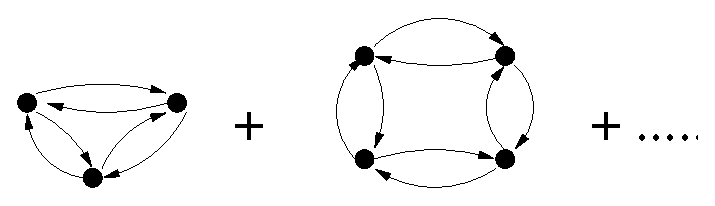
\epsfig{file=flex/phi_ph.eps}
\end{center}

Let $\chi^{ph}_{\nu_3\alpha_3 \nu_2 \alpha_2; 
\nu_1\alpha_1 \nu_0\alpha_0}(x_1,x_0)$ refer
to the following diagram:

\begin{center}
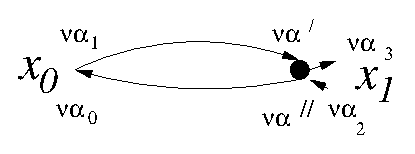
\epsfig{file=flex/chi_ph.eps}
\end{center}

Here $x$ refers to the space time label, $(\mathbf{r},\tau)$.
Mathematically, the above diagram is represented as
\begin{eqnarray}
\label{k_ph}
\chi^{ph}_{\nu_3\alpha_3 \nu_2 \alpha_2; \nu_1 \alpha_1 \nu_0\alpha_0}(x_1,x_0) 
& = & \frac{1}{2} \sum_{\nu^{\prime}\alpha^{\prime}\nu^{\prime\prime} \alpha^{\prime\prime}}
\Gamma^{(0)ph}_{\nu_3\alpha_3\nu_2\alpha_2; 
\nu^{\prime}\alpha^{\prime}\nu^{\prime\prime}\alpha^{\prime\prime}}\,
G_{\nu^{\prime}\alpha^{\prime}\nu_1 \alpha_1}(x_1,x_0) \; G_{\nu_0\alpha_0 
\nu^{\prime\prime}\alpha^{\prime\prime}}(x_0,x_1) \\
& = & -\frac{1}{2}\sum_{\nu^{\prime}\alpha^{\prime}\nu^{\prime\prime} \alpha^{\prime\prime}} 
\Gamma^{(0)ph}_{\nu_3\alpha_3 \nu_2 \alpha_2; \nu^{\prime}\alpha^{\prime}
\nu^{\prime\prime}\alpha^{\prime\prime}}\,
\tilde{\chi}^{ph}_{\nu^{\prime}\alpha^{\prime}\nu^{\prime\prime} \alpha^{\prime\prime}; 
\nu_1\alpha_1\nu_0\alpha_0 \beta_0}(x_1,x_0)
\end{eqnarray}
where
\begin{equation}
\label{chi_ph}
\tilde{\chi}^{ph}_{\nu^{\prime}\alpha^{\prime}\nu^{\prime\prime}\alpha^{\prime\prime}; 
\nu_1\alpha_1 \nu_0\alpha_0}(x_1,x_0) \equiv
(-1) G_{\nu^{\prime}\alpha^{\prime}\nu_1 \alpha_1}(x_1,x_0) \; 
G_{\nu_0\alpha_0 \nu^{\prime\prime}\alpha^{\prime\prime}}(x_0,x_1).
\end{equation}

For a translationally invariant system we have
\begin{equation}
\tilde{\chi}^{ph}_{\nu^{\prime}\alpha^{\prime}\nu^{\prime\prime}\alpha^{\prime\prime}; 
\nu_1\alpha_1 \nu_0\alpha_0}(\tau,\mathbf{r}) \equiv
(-1) G_{\nu^{\prime}\alpha^{\prime}\nu_1 \alpha_1}(\tau,\mathbf{r}) \; 
G_{\nu_0\alpha_0 \nu^{\prime\prime}\alpha^{\prime\prime}}(-\tau,\mathbf{r})
\end{equation}
It is convenient to combine $\nu^{\prime}\alpha^{\prime}\nu^{\prime\prime}
\alpha^{\prime\prime}$
into a single index, $\gamma^{\prime} \equiv
4 n_b(4\nu^{\prime}+ \alpha^{\prime}) + (4\nu^{\prime\prime} + 
\alpha^{\prime\prime})$ with the same
for a single index $\gamma_0$ in
terms of $\nu_1\alpha_1\nu_0\alpha_0$.  We then have
\begin{equation}
\tilde{\chi}^{ph}_{\gamma^{\prime},\gamma_0}(\tau,\mathbf{r}) \equiv
\tilde{\chi}^{ph}_{\nu^{\prime}\alpha^{\prime}\nu^{\prime\prime}\alpha^{\prime\prime}; 
\nu_1\alpha_1 \nu_0\alpha_0}(\tau,\mathbf{r})
\end{equation}
The same can be done for $\Gamma^{(0)ph}$ such that
\begin{equation}
\chi^{ph}_{\nu_3\alpha_3\nu_2\alpha_2;\nu_1\alpha_1\nu_0\alpha_0}(\tau,\mathbf{r}) 
=-\frac{1}{2} \sum_{\alpha^{\prime}\beta^{\prime}} 
\Gamma^{(0)ph}_{\nu_3\alpha_3\nu_2\alpha_2;\nu^{\prime}\alpha^{\prime}
\nu^{\prime\prime}\alpha^{\prime\prime}}
\tilde{\chi}^{ph}_{\nu^{\prime}\alpha^{\prime}\nu^{\prime\prime}\alpha^{\prime\prime};
\nu_1\alpha_1\nu_0\alpha_0}
(\tau,\mathbf{r})
\end{equation}
can be interpretted as a simple matrix equation for each combination
of $\tau$ and $\mathbf{r}$ values:
\begin{equation}
\left[\chi^{ph}(\tau,\mathbf{r})\right]_{\gamma_1,\gamma_0} =
-\frac{1}{2}
\left[\Gamma^{(0)}\,\tilde{\chi}^{ph}(\tau,\mathbf{r})\right]_{\gamma_1,\gamma_0}
\end{equation}
where $\chi^{ph}$, $\Gamma^{(0)ph}$, and $\tilde{\chi}^{ph}$
are taken as $16n_b^2 \times 16n_b^2$ matrices using the indexing scheme
described above.

This simplifies the representation of $\Phi_{ph}$.  For
example, we can write
\begin{equation}
\nonumber
\Phi_{ph}^{n=3} = - \frac{T}{3}
\sum_{\alpha_i \beta_i}
\int dx_0 \,dx_1 \, dx_2 \;
\chi^{ph}_{\nu_3\alpha_3 \nu_2\alpha_2; \nu_1 \alpha_1 \nu_0\alpha_0}(x_2,x_1)
\chi^{ph}_{\nu_1\alpha_1 \nu_0 \alpha_0; \nu_5 \alpha_5 \nu_4 \alpha_4 }(x_1,x_0)
\chi^{ph}_{\nu_5 \alpha_5 \nu_4 \alpha_4; \nu_3 \alpha_3 \nu_2 \alpha_2}(x_0,x_2).
\end{equation}
On account of space and time invariance, we can write
\begin{equation}
\chi^{ph}_{\nu_{i+3}\alpha_{i+3}\nu_{i+1}\alpha_{i+2}; 
\nu_{i+1}\alpha_{i+1}\nu_i \alpha_i}(x_i, x_j) =
\frac{T}{N} \sum_{\omega_m \mathbf{q}}
e^{-i \omega_m(\tau_i - \tau_j) + 
i \mathbf{q}\cdot(\mathbf{r}_i - \mathbf{r}_j)} \;
\chi^{ph}_{\nu_{i+3}\alpha_{i+3}\nu_{i+2}\alpha_{i+2};
\nu_{i+1}\alpha_{i+1}\nu_i \alpha_i}(\omega_m,\mathbf{q}).
\end{equation}
On subsitution we get
\begin{eqnarray}
\Phi_{ph}^{n=3} & = & - \frac{T}{3}
\sum_{\alpha_i \beta_i}
\sum_{\omega_m \mathbf{q}}
\chi^{ph}_{\nu_3\alpha_3 \nu_2 \alpha_2;\nu_1 \alpha_1\nu_0\alpha_0}(\omega_m, \mathbf{q})
\chi^{ph}_{\nu_1\alpha_1 \nu_0 \alpha_0; \nu_5\alpha_5 \nu_4\alpha_4}(\omega_m, \mathbf{q})
\chi^{ph}_{\nu_5\alpha_5\nu_4\alpha_4;\nu_3 \alpha_3 \nu_2\alpha_2}(\omega_m, \mathbf{q})
\\
& = & - \frac{T}{3} \sum_{\omega_m \mathbf{q}} 
\mathrm{Tr} \; (\chi^{ph}(\omega_m, \mathbf{q}))^3.
\end{eqnarray}
Summing over all orders then,  we have
\begin{eqnarray}
\Phi_{ph} = -T \sum_{n > 2} \frac{1}{n}
\; \mathrm{Tr} \; (\chi^{ph})^n
\end{eqnarray}
where the trace, $\mathrm{Tr}$, runs over frequency, momenta,
and the spin indices of the products of the $16 n_b^2 \times 16 n_b^2$
matrix $\chi^{ph}$.

The self-energy is obtained by functional differention
of $\Phi_{ph}$ with the $n^{th}$-order particle-hole self-energy
given by
\begin{equation}
\label{sigma_ph1}
\begin{split}
\Sigma^{ph,n}_{\alpha \alpha^{\prime}}(x,x^{\prime}) & = 
T \frac{\delta\; \Phi_{ph}^n}
{\delta\; G_{\nu^{\prime}\alpha^{\prime}\nu \alpha}(x^{\prime},x)} \\
\\
& = -T^{2} \sum_{\alpha_i \beta_i}
 \int dx_0 \cdots dx_{n-1} \,
 \chi^{ph}_{\alpha_0 \beta_0; \alpha_{n-1} \beta_{n-1}}(x_0, x_{n-1}) 
 \cdots \\
& \quad \quad \quad \frac{\delta   
 \chi^{ph}_{\alpha_j \beta_j; \alpha_{j-1} \beta_{j-1}}(x_j, x_{j-1})}
 {\delta G_{\alpha^{\prime} \alpha}(x^{\prime},x)}
 \cdots
 \chi^{ph}_{\alpha_1 \beta_1; \alpha_0 \beta_0}(x_1,x_0) 
\end{split}
\end{equation}
Using the definition of $\chi^{ph}$ from Eq.~(\ref{k_ph}) we
get
\begin{equation}
\label{deriv_kph}
\begin{split}
\frac{\delta\; \chi_{\alpha_j \beta_j; \alpha_{j-1} \beta_{j-1}}(x_j, x_{j-1})}
{\delta G_{\alpha^{\prime} \alpha}(x^{\prime},x)} & = 
\frac{1}{2} \sum_{\gamma_j \delta_j} 
        \Gamma^{(0),ph}_{ \alpha_j \beta_j;\gamma_j\delta_j}
 \delta_{\gamma_j,\alpha^{\prime}}
                           \delta_{\alpha_{j-1},\alpha}
  \frac{ \delta(x_j - x^{\prime})}{T}\,
 \frac{\delta(x_{j-1} - x)}{T}
                           G_{\beta_{j-1}\delta_j}(x_{j-1},x_j) 
\\
& \quad + 
 \Gamma^{(0),ph}_{ \alpha_j \beta_j;\gamma_j\delta_j}
G_{\gamma_j \alpha_{j-1}}(x_j,x_{j-1})
                          \delta_{\beta_{j-1},\alpha^{\prime}}
                          \delta_{\delta_j,\alpha}
             \frac{\delta(x_{j-1} - x^{\prime})}{T}\,
                     \frac{\delta(x_j - x)}{T}
 \\
= &  \frac{1}{2\, T^2}
\sum_{\delta_j} 
 \Gamma^{(0),ph}_{\alpha_j \beta_j; \alpha^{\prime}\delta_j}
\delta_{\alpha_{j-1},\alpha} 
                      \delta(x_j - x^{\prime})
                      \delta(x_{j-1} - x) G_{\beta_{j-1}\delta_j}(x,x^{\prime})
\\
& + \frac{1}{2\, T^2}
\sum_{\gamma_j} 
 \Gamma^{(0),ph}_{\alpha_j\beta_j; \gamma_j \alpha }
\delta_{\beta_{j-1},\alpha^{\prime}}
                    \delta(x_{j-1} - x^{\prime}) 
                    \delta(x_j - x)
                    G_{\gamma_j \alpha_{j-1}}(x,x^{\prime})
\end{split}
\end{equation}
Substitution of Eq.~(\ref{deriv_kph}) into Eq.~(\ref{sigma_ph1})
yields
\begin{equation}
\begin{split}
\Sigma^{ph,n}_{\alpha \alpha^{\prime}}(x,x^{\prime})
=&- \frac{1}{2} \sum_{\alpha_i \beta_i} \int dx_0 \cdots dx_{n-1} \cdots
 \chi^{ph}_{\alpha_{j+1} \beta_{j+1},\alpha_j \beta_j}(x_{j+1},x_j) \\
& \big( \sum_{\delta_j} 
\Gamma^{(0),ph}_{\alpha_j \beta_j;\alpha^{\prime}\delta_j} 
\delta_{\alpha_{j-1},\alpha}
\delta(x_j - x^{\prime}) \delta(x_{j-1}-x) 
G_{\beta_{j-1}\delta_j}(x,x^{\prime}) 
\\
& + \sum_{\gamma_j}
\Gamma^{(0),ph}_{\alpha_j \beta_j;\gamma_j\alpha}
 \delta_{\beta_{j-1},\alpha^{\prime}}
\delta(x_{j-1} - x^{\prime}) \delta(x_j - x)
G_{\gamma_j \alpha_{j-1}}(x,x^{\prime})
 \big)
\\
& \chi^{ph}_{\alpha_{j-1} \beta_{j-1}; \alpha_{j-2}\beta_{j-2}}(x_{j-1},
x_{j-2}) \cdots
\end{split}
\end{equation}
It can be shown that the each of the terms within the parenthesis
produces an equivalent result after all sums
and integrations are performed.  This equivalence is
expected as one obtains an equivalent self-energy
diagram regardless of which of the two Green's functions
is broken in a particle hole pair.
Consequently, we are able to double the first term
in the parenthesis and ignore the second.

Using the above simplification and integrating and summing over
$\delta$-functions produces
\begin{equation}
\begin{split}
\Sigma^{ph,n}_{\alpha \alpha^{\prime}}(x,x^{\prime})
= &  \; - \sum_{\alpha_i \beta_i, \delta_j, !\alpha_{j-1}}
\int dx_0 \cdots dx_{j-2} dx_{j+1} \cdots dx_{n-1} \cdots
\\
& \chi^{ph}_{\alpha_{j+1}\beta_{j+1}; \alpha_j \beta_j}(x_{j+1},x^{\prime})
\Gamma^{(0),ph}_{\alpha_j \beta_j;\alpha^{\prime}\delta_j}
G_{\beta_{j-1}\delta_j}(x,x^{\prime}) 
\\
& \chi^{ph}_{\alpha \beta_{j-1}; \alpha_{j-2} \beta_{j-2}}(x,x_{j-2}) \cdots
\end{split}
\end{equation}
The spin sum does not include $\alpha_{j-1}$.
However, we substitute the dummy index $\alpha_{j-1}$
for the dummy index $\delta_j$, giving us
\begin{equation}
\begin{split}
\Sigma^{ph,n}_{\alpha \alpha^{\prime}}(x,x^{\prime})
= & - \sum_{\alpha_i \beta_i} 
\int dx_0 \cdots dx_{j-2} dx_{j+1} \cdots dx_{n-1} \cdots
\\
& \chi^{ph}_{\alpha_{j+1} \beta_{j+1}; \alpha_j \beta_j}(x_{j+1},x^{\prime})
\;
\Gamma^{(0),ph}_{\alpha_j \beta_j; \alpha^{\prime} \alpha_{j-1}}
 G_{\beta_{j-1}\alpha_{j-1}}(x,x^{\prime})
\\
& 
\chi^{ph}_{\alpha \beta_{j-1}; \alpha_{j-2} \beta_{j-2}}(x, x_{j-2}) \cdots 
\end{split}
\end{equation}
For convenience, we relabel the dummy indices:
$j - 1 \to 0$, $j \to 1$, $j + 1 \to 2$, $\cdots$,
$j - 2 \to n-1$.  We get
\begin{equation}
\begin{split}
\Sigma^{ph,n}_{\alpha \alpha^{\prime}}(x,x^{\prime})
= & - \sum_{\alpha_i \beta_i} 
\int dx_2 dx_3 \cdots dx_{n-1} \cdots
\\
& \chi^{ph}_{\alpha_2 \beta_2; \alpha_1 \beta_1}(x_2,x^{\prime})
\;
\Gamma^{(0)ph}_{\alpha_1 \beta_1; \alpha^{\prime} \alpha_0}
 G_{\beta_0\alpha_0}(x,x^{\prime})
\\
& 
\chi^{ph}_{\alpha \beta_0; \alpha_{n-1} \beta_{n-1}}(x, x_{n-1}) \cdots 
\end{split}
\end{equation}
Rewriting the above
we get
\begin{equation}
\begin{split}
\Sigma^{ph,n}_{\alpha\alpha^{\prime}}(x,x^{\prime}) = &
-\sum_{\alpha_0\beta_0} G_{\beta_0 \alpha_0}(x,x^{\prime}) \;
 \sum_{\alpha_1 \beta_1} \big( \prod_{i \geq 2}^{n-1} \int dx_i \sum_{\alpha_i \beta_i} \big)
\Gamma^{(0)ph}_{\alpha_1 \beta_1; \alpha^{\prime}\alpha_0}
\chi^{ph}_{\alpha_2 \beta_2; \alpha_1 \beta_1}(x_2, x^{\prime})
\\
& \chi^{ph}_{\alpha_3 \beta_3; \alpha_2 \beta_2}(x_3, x_2)
\cdots
\chi^{ph}_{\alpha \beta_0; \alpha_{n-1} \beta_{n-1}}(x,x_{n-1}) \\
= & - \sum_{\alpha_0\beta_0} G_{\beta_0 \alpha_0}(x,x^{\prime}) \;
 \sum_{\alpha_1 \beta_1}
 \big( \prod_{i \ge 2}^{n-1} \int dx_i \sum_{\alpha_i \beta_i} \big) 
 \chi^{ph}_{\alpha \beta_0; \alpha_{n-1} \beta_{n-1}}(x,x_{n-1})
\\
& \chi^{ph}_{\alpha_{n-1} \beta_{n-1}; \alpha_{n-2} \beta_{n-2}}(x_{n-1},x_{n-2})
\cdots \chi_{\alpha_2\beta_2; \alpha_1 \beta_1}(x_2, x^{\prime})
\Gamma^{(0)ph}_{\alpha_1 \beta_1; \alpha^{\prime}\alpha_0}
\end{split}
\end{equation}
The overall minus sign for each term is due to having either
an odd number of vertices and even number of closed loops or
the opposite.

We define 
\begin{equation}
\begin{split}
T^{ph,n}_{\alpha\beta_0; \alpha^{\prime}\alpha_0}(x,x^{\prime}) =
& \;
 \sum_{\alpha_1 \beta_1} \big( \prod_{i \ge 2}^{n-1} 
\int dx_i \sum_{\alpha_i \beta_i} \big) 
\chi^{ph}_{\alpha \beta_0; \alpha_{n-1} \beta_{n-1}}(x,x_{n-1})
\\ &
\chi^{ph}_{\alpha_{n-1} \beta_{n-1}; \alpha_{n-2} \beta_{n-2}}(x_{n-1},x_{n-2})
\cdots \chi_{\alpha_2\beta_2; \alpha_1 \beta_1}(x_2, x^{\prime})
\Gamma^{(0)ph}_{\alpha_1 \beta_1; \alpha^{\prime}\alpha_0}
\end{split}
\end{equation}
so that
\begin{equation}
\Sigma^{ph,n}_{\nu\alpha \nu^{\prime}\alpha^{\prime}}(x,x^{\prime}) =
-\sum_{\nu_0\alpha_0 \nu_1\alpha_1}
G_{\nu_1 \alpha_1 \nu_0 \alpha_0}(x,x^{\prime})\; 
T^{ph,n}_{\nu\alpha \nu_1 \alpha_1; \nu^{\prime}\alpha^{\prime} \nu_0\alpha_0}(x,x^{\prime})
\end{equation}

\section{$T$-matrix}

The Fourier transform of $T^{ph,n}$ is defined by
\begin{equation}
T^{ph,n}_{\alpha \beta_0; \alpha^{\prime} \alpha_0}(\omega_m,\mathbf{q})
\equiv \int_0^{\beta} d\tau \sum_{\mathbf{r}}
e^{i \omega_m (\tau - \tau^{\prime})
- i\mathbf{q}\cdot(\mathbf{r}-\mathbf{r}^{\prime})}\;
T^{ph}_{\alpha \beta_0; \alpha^{\prime}\alpha_0}(x, x^{\prime}).
\end{equation}
After expressing $T^{ph}$ in terms of $\chi^{ph}$ we get
\begin{equation}
\begin{split}
T^{ph,n}_{\alpha \beta_0; \alpha^{\prime}\alpha_0}(\omega_m,\mathbf{q})
= & \frac{T^{n-1}}{N^{n-1}}
\big( \prod_{i \geq 1}^{n-1} \sum_{\alpha_i \beta_i} \big)
\int dx dx_2 \cdots dx_{n-1}
e^{i \omega_m (\tau - \tau^{\prime}) 
-i \mathbf{q} \cdot (\mathbf{r} - \mathbf{r}^{\prime})} \\
& \sum_{w_{m_{n-1}} \mathbf{q}_{n-1}}
e^{-i \omega_{m_{n-1}}(\tau - \tau_{n-1})
+i \mathbf{q}_{n-1} \cdot (\mathbf{r} - \mathbf{r}_{n-1})}
\chi^{ph}_{\alpha \beta_0; \alpha_{n-1} \beta_{n-1}}(\omega_{m_{n-1}},
\mathbf{q}_{n-1}) \cdots \\
& \sum_{\omega_{m_1},\mathbf{q}_1} 
e^{-i \omega_{m_1}(\tau_2 - \tau^{\prime})+
i \mathbf{q}_1 \cdot (\mathbf{r}_2 - \mathbf{r}^{\prime})}
\chi^{ph}_{\alpha_2 \beta_2; \alpha_1 \beta_1}(\omega_{m_1},\mathbf{q}_1)
\Gamma^{(0)ph}_{\alpha_1 \beta_1; \alpha^{\prime}\alpha_0}
\\ \\
= &  
\big( \prod_{i \geq 1}^{n-1} \sum_{\alpha_i \beta_i} \big)
\chi^{ph}_{\alpha \beta_0; \alpha_{n-1}\beta_{n-1}}(\omega_m, \mathbf{q})
\cdots \chi^{ph}_{\alpha_2 \beta_2; \alpha_1 \beta_1}
(\omega_m, \mathbf{q}) 
\Gamma^{(0)ph}_{\alpha_1 \beta_1; \alpha^{\prime}\alpha_0} \\
= &  \left[ \left(\chi^{ph}(\omega_m,\mathbf{q})\right)^{n-1}
\mathbf{\Gamma}^{(0)ph} \right]_{\alpha \beta_0; \alpha^{\prime}\alpha_0}
\end{split}
\end{equation}

Since
\begin{equation}
\mathbf{T}^{ph} = \sum_{n \geq 3} 
\mathbf{T}^{ph,n}
\end{equation}
we have
\begin{eqnarray}
\mathbf{T}^{ph} & = & \sum_{n \geq 3} (\chi^{ph})^{n-1}
\mathbf{\Gamma}^{(0)ph} \\
& = &  (\sum_{n \geq 0} 
(\chi^{ph})^{n} - (\mathbf{I} + \chi^{ph}))
\mathbf{\Gamma}^{(0)ph} \\
& = &  ( (\mathbf{I} - \chi^{ph})^{-1} - (\mathbf{I}
+ \chi^{ph})) \mathbf{\Gamma}^{(0)ph} \\
& = &  ( (\mathbf{I} - (\mathbf{I}+\chi^{ph})
(\mathbf{I} - \chi^{ph}))(\mathbf{I} - \chi^{ph})^{-1}
\mathbf{\Gamma}^{(0)ph} \\
& = &  (\chi^{ph})^2 (\mathbf{I} - \chi^{ph})^{-1}
\mathbf{\Gamma}^{(0)ph}
\end{eqnarray}

It is also possible to include the second-order self-energy by
adding an extra term.  In that case, we get
\begin{equation}
\label{tph_def}
\mathbf{T}^{ph} = \left[\frac{\chi^{ph}}{3} +  
(\chi^{ph})^2 (\mathbf{I} - \chi^{ph})^{-1} \right]
\mathbf{\Gamma}^{(0)ph}
\end{equation}
where the factor of three is needed to avoid overcounting the
second-order self-energy diagram.

\section{Asymptotics}
The large frequency asymptotic behavior for $\chi^{ph}$ and
$T^{ph}$ can be traced to the same
for $\tilde{\chi}^{ph}$ which is defined in Eq.~(\ref{chi_ph}).
We have 
\begin{eqnarray}
\Delta \tilde{\chi}(\mathbf{r}) & \equiv &
\tilde{\chi}(\tau \to 0^+,\mathbf{r}) -
\tilde{\chi}(\tau \to 0^-,\mathbf{r}) \\
\Delta \tilde{\chi}^{\prime}(\mathbf{r}) & \equiv &
\tilde{\chi}^{\prime}(\tau \to 0^+,\mathbf{r}) -
\tilde{\chi}^{\prime}(\tau \to 0^-,\mathbf{r}).  
\end{eqnarray}
For each value of $\mathbf{r}$ these discontinuities are 
$16 \times 16$ matrices.
We get the discontinuities for $\chi$ using ordinary 
matrix multiplication:
\begin{eqnarray}
\Delta \chi^{ph}(\mathbf{r}) & = &
-\frac{1}{2} \mathbf{\Gamma}^{(0)ph}\;\Delta \tilde{\chi}(\mathbf{r}) \\
\Delta \chi^{ph \prime}(\mathbf{r}) & = &
-\frac{1}{2}\mathbf{\Gamma}^{(0)ph}\;\Delta \tilde{\chi}^{\prime}(\mathbf{r}) 
\end{eqnarray}
In the large frequency limit, we have
\begin{equation}
\label{kph_asy}
\lim_{|\omega_m| \to \infty}
\chi^{ph}(\omega_m, \mathbf{q})
= - \frac{\Delta \chi^{ph}(\mathbf{q})}{i \omega_m}
+ \frac{\Delta \chi^{ph \prime}(\mathbf{q})}{(i \omega_m)^2}
+ O \left( \frac{1}{(i \omega_m)^3} \right)
\end{equation}
where the discontinuities in $\mathbf{q}$-space for
$\chi^{ph}$ are obtained from a simple Fourier transform
of the discontinuities in $\mathbf{r}$-space, \textit{i.e.}
\begin{equation}
\Delta \chi^{ph}(\mathbf{q}) = \sum_{\mathbf{r}}
e^{-i \mathbf{q}\cdot\mathbf{r}}\Delta \chi^{ph}(\mathbf{r}).
\end{equation} 

Substitution of Eq.~(\ref{kph_asy}) into
Eq.~(\ref{tph_def}) yields an asymptotic expression
for $\mathbf{T}^{ph}$:
\begin{equation}
\begin{split}
\lim_{|\omega_m| \to \infty}
\mathbf{T}^{ph}(\omega_m,\mathbf{q})  = &
\bigg[\frac{1}{3}
\left( - \frac{\Delta \chi^{ph}(\mathbf{q})}{i \omega_m}
+ \frac{\Delta \chi^{ph \prime}(\mathbf{q})}{(i \omega_m)^2}\right) 
 + 
\left(- \frac{\Delta \chi^{ph}(\mathbf{q})}{i \omega_m}
+ \frac{\Delta \chi^{ph \prime}(\mathbf{q})}{(i \omega_m)^2}\right)^2 
\\
&
\left(\mathbf{I} + \frac{\Delta \chi^{ph}(\mathbf{q})}{i \omega_m}
- \frac{\Delta \chi^{ph \prime}(\mathbf{q})}{(i \omega_m)^2}\right)^{-1} 
\bigg]
\mathbf{\Gamma}^{(0)ph}
\end{split}
\end{equation}
To order $1/(i\omega_m)^2$ this can be simplified to
\begin{eqnarray}
\lim_{|\omega_m| \to \infty}
\mathbf{T}^{ph}(\omega_m,\mathbf{q})  & = & 
\left[\frac{1}{3}
\left( - \frac{\Delta \chi^{ph}(\mathbf{q})}{i \omega_m}
+ \frac{\Delta \chi^{ph \prime}(\mathbf{q})}{(i \omega_m)^2}\right) 
 + 
\frac{\left(\Delta \chi^{ph}(\mathbf{q})\right)^2}{(i \omega_m)^2}
\right]
\mathbf{\Gamma}^{(0)ph} \\
& = & \left[\frac{ - \frac{1}{3}\Delta \chi^{ph}}{i \omega_m}
+ \frac{ \frac{1}{3} \Delta \chi^{ph \prime}(\mathbf{q}) 
+ \left(\Delta \chi^{ph}(\mathbf{q})\right)^2}{(i\omega_m)^2}
\right] \mathbf{\Gamma}^{(0)ph}
\end{eqnarray}
From which we see that
\begin{eqnarray}
\Delta \mathbf{T}^{ph}(\mathbf{q}) & = &
\frac{1}{3} \Delta \chi^{ph}(\mathbf{q})\,\mathbf{\Gamma}^{(0)ph} \\
\Delta \mathbf{T}^{ph\prime}(\mathbf{q}) & = & \left[
\frac{1}{3} \Delta \chi^{ph \prime}(\mathbf{q}) 
+ \left(\Delta \chi^{ph}(\mathbf{q})\right)^2 \right]\,
\mathbf{\Gamma}^{(0)ph}
\end{eqnarray}

\section{Analytic representation of the self-energy}

The analytic portion of the self-energy, 
$\sigma_{\alpha\alpha^{\prime}}(\tau,\mathbf{r})$ is given
by
\begin{equation}
\sigma^{ph}_{\alpha\alpha^{\prime}}(\tau,\mathbf{r}) =
- \sum_{\alpha_0 \beta_0}
g_{\beta_0 \alpha_0}(\tau,\mathbf{r})\; 
t^{ph}_{\alpha \beta_0;\alpha^{\prime} \alpha_0}(\tau,\mathbf{r})
\end{equation}
Since we have
\begin{equation}
g_{\beta_0 \alpha_0}(\tau,\mathbf{r}) =
\sum_{ij} c_{ij; \beta_0 \alpha_0}(\mathbf{r})\, Q_{ij}(\tau)
\end{equation}
and
\begin{equation}
t^{ph}_{\alpha \beta_0; \alpha^{\prime}\alpha_0}(\tau,\mathbf{r})
= \sum_{ij} 
d_{ij;\alpha \beta_0; \alpha^{\prime}\alpha_0}(\mathbf{r})\,
R_{ij}(\tau)
\end{equation}
we get
\begin{equation}
\sigma^{ph}_{\alpha\alpha^{\prime}}(\tau,\mathbf{r}) =
- \sum_{\alpha_0 \beta_0; i_0 j_0; i_1 j_1}
 c_{i_0 j_0; \beta_0 \alpha_0}(\mathbf{r}) 
d_{i_1 j_1;\alpha \beta_0; \alpha^{\prime}\alpha_0}(\mathbf{r})\,
Q_{i_0 j_0}(\tau)
R_{i_1 j_1}(\tau)
\end{equation}
When a Fourier transform is applied with respect to the
$\tau$ index we get
\begin{eqnarray}
\sigma^{ph}_{\alpha\alpha^{\prime}}(\varepsilon_n,\mathbf{r})
& \equiv & \int_0^{\beta} d\tau \; e^{i \varepsilon_n \tau}\,
\sigma^{ph}_{\alpha\alpha^{\prime}}(\tau,\mathbf{r})
\\
\sigma^{ph}_{\alpha\alpha^{\prime}}(\varepsilon_n,\mathbf{r}) & = &
- \sum_{\alpha_0 \beta_0; i_0 j_0; i_1 j_1}
 c_{i_0 j_0; \beta_0 \alpha_0}(\mathbf{r}) 
d_{i_1 j_1;\alpha \beta_0; \alpha^{\prime}\alpha_0}(\mathbf{r})\
\int_0^{\beta} d\tau \; e^{i \varepsilon_n \tau}\
Q_{i_0 j_0}(\tau)
R_{i_1 j_1}(\tau)
\\
& = & - \sum_{\alpha_0 \beta_0; i_0 j_0; i_1 j_1}
 c_{i_0 j_0; \beta_0 \alpha_0}(\mathbf{r}) 
d_{i_1 j_1;\alpha \beta_0; \alpha^{\prime}\alpha_0}(\mathbf{r})\,
A_{i_0 j_0; i_1 j_1}(\varepsilon_n)
\end{eqnarray}
where
\begin{equation}
A_{i_0 j_0; i_1 j_1}(\varepsilon_n) \equiv \int_0^{\beta} d\tau \; e^{i \varepsilon_n \tau}\
Q_{i_0 j_0}(\tau)
R_{i_1 j_1}(\tau)
\end{equation}
Notes on the evaluation of this integral appears in the appendix.

\section{Tr $\Sigma^{ph} \; G$}

To evaluate
the correlation energy and other thermodynamic
quantities we need to determine the following quantity:
\begin{equation}
\mathrm{Tr}\;\Sigma^{ph} \; G =
   \sum_{\nu\alpha\nu^{\prime}\alpha^{\prime}} \int dx dx^{\prime}\;
  \Sigma_{\nu\alpha\nu^{\prime}\alpha^{\prime}}(x,x^{\prime})\;
G_{\nu^{\prime}\alpha^{\prime}\nu\alpha}(x^{\prime},x).
\end{equation}
On account of translation invariance, we can write
\begin{equation}
\mathrm{Tr}\;\Sigma^{ph} \; G = N \sum_{\nu\alpha\nu^{\prime}\alpha^{\prime}} 
\sum_{\mathbf{r}} \int_0^{\beta} d\tau \;
\Sigma_{\nu\alpha\nu^{\prime}\alpha^{\prime}}(\tau,\mathbf{r})\,
G_{\nu^{\prime}\alpha^{\prime}\nu\alpha}(-\tau,-\mathbf{r}).
\end{equation}
Thus, having results for $\Sigma^{ph}$ and $G$ as
a function of $\tau$ and $\mathbf{r}$, we can construct
the integrand and evaluate the sums and integral numerically.

It is possible to improve the numerical convergence of the integral
by subtracting an analytic term from the integrand, evaluating
numerically the integral of the relatively smooth terms that
remain after the subtraction, and then adding back the
integral of the subtracted term whose value is obtained
using analytic methods.  To do this we write
\begin{equation}
\begin{split}
\mathrm{Tr}\;\Sigma^{ph} \; G = & 
N \sum_{\nu\alpha\nu^{\prime}\alpha^{\prime}} 
\sum_{\mathbf{r}} \int_0^{\beta} d\tau 
\left[ \Sigma_{\nu\alpha\nu^{\prime}\alpha^{\prime}}(\tau,\mathbf{r})
\, G_{\nu^{\prime}\alpha^{\prime}\nu\alpha}(-\tau,-\mathbf{r})
-  \sigma_{\nu\alpha\nu^{\prime}\alpha^{\prime}}(\tau,\mathbf{r})
g_{\nu^{\prime}\alpha^{\prime}\nu\alpha}(-\tau,-\mathbf{r}) \right]  \\
& + N \sum_{\nu\alpha\nu^{\prime}\alpha^{\prime}} 
\sum_{\mathbf{r}} \int_0^{\beta} d\tau\;
 \sigma_{\nu\alpha\nu^{\prime}\alpha^{\prime}}(\tau,\mathbf{r})
\, g_{\nu^{\prime}\alpha^{\prime}\nu\alpha}(-\tau,-\mathbf{r}) \\
= &  
N \sum_{\nu\alpha\nu^{\prime}\alpha^{\prime}} 
\sum_{\mathbf{r}} \int_0^{\beta} d\tau 
\left[ \Sigma_{\nu\alpha\nu^{\prime}\alpha^{\prime}}(\tau,\mathbf{r})
\, G_{\nu^{\prime}\alpha^{\prime}\nu\alpha}(-\tau,-\mathbf{r})
-  \sigma_{\nu\alpha\nu^{\prime}\alpha^{\prime}}(\tau,\mathbf{r})
g_{\nu^{\prime}\alpha^{\prime}\nu\alpha}(-\tau,-\mathbf{r}) \right]  \\
& + \mathrm{Tr}\;\sigma^{ph}\,g
\end{split}
\end{equation}
Recall that
\begin{equation}
\sigma^{ph}_{\nu\alpha\nu^{\prime}\alpha^{\prime}}(\tau,\mathbf{r}) =
-\sum_{\alpha_0 \beta_0}
g_{\beta_0 \alpha_0}(\tau,\mathbf{r})\; 
t^{ph}_{\alpha \beta_0; \alpha^{\prime}\alpha_0}(\tau,\mathbf{r}).
\end{equation}
For the expressions in the sum we have suppressed the explicit orbital
indices so that the $\alpha$ and $\beta$ indices actually represent a 
combined spin/orbital indices. Thus,
\begin{equation}
\mathrm{Tr}\;\sigma^{ph}\,g = -
N \sum_{\alpha\alpha^{\prime}} \sum_{\alpha_0\beta_0}
\sum_{\mathbf{r}} \int_0^{\beta} d\tau\;
g_{\beta_0 \alpha_0}(\tau,\mathbf{r})\; 
t^{ph}_{\alpha \beta_0; \alpha^{\prime}\alpha_0}(\tau,\mathbf{r})
\, g_{\alpha^{\prime}\alpha}(-\tau,-\mathbf{r}).
\end{equation}
We reintroduce the analytic representations for $g$ and $t$,
\begin{eqnarray}
t^{ph}_{\alpha \beta_0;\alpha^{\prime}\alpha_0}(\tau,\mathbf{r})
& = & \sum_{ij} 
d_{ij;\alpha \beta_0; \alpha^{\prime}\alpha_0}(\mathbf{r})\,
R_{ij}(\tau) \\
g_{\beta_0 \alpha_0}(\tau,\mathbf{r}) & = &
\sum_{ij} c_{ij; \beta_0 \alpha_0}(\mathbf{r})\, Q_{ij}(\tau) 
\end{eqnarray}
from which we can write
\begin{equation}
\begin{split}
\mathrm{Tr}\;\sigma^{ph}\,g = & -
N \sum_{\alpha\alpha^{\prime}} \sum_{\alpha_0\beta_0}
\sum_{i_1 j_1 i_2 j_2 i_3 j_3}
\sum_{\mathbf{r}} \int_0^{\beta} d\tau\;
\; \big[\,c_{i_1 j_1; \beta_0 \alpha_0}(\mathbf{r})\,Q_{i_1 j_1}(\tau)\,
d_{i_2 j_2; \alpha \beta_0; \alpha^{\prime}\alpha_0}(\mathbf{r})\,
R_{i_2 j_2}(\tau)\\
& c_{i_3 j_3; \alpha^{\prime}\alpha}(-\mathbf{r})\,
Q_{i_3 j_3}(-\tau)\,\big].
\end{split}
\end{equation}
We rearrange terms to get
\begin{equation}
\begin{split}
\mathrm{Tr}\;\sigma^{ph}\,g = & -
N \sum_{\alpha\alpha^{\prime}} \sum_{\alpha_0\beta_0}
\sum_{i_1 j_1 i_2 j_2 i_3 j_3}
\sum_{\mathbf{r}} 
c_{i_1 j_1; \beta_0 \alpha_0}(\mathbf{r})\,
d_{i_2 j_2; \alpha \beta_0; \alpha^{\prime}\alpha_0}(\mathbf{r})\,
c_{i_3 j_3; \alpha^{\prime}\alpha}(-\mathbf{r}) \\
& \times
\int_0^{\beta} d\tau\;
Q_{i_1 j_1}(\tau)\,
R_{i_2 j_2}(\tau)\,
Q_{i_3 j_3}(-\tau) \\
= &- N \sum_{\alpha\alpha^{\prime}} \sum_{\alpha_0\beta_0}
\sum_{i_1 j_1 i_2 j_2 i_3 j_3}
\sum_{\mathbf{r}} 
c_{i_1 j_1; \beta_0 \alpha_0}(\mathbf{r})\,
d_{i_2 j_2; \alpha \beta_0;\alpha^{\prime}\alpha_0}(\mathbf{r})\,
c_{i_3 j_3; \alpha^{\prime}\alpha}(-\mathbf{r})
\, L_{i_1 j_1; i_2 j_2; i_3 j_3}
\end{split}
\end{equation}
where
\begin{equation}
L_{i_1 j_1; i_2 j_2; i_3 j_3} \equiv \int_0^{\beta} d\tau\;
Q_{i_1 j_1}(\tau)\,
R_{i_2 j_2}(\tau)\,
Q_{i_3 j_3}(-\tau).
\end{equation}

Evaluation of $L$ is left as an appendix.

\chapter{$T$-matrices}

\section{General reprentation}

The particle-hole and particle-particle $T$-matrices
are $4 \times 4$ matrices in spin-space, \textit{i.e.}
the elements of the matrix $\mathbf{T}(\omega_m,\mathbf{r})$ are of the form
\begin{equation}
T_{\sigma_1 \sigma_2; \sigma_3 \sigma_4}(\omega_m,\mathbf{r})
\end{equation}
We write these matrices as the sum of analytic and
numerical pieces, $\mathbf{t}$ and $\tilde{\mathbf{T}}$, such that
\begin{equation}
\mathbf{T}(\omega_m,\mathbf{r}) \equiv \mathbf{t}(\omega_m,\mathbf{r})
+ \tilde{\mathbf{T}}(\omega_m,\mathbf{r}).
\end{equation}
The full $T$-matrix has an asymptotic expansion
\begin{equation}
\lim_{|\omega_m| \to \infty}\mathbf{T}(\omega_m,\mathbf{r}) 
=
 - \frac{\Delta \mathbf{T}(\mathbf{r})}{i \omega_m} 
+ \frac{\Delta \mathbf{T}^{\prime}(\mathbf{r})}
{(i \omega_m)^2} + O \left(\frac{1}{(i\omega_m)^3}\right).
\end{equation}
To ensure that the leading asymptotic dependence of $\mathbf{T}$
to order $1/(i \omega_m)^2$ is described by 
the analytic term, $\mathbf{t}$, we write
\begin{equation}
\begin{split}
\label{t-mat-form}
\mathbf{t}(\omega_m,\mathbf{r}) = & -(\Delta \mathbf{T}(\mathbf{r})
- \mathbf{d}_0(\mathbf{r}))\,R_0(\omega_m, y_{00}) -
 \mathbf{d}_0(\mathbf{r}) \,R_0(\omega_m, y_{01}) \\
& + (\Delta \mathbf{T}^{\prime}(\mathbf{r}) - \mathbf{d}_1(\mathbf{r}))
R_1(\omega_m, y_{10}) + \mathbf{d}_1(\mathbf{r}) R_1(\omega_m, y_{11})
\end{split}
\end{equation}
Here, $\mathbf{d}_0(\mathbf{r})$ and 
$\mathbf{d}_1(\mathbf{r})$ are matrices of the
same rank as $\mathbf{T}$.  Since they are frequency independent
and $R_0$ and $R_1$ have $1/(i\omega_m)$ and $1/(i \omega_m)^2$
asymptotic dependencies respectively, 
the above form guarantees that
$\mathbf{t}$ accounts for the leading asymptotic frequency
dependence of $\mathbf{T}$, irrespective of the
values for $\mathbf{d}_0(\mathbf{r})$ and 
$\mathbf{d}_1(\mathbf{r})$.
We utilize the freedom to choose $\mathbf{d}_0(\mathbf{r})$ and 
$\mathbf{d}_1(\mathbf{r})$
such that
\begin{eqnarray}
\label{t-mat-tau0}
\mathbf{t}(\tau \to 0^+, \mathbf{r}) & = & 
\mathbf{T}(\tau \to 0^+, \mathbf{r}) \\
\mathbf{t}^{\prime}(\tau \to 0^+, \mathbf{r}) & = & 
\mathbf{T}^{\prime}(\tau \to 0^+, \mathbf{r})
\end{eqnarray}
This choice is useful
for stabilizing the convolution of $T$-matrices and
Greens functions that occur in the evaluation of the
self-energy.  In particular, this choice guarantees that
the leading frequency dependence of the convolution is
described by the convolution of the analytic parts of
the Green's function and $T$-matrices.

Combining Eq.~(\ref{t-mat-form}) and Eq.~(\ref{t-mat-tau0}) yields
\begin{equation}
\begin{split}
\mathbf{T}(\tau \to 0^+, \mathbf{r}) = &
 -(\Delta \mathbf{T}(\mathbf{r})
- \mathbf{d}_0(\mathbf{r}))\,R_0(\tau \to 0^+, y_{00}) -
 \mathbf{d}_0(\mathbf{r}) \,R_0(\tau \to 0^+, y_{01}) \\
& + (\Delta \mathbf{T}^{\prime}(\mathbf{r}) - \mathbf{d}_1(\mathbf{r}))
R_1(\tau \to 0^+, y_{10}) + \mathbf{d}_1(\mathbf{r}) 
R_1(\tau \to 0^+, y_{11})
\end{split}
\end{equation}
Since we have
\begin{eqnarray}
R_0(\tau \to 0^+, y_{0j}) & = & \frac{-1}{2}\frac{\sinh(y_{0j} \beta/2)}
{\sinh(y_{0j} \beta/2)} \\
& = & \frac{-1}{2} \\
R_1(\tau \to 0^+, y_{1j}) & = & \frac{-1}{2 y_{1j}}
\frac{\cosh(y_{1j} \beta /2)}{\sinh(y_{1j} \beta /2)} \\
& = & \frac{-1}{2 y_{1j}}\frac{1}{\tanh(y_{1j} \beta /2)}
\end{eqnarray}
\begin{equation}
\begin{split}
\mathbf{T}(\tau \to 0^+, \mathbf{r}) = &
 -(\Delta \mathbf{T}(\mathbf{r})
- \mathbf{d}_0(\mathbf{r}))\,\left(-\,\frac{1}{2}\right) -
 \mathbf{d}_0(\mathbf{r}) \,\left(-\,\frac{1}{2}\right) \\
& + (\Delta \mathbf{T}^{\prime}(\mathbf{r}) - \mathbf{d}_1(\mathbf{r}))
\left(-\,\frac{1}{2 y_{10}} \frac{1}{\tanh(y_{10} \beta/2)}\right) \\
& + \mathbf{d}_1(\mathbf{r}) 
\left(-\,\frac{1}{2 y_{11}} \frac{1}{\tanh(y_{11} \beta/2)}\right)
\end{split}
\end{equation}
which is rewritten as
\begin{equation}
\begin{split}
\mathbf{T}(\tau \to 0^+, \mathbf{r})  &
- \frac{1}{2} \Delta \mathbf{T}(\mathbf{r}) + 
\frac{\Delta \mathbf{T}^{\prime}(\mathbf{r})}
{2y_{10} \tanh(y_{10} \beta /2)} \\
= & \left( \frac{1}{2y_{10} \tanh(y_{10} \beta /2)} -
\frac{1}{2y_{11} \tanh(y_{11} \beta /2)} \right) \,\mathbf{d}_1(\mathbf{r}).
\end{split}
\end{equation}
Finally, we solve for $\mathbf{d}_1(\mathbf{r})$ to get
\begin{equation}
\mathbf{d}_1(\mathbf{r}) = 
\frac{
\mathbf{T}(\tau \to 0^+, \mathbf{r}) 
- \frac{1}{2} \Delta \mathbf{T}(\mathbf{r}) + 
{\displaystyle \frac{\Delta \mathbf{T}^{\prime}(\mathbf{r})}
{2y_{10} \tanh(y_{10} \beta /2)}}
}
{\displaystyle \left(
 \frac{1}{2y_{10} \tanh(y_{10} \beta /2)} -
\frac{1}{2y_{11} \tanh(y_{11} \beta /2)} \right)
}
\end{equation}

We also have
\begin{equation}
\begin{split}
\mathbf{T}^{\prime}(\tau \to 0^+, \mathbf{r}) = &
 -(\Delta \mathbf{T}(\mathbf{r})
- \mathbf{d}_0(\mathbf{r}))\,R_0^{\prime}(\tau \to 0^+, y_{00}) -
 \mathbf{d}_0(\mathbf{r}) \,R_0^{\prime}(\tau \to 0^+, y_{01}) \\
& + (\Delta \mathbf{T}^{\prime}(\mathbf{r}) - \mathbf{d}_1(\mathbf{r}))
R_1^{\prime}(\tau \to 0^+, y_{10}) + \mathbf{d}_1(\mathbf{r}) 
R_1^{\prime}(\tau \to 0^+, y_{11})
\end{split}
\end{equation}
The derivatives of the $R$-functions are as follows
\begin{eqnarray}
\frac{\partial R_0(\tau)}{\partial \tau}\bigg\vert_{\tau \to 0^+} & = &
-\frac{1}{2}\frac{1}{\sinh(y_{0j} \beta/2)} \;
\frac{\partial}{\partial \tau}
\sinh(y_{0j}(\beta/2 - \tau))\, \bigg\vert_{\tau \to 0^+} \\
& = & -\frac{1}{2}\frac{1}{\sinh(y_{0j} \beta/2)} )(-y_{0j})
\cosh(y_{0j}(\beta/2 - \tau))\, \bigg\vert_{\tau \to 0^+} \\
& = & \frac{y_{0j}}{2 \tanh(y_{0j} \beta /2)} \\
\frac{\partial R_1(\tau)}{\partial \tau}\bigg\vert_{\tau \to 0^+} & = &
-\frac{1}{2 y_{1j}}\frac{1}{\sinh(y_{1j} \beta/2)} \;
\frac{\partial}{\partial \tau}
\cosh(y_{1j}(\beta/2 - \tau))\, \bigg\vert_{\tau \to 0^+} \\
& = & -\frac{1}{2 y_{1j}}\frac{1}{\sinh(y_{1j} \beta/2)} )(-y_{1j})
\sinh(y_{1j}(\beta/2 - \tau))\, \bigg\vert_{\tau \to 0^+} \\
& = & \frac{1}{2}
\end{eqnarray}
Therefore
\begin{equation}
\begin{split}
\mathbf{T}^{\prime}(\tau \to 0^+, \mathbf{r}) = &
 -(\Delta \mathbf{T}(\mathbf{r})
- \mathbf{d}_0(\mathbf{r}))\,\frac{y_{00}}{2 \tanh(y_{00} \beta/2)} -
 \mathbf{d}_0(\mathbf{r}) \,\frac{y_{01}}{2 \tanh(y_{01} \beta/2)} \\
& + (\Delta \mathbf{T}^{\prime}(\mathbf{r}) - \mathbf{d}_1(\mathbf{r}))
\left( \frac{1}{2} \right) + \mathbf{d}_1(\mathbf{r}) 
\left( \frac{1}{2} \right)
\end{split}
\end{equation}
which is rewritten as
\begin{equation}
\begin{split}
\mathbf{T}^{\prime}(\tau \to 0^+, \mathbf{r}) & + 
\frac{
y_{00}\;\Delta \mathbf{T}(\mathbf{r})}
{2 \tanh(y_{00} \beta /2)}
-
\frac{1}{2}\,\Delta \mathbf{T}^{\prime}(\mathbf{r}) \\
 & = \left( \frac{y_{00}}{2\tanh(y_{00}\beta /2)}
 - \frac{y_{01}}{2 \tanh(y_{01}\beta /2)} \right) \mathbf{d}_0(\mathbf{r}).
\end{split}
\end{equation}
Finally we solve for $\mathbf{d}_0(\mathbf{r})$ to get
\begin{equation}
 \mathbf{d}_0(\mathbf{r}) =
\frac{
\mathbf{T}^{\prime}(\tau \to 0^+, \mathbf{r}) + 
{\displaystyle
\frac{
y_{00}\;\Delta \mathbf{T}(\mathbf{r})}
{2 \tanh(y_{00} \beta /2)}}
-
\frac{1}{2}\,\Delta \mathbf{T}^{\prime}(\mathbf{r})}
{\displaystyle
\left(\frac{y_{00}}{2\tanh(y_{00}\beta /2)}
- \frac{y_{01}}{2 \tanh(y_{01}\beta /2)} \right)
}
\end{equation}

The notation we have used thus far is cumbersome for
programming.  To simplify we adopt the following notation
for $\mathbf{t}$:
\begin{equation}
\mathbf{t}(\omega_m,\mathbf{r}) = \sum_{ij} \mathbf{d}_{ij}(\mathbf{r})\,
R_{ij}(\omega_m)
\end{equation}
where
\begin{equation}
R_{ij}(\omega_m) \equiv R_i(\omega_m,y_{ij})
\end{equation}
The coefficient matrices $\mathbf{d}_{ij}(\mathbf{r})$
are given by
\begin{eqnarray}
\mathbf{d}_{01}(\mathbf{r}) & = &
\frac{-\left(
\mathbf{T}^{\prime}(\tau \to 0^+, \mathbf{r}) + 
{\displaystyle
\frac{
y_{00}\;\Delta \mathbf{T}(\mathbf{r})}
{2 \tanh(y_{00} \beta /2)}}
-
\frac{1}{2}\,\Delta \mathbf{T}^{\prime}(\mathbf{r})\right)}
{\displaystyle
\left(\frac{y_{00}}{2\tanh(y_{00}\beta /2)}
- \frac{y_{01}}{2 \tanh(y_{01}\beta /2)} \right)
} \\
\mathbf{d}_{00}(\mathbf{r}) & = & -\Delta \mathbf{T}(\mathbf{r})
 - \mathbf{d}_{01}(\mathbf{r}) \\
\mathbf{d}_{11}(\mathbf{r}) & = &
\frac{
\mathbf{T}(\tau \to 0^+, \mathbf{r}) 
- \frac{1}{2} \Delta \mathbf{T}(\mathbf{r}) + 
{\displaystyle \frac{\Delta \mathbf{T}^{\prime}(\mathbf{r})}
{2y_{10} \tanh(y_{10} \beta /2)}}
}
{\displaystyle \left(
 \frac{1}{2y_{10} \tanh(y_{10} \beta /2)} -
\frac{1}{2y_{11} \tanh(y_{11} \beta /2)} \right)
} \\
\mathbf{d}_{10}(\mathbf{r}) & = & \Delta \mathbf{T}^{\prime}(\mathbf{r})
 - \mathbf{d}_{11}(\mathbf{r}) 
\end{eqnarray}
\chapter{Thermodynamics}
\label{chapter:thermodynamics}

\section{$\Omega$: non-$\Phi$ terms}
We evaluate the Gibbs free energy using the following formula,
\begin{equation}
\label{omega}
\Omega(T,\mu) = \Omega_c -\frac{1}{2} \mathrm{Tr}\,\left[\Sigma G +
 \ln(-[G^{(0)}]^{-1}  + \Sigma)\right]     +
\Phi[G]
\end{equation}
Here $\Omega_c$ is just a constant term that arrises 
from generalizing diagonal elements of
the single-particle Hamiltonian to include hole operators
in the basis; its value is given by
\begin{eqnarray}
\Omega_c & = & - \frac{1}{2} \sum_{i,\sigma} \mu \\
         & = & - N_{sites} \mu.
\end{eqnarray}
The factor of $\frac{1}{2}$ in Eq.~(\ref{omega}) is used
to compensate for the use of an overcomplete basis set that
includes both particle and hole operators.

Next we consider the term
\begin{equation}
-\frac{1}{2} \mathrm{Tr} \,\Sigma G = 
-\frac{1}{2}\mathrm{Tr}\, \Sigma^{(1)}G 
-\frac{1}{2} \mathrm{Tr} \,\Sigma^{ph}G.
\end{equation}
The first term, $-\frac{1}{2}\mathrm{Tr}\, \Sigma^{(1)}G$ is equal
to $-\frac{1}{2}$ times the Hartree energy and is evaluated as
part of the interaction energy.  An expression for this
appears in Chapter~\ref{first-order}.
The second term, $-\frac{1}{2}\mathrm{Tr}\, \Sigma^{ph}G$ is
equal to $-\frac{1}{2}$ times the correlation energy.
It is also evaluated as part of the interaction energy.
Notes on its evaluation appears in Chapter~\ref{chapter:particle-hole}.

Next we consider the term
\begin{equation}
\label{log_terms}
 -\frac{1}{2}\mathrm{Tr}\,
 \ln(-[G^{(0)}]^{-1}  + \Sigma).
\end{equation}
Here we include the first-order self-energy, $\Sigma^{(1)}$,
in $[G^{(0)}]^{-1}$ so that $\Sigma$ only includes
$\Sigma^{ph}$.  We rewrite Eq.~(\ref{log_terms}) as follows:
\begin{eqnarray}
& = & -\frac{1}{2}\mathrm{Tr} \, \ln(-[G^{(0)}]^{-1})
  - \frac{1}{2}\mathrm{Tr}\,\ln(1 - G^{(0)} \Sigma) \\
\label{new_log}
& = & -\frac{1}{2}\mathrm{Tr} \, \ln(-[G^{(0)}]^{-1})
  - \frac{1}{2}\mathrm{Tr}\,\left[\ln(1 - G^{(0)} \Sigma) + G \Sigma\right] 
   + \frac{1}{2}\mathrm{Tr} \, G \Sigma 
\end{eqnarray}
The three traces in Eq.~(\ref{new_log}) are performed separately.

The first trace is simply evaluated as
\begin{equation}
-\frac{1}{2} \mathrm{Tr}\, \ln [G^{(0)}]^{-1} = - \frac{T}{2} 
\sum_{\mathbf{k},i}
\ln(1  + e^{-E_i(\mathbf{k})\beta})
\end{equation}
where $E_i(\mathbf{k})$ are the four eigenvalues of
the matrix $H^{(0)}(\mathbf{k}) + \Sigma^{(1)}$.

The second trace is evaluated numerically in frequency space.
No special treatment of the cut-off is performed as
the combined asymptotic dependence
of the terms in the second trace
goes as $1 / (i \varepsilon_n)^4$.
To evaluate the log term we diagonalize $G^{(0)}\Sigma$ for
each $\varepsilon, \mathbf{k}$.  Thus, if
\begin{equation}
\Lambda_i(\varepsilon_n, \mathbf{k}) = 
\mathrm{eigvals}(G^{(0)}(\varepsilon_n,\mathbf{k})
\Sigma(\varepsilon_n,\mathbf{k}))\;\;\;i = 0,1,2,3
\end{equation}
then this trace is given by
\begin{equation}
-\frac{T}{2} \sum_{\varepsilon_n,\mathbf{k},i}
\left( \ln(1 - \Lambda_i(\varepsilon_n,\mathbf{k})) +
\left[G(\varepsilon_n,\mathbf{k})\Sigma(\varepsilon_n,\mathbf{k})
\right]_{i,i} \right)
\end{equation}

The third trace is just $\frac{1}{2}\mathrm{Tr}\,\Sigma G$.  We have
already described the evaluation of this trace in this
section.

\section{$\Omega$: $\Phi$ terms}

\subsection{$\Phi^{(1)}$}

As stated in Sec.~(\ref{first-order-self-energy}), 
\begin{equation}
\Phi^{(1)} = \frac{T}{4} \sum_{\mathbf{r}_1} \int_0^{\beta}d\tau_1
\sum_{\alpha_0 \alpha_1 \beta_0 \beta_1}
\Gamma^{(0)}_{\alpha_0 \alpha_1; \beta_0 \beta_1}
G_{\beta_1 \alpha_1}(\tau_1,\mathbf{r}_1;\tau,\mathbf{r}_1)
\,G_{\beta_0 \alpha_0}(\tau_1,\mathbf{r}_1;\tau,\mathbf{r}_1).
\end{equation}
For a translationally invariant system this becomes
\begin{equation}
\Phi^{(1)} = \frac{1}{4}\sum_{\alpha_0 \alpha_1\beta_0 \beta_1}
\Gamma^{(0)}_{\alpha_0 \alpha_1; \beta_0 \beta_1}
G_{\beta_1 \alpha_1}(\tau=0,\mathbf{r}=0)\,
G_{\beta_0 \alpha_0}(\tau=0,\mathbf{r}=0).
\end{equation} 
Summing over the spin indices gives
\begin{eqnarray}
\Phi^{(1)} & = & \frac{1}{4}\, U ( 
G_{11}G_{00} - G_{10}G_{01} - G_{00}G_{33} 
+ G_{30}G_{03} + G_{10}G_{32} - G_{30}G_{12} \\
\nonumber
& & + G_{11}G_{00} - G_{01}G_{10} - G_{11}G_{22} 
+ G_{21}G_{12} + G_{01}G_{23} - G_{03}G_{21} \\
\nonumber
& & + G_{22}G_{33} - G_{32}G_{23} - G_{22}G_{11}
+ G_{21}G_{12} + G_{32}G_{10} - G_{12}G_{30} \\
\nonumber
& &+ G_{33}G_{22} - G_{23}G_{23} - G_{33}G_{00}
+ G_{30}G_{03} + G_{23}G_{01} - G_{03}G_{21} 
) \\
& = & 2\, U \left(G_{00}(0^-)G_{11}(0^-) -
 G_{10}(0)G_{01}(0) + G_{30}(0)G_{03}(0) \right)
\end{eqnarray}

\subsection{$\Phi^{(2)}$}

We treat the second order diagram as if it is part of the
particle-hole self-energy.  The corresponding $\Phi$ diagram
is given by
\begin{equation}
\Phi^{(2)} = - \frac{T}{2} \sum_{\alpha_0 \beta_0; \alpha_1 \beta_1}
 \int dx_1\,dx_2 \; \chi^{ph}_{\alpha_1 \beta_1; \alpha_0 \beta_0}(x_1,x_0)
\, \chi^{ph}_{\alpha_0 \beta_0; \alpha_1 \beta_1}(x_0,x_1).
\end{equation}
Taking translational invariance into account gives
\begin{equation}
\Phi^{(2)} = - \frac{1}{2} \sum_{\alpha_0 \beta_0; \alpha_1 \beta_1}
\int^{\beta}_0 d\tau \sum_{\mathbf{r}} 
\chi^{ph}_{\alpha_1 \beta_1; \alpha_0 \beta_0}(\tau, \mathbf{r})\,
\chi^{ph}_{\alpha_0 \beta_0; \alpha_1 \beta_1}(-\tau, -\mathbf{r}).
\end{equation}
We use the definition of $\chi^{ph}$,
\begin{equation}
\chi^{ph}_{\alpha_1 \beta_1; \alpha_0 \beta_0}(x_1,x_0) 
 =  (-1) \sum_{\gamma_1 \delta_1}
\Gamma^{(0)ph}_{\alpha_1\beta_1; \delta_1\gamma_1}\,
G_{\gamma_1 \alpha_0}(x_1,x_0) \; G_{\beta_0 \delta_1}(x_0,x_1),
\end{equation}
to rewrite $\Phi^{(2)}$ as
\begin{equation}
\begin{split}
\Phi^{(2)} =  - \frac{1}{2} \sum_{\alpha_0 \beta_0 \gamma_0 \delta_0;
\alpha_1 \beta_1 \gamma_1 \delta_1} \int^{\beta}_0 \sum_{\mathbf{r}}\; & 
\Gamma^{(0)ph}_{\alpha_1 \beta_1; \delta_1 \gamma_1}
G_{\gamma_1 \alpha_0}(\tau, \mathbf{r}) \,
G_{\beta_0 \delta_1}(-\tau, - \mathbf{r}) \\
& \times
\Gamma^{(0)ph}_{\alpha_0 \beta_0; \delta_0 \gamma_0}
G_{\gamma_0 \alpha_1}(-\tau, -\mathbf{r}) \,
G_{\beta_1 \delta_0}(\tau, \mathbf{r}).
\end{split}
\end{equation}
The $\tau$-integration is performed using Simpson's rule.

\subsection{$\Phi_{ph}$}

The last term to evaluate is
\begin{eqnarray}
\Phi_{ph} = -T \sum_{n > 2} \frac{1}{n}
\; \mathrm{Tr} \; (\chi^{ph})^n.
\end{eqnarray}
Using the identity
\begin{equation}
\ln (1 - x) = -(x + \frac{x^2}{2} + \frac{x^3}{3} \cdots)
\end{equation}
the above becomes
\begin{equation}
\Phi_{ph} = T \left(\mathrm{Tr} \; \ln(1 - \chi^{ph}) + \chi^{ph} + 
(\chi^{ph})^2 /2\right).
\end{equation}  
$\chi$ is a $16 \times 16$ matrix, 
so if we diagonalize $\chi$
such that
\begin{equation}
\Lambda_i(\varepsilon_n, \mathbf{k}) = 
\mathrm{eigvals}\,( \chi(\omega_m, \mathbf{k})),\;\;\;i = 1,2,3,4
\end{equation}
then the expression becomes
\begin{equation}
\Phi_{ph} = 
 T \sum_{\omega_m,\mathbf{k},i} \ln(1 - \Lambda_i(\omega_m,\mathbf{k}))
 +  \Lambda_i(\omega_m,\mathbf{k}) + 
\frac{\Lambda_i^2(\omega_m,\mathbf{k})}{2}.
\end{equation}


\appendix
\chapter{Pade approximants}

Consider a function $A(z)$ whose argument (frequency), 
$z$, is complex. 
If the high frequency behavior goes as $c/ z$
where $c$ is a constant,
then a possible fitting function for $A$ would be
\begin{equation}
\label{pade}
A_{pade}(z) = \frac{p_0 + p_1 z +  ...  + p_n z^n}
{  q_0 + q_1 z + ... + q_n z^n + z^{n+1}}
\end{equation}
where $\{p_i, q_i\}$ provide $2n + 2$ fitting constants
and we will call $n$ the order of this Pade approximant.
As $|z| \to \infty$, $A_{pade}(z) \to p_n / z$ as required.

The function $A(z)$ is, generally, non-analytic across
the real axis ($\textrm{Im } z = 0$).  Thus, if we wish to
obtain a fit to $A(z)$ that is valid just above the real axis,
\textit{i.e.} $z = \varepsilon + i\delta$, then we can
only use data for $A(z)$ whose $z$ values have $\textrm{Im }z > 0$.
In our case, we have data for $A(z)$ on the imaginary frequency axis,
\textit{i.e.} $z = i \varepsilon_j$ where $\varepsilon_j = 
(2 j + 1)\pi T$ where $j = 0, 1, 2, ...$ and $T$ is the temperature.
To obtain a unique fit, we need $2n + 2$ constraints.  We get
these by using results for
$A(z = i\varepsilon_j)$ at the $2n + 2$
lowest positive values of $\varepsilon_j$.

This gives use a set of $2n +2$ linear equations for solving
the unknown constants $\{p_i, q_i\}$.  For example, for the
first frequency value, $\varepsilon_0 = \pi T$, we have
\begin{equation}
A(i\varepsilon_0)  =  
\frac{p_0 + p_1 (i\varepsilon_0) + ... + p_n (i\varepsilon_0)^n}
{q_0 + q_1 (i\varepsilon_0) + ... + q_n (i\varepsilon_0)^n +
(i\varepsilon_0)^{n+1} }. 
\end{equation}
After multiplying the equation by the denominator of the
right-hand side and doing some elementary algebra we get
\begin{equation}
A(i\varepsilon_0)\,q_0 +
A(i\varepsilon_0)\,(i\varepsilon_0) q_1 + ... +
A(i\varepsilon_0)^n\,(i\varepsilon_0)^n q_n -
p_0 - 
(i\varepsilon_0) p_1 - ... -(i\varepsilon_0)^n p_n 
= -A(i\varepsilon_0) (i\varepsilon_0)^{n+1}
\end{equation}
Likewise, for the next frequency value, $\varepsilon_1 = 3 \pi T$
we have
\begin{equation}
A(i\varepsilon_1)\,q_0 +
A(i\varepsilon_1)\,(i\varepsilon_1) q_1 + ... +
A(i\varepsilon_1)^n\,(i\varepsilon_1)^n q_n -
p_0 - 
(i\varepsilon_1) p_1 - ... -(i\varepsilon_1)^n p_n 
= -A(i\varepsilon_1) (i\varepsilon_1)^{n+1}
\end{equation}

This set of $2n + 2$ equations in $2n + 2$ unknowns can be
written as a linear matrix equation,
\begin{equation}
\mathbf{M} \mathbf{x} = \mathbf{b}.
\end{equation}
The constant vector $\mathbf{b}$ has 
elements $b_j = -A(i\varepsilon_j) \,(i \varepsilon_j)^{n+1}$
where $j = 0, 1, 2, ...., 2n + 1$. The column vector $\mathbf{x}$
represents the coefficients $\{p_i,q_i\}$.  In particular,
if we let $x_j = q_j$ for $j = 0, 1, ..., n$ and
$x_j = p_{j - n - 1}$ for $j = n+1, n+2, ..., 2n+1$, then
the constant matrix $\mathbf{M}$ has elements given by
$M_{j,k} = A(i\varepsilon_j) z^k$ for $k = 0, 1, ..., n$
and $M_{j,k} = -z^{k - n - 1}$ for $k = n+1, n+2, ..., 2n+1$.

Thus, given $2n+2$ positive frequencies, $\varepsilon_j$, and 
the values of $A(i\varepsilon_j)$ at those frequencies,
we can simply define the coefficient matrix
$\mathbf{M}$ and constant 
vector $\mathbf{b}$ that can be input into a linear equation
solver (such as from Lapack).  The solution vector
of length $2n+2$ contains the values of $\{ p_i, q_i \}$
that represent the constant coefficients in the 
Pade approximant of Eq.~(\ref{pade}).


\chapter{Analytic Bose functions}
\label{chapter:bose-functions}

\section{Bose frequency sums}
Consider a Bose Green's function with a simple pole,
\begin{equation}
G(i \omega_n) =  \frac{1}{i \omega_n - y},
\end{equation}
and its Fourier transform to the $\tau$-domain,
\begin{equation}
G(\tau)  =  T \sum_n e^{-i\omega_n \tau} G(\omega_n).
\end{equation}
To proceed towards evaluation of the frequency sum, consider
$(\exp(\beta z) - 1)^{-1}$ in the limit
$z \to 0$:
\begin{equation}
(e^{\beta z} - 1)^{-1} \simeq (\beta z)^{-1}.
\end{equation}
By the residue theorem we have
\begin{equation}
\frac{1}{2 \pi i} \oint_{|z|=\delta}\; dz \frac{F(z)}{z} 
 = F(z = 0).
\end{equation}
This can be rewitten as
\begin{equation}
\frac{1}{2 \pi i} \oint dz \; \frac{\beta}{e^{\beta z}-1} 
F(z) = F(z = 0)
\end{equation}
or, finally, 
\begin{equation}
\frac{1}{2 \pi i} \oint dz \; \frac{1}{e^{\beta z}-1} 
F(z) = T \, F(z = 0)
\end{equation}
If the contour encloses all the poles of
$(\exp(\beta z)-1)^{-1}$ at $z = i\omega_n$
where $\omega_n = 2 n \pi T$, then
\begin{equation}
\frac{1}{2 \pi i} \oint dz \; \frac{1}{e^{\beta z}-1} 
F(z) = T \sum_n F(i\omega_n)
\end{equation}
Assuming that $F(z) / (\exp(\beta z) - 1)$
decreases \textit{at least} like $|z|^{-1 - \epsilon}$
as $|z| \to \infty$, then we can redefine the
contour enclosing the  complex axis (\textit{i.e.} Re $z$ = 0)
to two semi-circular contours covering the complex plane
except for Re $z$ = 0.

With this we have
\begin{equation}
T \sum_n F(i\omega_n) = -\mathrm{Res}
\left( \frac{F(z)}{e^{\beta z}-1}\right)
\end{equation}
with the minus sign resulting from the contour integrations being
taken in the clockwise directions.

By the same reasoning we can show that
\begin{equation}
\frac{-1}{2 \pi i} \oint dz \frac{F(z)}{e^{-\beta z}-1}
= T \sum_n F(i \omega_n)
\end{equation}
so that
\begin{equation}
T \sum_n F(i\omega_n) = \mathrm{Res}\left(\frac{F(z)}
{e^{-\beta z}-1}\right).
\end{equation}

We note that in these derivations we have assumed that
there are no poles in $F(z)$ for $\mathrm{Re}\;z = 0$.
If there is such a pole, the above proofs must be modified and
an extra term will result.

\section{Fourier transforms of simple-pole functions}

Consider
\begin{eqnarray}
G(\tau > 0) & = & T \sum_n e^{-i \omega_n \tau} \frac{1}{i \omega_n - y} \\
& = & \frac{-1}{2 \pi i} \oint dz\;\frac{e^{-z \tau}}{(e^{-z \beta} - 1)
(z - y)} \\
& = & \frac{e^{-y \tau}}{e^{-y \beta} - 1}  \\
& = & \frac{-1}{1 - e^{-y \beta}} e^{-y \tau} \\
& = & - \frac{e^{y\beta}}{e^{y\beta} - 1} e^{- y \tau} \\
& = & - (1 + n_y) e^{-y \tau} 
\end{eqnarray}

For $\tau < 0$
\begin{eqnarray}
G(\tau) & = & T \sum_n \frac{e^{-i \omega_n \tau}}{i\omega_n - y} \\
& = & \frac{1}{2 \pi i} \oint dz\; \frac{e^{-z \tau}}{(e^{\beta z} - 1)
(z - y)} \\
& = & - \frac{e^{-y \tau}}{e^{\beta y} - 1} \\
& = & - n_y e^{-y \tau}
\end{eqnarray}

These results agree with AGD.  Also, we have
\begin{eqnarray}
G(\tau \to 0^+) - G(\tau \to 0^-) & = & - (1 + n_y) - (- n_y) \\
& = & -1
\end{eqnarray}
as required.

\section{$R$-functions}

We define $R_o$ in frequency space where it has the form
\begin{equation}
R_o(i \omega_m, y_o) = \frac{1}{2} \left[ \frac{1}{i \omega_m - y_o}
             + \frac{1}{i \omega_m + y_o} \right] 
\end{equation}
Using the results from the previous sections, we obtain
the $\tau$-dependence of this function:
\begin{equation}
R_o(\tau > 0, y_o)  =  \frac{-1}{2}( 1 - n_{y_o})e^{-y_o \tau} +
 \frac{-1}{2}( 1 - n_{-y_o})e^{y_o \tau}
\end{equation}	
Note that $n_{y_o}$ may be negative.  This  does not pose any
difficult since in this case  $n_{y_o}$ does not represent
the number density of a real particle; it is simply a mathematical
function that is used in various manipulations.
Simplifying the above we get
\begin{eqnarray}
R_o(\tau > 0, y_o) & = & \frac{-1}{2} \left[
  \frac{e^{\beta y_o}}{e^{\beta y_o} - 1} e^{-y_o \tau}
+ \frac{e^{-\beta y_o}}{e^{-\beta y_o} -1} e^{y_o \tau} \right] \\
& = & \frac{-1}{2}\left[ \frac{e^{y_o(\beta/2 - \tau)}}
{e^{\beta y_o / 2} - e^{-\beta y_o / 2}} +
\frac{e^{-y_o(\beta /2 - \tau)}}
{e^{-\beta y_o /2} - e^{\beta y_o / 2}} \right] \\
& = & \frac{-1}{2}\left[ \frac{ e^{y_o(\beta/2 - \tau)} -
e^{-y_o(\beta_2 - \tau)}}{e^{\beta y_o /2} - e^{-\beta y_o / 2}} \right] \\
& = & \frac{-1}{2} \frac{\sinh(y_o (\beta/2 - \tau))}
{\sinh(y_o \beta / 2)}
\end{eqnarray}
Also, we have
\begin{eqnarray}
R_o(\tau < 0) & = & R_o(\tau + \beta > 0) \\
& = & \frac{-1}{2} \frac{\sinh(y_o (\beta / 2 - (\tau + \beta)))}
{\sinh(y_o \beta / 2)} \\
& = & \frac{-1}{2} \frac{\sinh(y_o(-\beta/2 - \tau))}
{\sinh(y_o \beta / 2)} \\
& = & \frac{1}{2} \frac{\sinh(y_o(\beta /2 + \tau))}
{\sinh(y_o \beta / 2)}
\end{eqnarray}

The second analytic function, $R_1$, which has an
$1 / (\omega_m)^2$ asymptotic frequency dependence, is
given by
\begin{equation}
R_1(i\omega_m, y_1) = \frac{1}{2 y_1}
\left[ \frac{1}{i \omega_m - y_1} - \frac{1}{i\omega_m + y_1} \right].
\end{equation}
In $\tau$-space we have
\begin{eqnarray}
R_1(\tau > 0, y_1) & = & 
\frac{-1}{2 y_1} \left[ (1 + n_{y_1})e^{-y_1 \tau} -
(1 + n_{-y_1})e^{y_1 \tau} \right] \\
& = & \frac{-1}{2 y_1} 
\left[ \frac{e^{y_1(\beta/2 - \tau)} + e^{-y_1(\beta/2 - \tau)}}
{e^{y_1 \beta /2 } - e^{y_1 \beta / 2}} \right] \\
& = & \frac{-1}{2 y_1} \frac{\cosh(y_1(\beta/2 - \tau))}
{\sinh(y_1 \beta / 2)}
\end{eqnarray}
For $\tau < 0$ we have
\begin{eqnarray}
R_1(\tau < 0, y_1) & = & R_1(\tau + \beta > 0) \\
& = & \frac{-1}{2 y_1} \frac{\cosh(y_1(-beta/2 - \tau))}
{\sinh(y_1 \beta / 2)} \\
& = & \frac{-1}{2 y_1} \frac{\cosh(y_1(\beta/2 + \tau))}
{\sinh(y_1 \beta /2)}
\end{eqnarray} 

Finally, we also include some alternate expressions for $R_0$
and $R_1$ that only depend on exponentials having negative
arguments.
\begin{eqnarray}
R_o(\tau > 0, y_o) & = & \frac{-1}{2}
\left[ \frac{e^{y_o \beta}}{e^{y_o \beta} - 1} e^{-y_o \tau}
+ \frac{e^{-y_o \beta}}{e^{-y_o \beta} - 1} e^{y_o \tau} \right] \\
& = & \frac{-1}{2} \left[ \frac{e^{-y_o \tau}}{1 - e^{-y_o \beta}}
+ \frac{e^{-y_o(\beta - \tau)}}{e^{-y_o \beta} - 1} \right] \\
& = & \frac{-1}{2} \left[ \frac{e^{-y_o \tau} -
e^{-y_o(\beta - \tau)}}{1 - e^{-y_o \beta}} \right ]
\end{eqnarray}
and for $R_1$
\begin{eqnarray}
R_1(\tau >0, y_1) & = & \frac{-1}{2 y_1}
\left[ \frac{e^{y_1 \beta}}{e^{y_1 \beta} - 1} e^{-y_1 \tau}
- \frac{e^{-y_1 \beta}}{e^{-y_1 \beta} - 1} e^{y_1 \tau} \right] \\
& = & \frac{-1}{2 y_1} 
\left[ \frac{e^{-y_1 \tau}}{1 - e^{-y_1 \beta}} -
\frac{e^{-y_1(\beta - \tau)}}{e^{-y_1 \beta} - 1} \right] \\
& = & \frac{-1}{2 y_1} \left[ \frac{e^{-y_1 \tau} +
e^{-y_1(\beta - \tau)}}{1 - e^{-\beta y_1}} \right]
\end{eqnarray}






\chapter{Analytic Fermi functions}
\label{chapter:fermi-functions}

\section{Fermi frequency sums}

In the vicinity of $z = \pi T i + \delta z$, we have
\begin{eqnarray}
\frac{1}{e^{z \beta} + 1} & = & \frac{1}{e^{(\pi T i + \delta z)} + 1} \\
\label{form-one}
& = & \frac{1}{-e^{\delta z\, \beta} + 1} \\
& \simeq & \frac{-1}{\delta z \beta}. 
\end{eqnarray}
Consequently,
\begin{equation}
\frac{1}{2 \pi i} \oint_1 dz \frac{F(z)}{e^{z \beta} + 1}
= -T \sum_{\varepsilon_n} F(i \varepsilon_n)
\end{equation}
where $\varepsilon_n = (2n+1)\pi T, n= \cdots -2,-1,0,1,2 \cdots$
are the simple poles of $1/(\exp(z \beta) + 1)$ and
the contour encloses the imaginary axis in the
standard (CCW) direction.
Thus,
\begin{eqnarray}
T \sum_{\varepsilon_n} F(i \varepsilon_n) & = &
 \frac{-1}{2 \pi i} \oint_1 dz \frac{F(z)}{e^{z \beta}+1} \\
& = & \frac{1}{2 \pi i} \oint_2 dz \frac{F(z)}{e^{z \beta}+1} \\
& = & \mathrm{Res}\; \frac{F(z)}{e^{z \beta + 1}}.
\end{eqnarray}
Here we have distorted the contour 
($1 \to 2$) into left and right semicircles
that enclose everything but the imaginary axis.  
The residue corresponds to any pole such that Re~$z \ne 0$.

The distortion of the contour is allowed when $F(z)$ is such
that the integrand vanishes at least as $1/z^{1 + \eta}$
for $|z| \to \infty$.  In certain cases, this will
not occur, but we may be able to change the integrand
to make this occur.  Namely
\begin{eqnarray}
T \sum_{\varepsilon} F(i \varepsilon_n) & = &
\frac{1}{2 \pi i} \oint_1 dz \frac{F(z)}{e^{-z \beta}+1} \\
\label{form-two}
& = & - \frac{1}{2 \pi i} \oint_2 dz \frac{F(z)}{e^{-z \beta}+1} \\
& = & - \mathrm{Res}\, \frac{F(z)}{e^{-z \beta} + 1}
\end{eqnarray} 

\section{$Q$-functions}

In frequency space, the analytic $Q$ functions take the
form
\begin{eqnarray}
Q_{0j}(\varepsilon_n) & = & \frac{1}{2}
\left[ \frac{1}{i\varepsilon_n - x_{0j}}
 + \frac{1}{i\varepsilon_n + x_{0j}} \right] \\
Q_{1j}(\varepsilon_n) & = & 
\frac{1}{2x_{1j}}\left[ \frac{1}{i\varepsilon_n - x_{1j}}
 - \frac{1}{i\varepsilon_n + x_{1j}} \right]
\end{eqnarray}
These functions have $1 /(i \varepsilon_n)$ and
$1/(i\varepsilon_n)^2$ asymptotic frequency dependencies respectively.

To transform to $\tau$ space we use
\begin{equation}
Q_{ij}(\tau) \equiv T \sum_{\varepsilon_n} e^{-i \varepsilon_n \tau} 
Q_{ij}(\varepsilon_n)
\end{equation}
If $\tau > 0$, we need to use Eq.~(\ref{form-two}) so that
the contour deformation is valid.
Doing gives the following formulas for $Q_{ij}(\tau)$:
\begin{eqnarray}
Q_{0j}(\tau > 0) & = & -\frac{1}{2} \left[
\frac{e^{-x_{0j} \tau}}
{e^{-x_{0j} \beta} + 1} + \frac{e^{x_{0j} \tau}}{e^{x_{0j} \beta} + 1} 
\right] \\
Q_{1j}(\tau > 0) & = & -\frac{1}{2 x_{1j}}
\left [\frac{e^{-x_{1j} \tau}}
{e^{-x_{1j} \beta} + 1} -  \frac{e^{x_{1j} \tau}}
{e^{x_{1j} \beta} + 1} \right]
\end{eqnarray}
For $\tau < 0$ we use Eq.~(\ref{form-one}) to get
\begin{eqnarray}
Q_{0j}(\tau < 0) & = & \frac{1}{2} \left[
\frac{e^{-x_{0j} \tau}}{e^{x_{0j} \beta} + 1} +
\frac{e^{x_{0j} \tau}}{e^{-x_{0j} \beta} + 1} \right] \\
Q_{1j}(\tau < 0) & = & \frac{1}{2x_{1j}} \left[
\frac{e^{-x_{1j} \tau}}{e^{x_{1j} \beta} + 1} -
\frac{e^{x_{1j} \tau}}{e^{-x_{1j} \beta} + 1} \right] 
\end{eqnarray}

In general, we can write
\begin{eqnarray}
Q_{ij}(\tau > 0) & = &
a^+_{0 ij} \frac{e^{x_{ij} \tau}}
{e^{x_{ij}\beta} + 1} + 
a^+_{1 ij} \frac{e^{-x_{ij} \tau}}
{e^{-x_{ij}\beta} + 1} \\
Q_{ij}(\tau < 0) & = &
a^-_{0 ij} \frac{e^{-x_{ij} \tau}}
{e^{x_{ij}\beta} + 1} + 
a^-_{1 ij} \frac{e^{x_{ij} \tau}}
{e^{-x_{ij}\beta} + 1} 
\end{eqnarray}
where
\begin{eqnarray}
a^+_{00j} & = & -\frac{1}{2} \\
a^+_{10j} & = & -\frac{1}{2} \\
a^+_{01j} & = & \frac{1}{2 x_{1j}} \\
a^+_{11j} & = & -\frac{1}{2 x_{1j}} \\
a^-_{i0j} & = & -a^{+}_{i0j} \\
a^-_{i1j} & = & a^{+}_{i1j}
\end{eqnarray}
This formulation will prove helpful in evaluating
integrals that include more than one analytic function.






\chapter{Evaluation of $A$ integrals}

Here we evaluate the following integrals:
\begin{equation}
A_{i_0 j_0; i_1 j_1}(\varepsilon_n)  \equiv 
\int_0^{\beta}d\tau\,e^{i\varepsilon_n \tau}
Q_{i_0 j_0}(\tau)\,R_{i_1 j_1}(\tau) 
\end{equation}
We note that for $\tau > 0$ we can write
\begin{equation}
Q_{i_0 j_0}(\tau)  =  a^{+}_{0 i_0 j_0} 
\frac{e^{x_{i_0 j_0} \tau}}{e^{x_{i_0 j_0} \beta}+1} +
a^{-}_{1 i_0 j_0}
\frac{e^{-x_{i_0 j_0} \tau}}{e^{-x_{i_0 j_0} \beta}+1} 
\end{equation}
and
\begin{equation}
R_{i_1 j_1}(\tau) = b_{0 i_1 j_1} 
\frac{e^{-y_{i_1 j_1} \tau}}{1 - e^{-y_{i_1 j_1} \beta}} +
b_{1 i_1 j_1}
\frac{e^{y_{i_1 j_1} \tau}}{1 - e^{y_{i_1 j_1} \beta}}
\end{equation}
with the constants $a^+$, $a^-$, and $b$ defined
in other appendices.
Using this representation we have
\begin{equation}
\begin{split}
A_{i_0 j_0; i_1 j_1}(\varepsilon_n) = &
\; a^+_{0 i_0 j_0} b_{0 i_1 j_1} \int_0^{\beta} d\tau, 
 e^{i \varepsilon_n \tau}\, 
\frac{e^{x_{i_0 j_0} \tau}}{e^{x_{i_0 j_0} \beta}+1}
\,\frac{e^{-y_{i_1 j_1} \tau}}{1 - e^{-y_{i_1 j_1} \beta}} \\
& +
a^+_{1 i_0 j_0} b_{0 i_1 j_1} \int_0^{\beta} d\tau, 
 e^{i \varepsilon_n \tau}\, 
\frac{e^{-x_{i_0 j_0} \tau}}{e^{-x_{i_0 j_0} \beta}+1}
\,\frac{e^{-y_{i_1 j_1} \tau}}{1 - e^{-y_{i_1 j_1} \beta}} \\
& +
a^+_{0 i_0 j_0} b_{1 i_1 j_1} \int_0^{\beta} d\tau, 
 e^{i \varepsilon_n \tau}\, 
\frac{e^{x_{i_0 j_0} \tau}}{e^{x_{i_0 j_0} \beta}+1}
\,\frac{e^{y_{i_1 j_1} \tau}}{1 - e^{y_{i_1 j_1} \beta}} \\
& +
a^+_{1 i_0 j_0} b_{1 i_1 j_1} \int_0^{\beta} d\tau, 
 e^{i \varepsilon_n \tau}\, 
\frac{e^{-x_{i_0 j_0} \tau}}{e^{-x_{i_0 j_0} \beta}+1}
\,\frac{e^{y_{i_1 j_1} \tau}}{1 - e^{y_{i_1 j_1} \beta}} 
\end{split}
\end{equation}

All of the $\tau$ integrals are trivial.  After evaluating
them we get
\begin{equation}
\begin{split}
A_{i_0 j_0; i_1 j_1}(\varepsilon_n) = &
a^+_{0 i_0 j_0} b_{0 i_1 j_1}
\left[ \frac{-e^{(x_{i_0 j_0} - y_{i_1 j_1})\beta} - 1}
{(e^{x_{i_0 j_0}\beta} + 1)(1 - e^{- y_{i_1 j_1} \beta})}
\right] \frac{1}{i\varepsilon_n + (x_{i_0 j_0} - y_{i_1 j_1})} \\
 &
+ a^+_{1 i_0 j_0} b_{0 i_1 j_1}
\left[ \frac{-e^{(-x_{i_0 j_0} - y_{i_1 j_1})\beta} - 1}
{(e^{-x_{i_0 j_0}\beta} + 1)(1 - e^{- y_{i_1 j_1} \beta})}
\right] \frac{1}{i\varepsilon_n + (-x_{i_0 j_0} - y_{i_1 j_1})} \\
 &
+ a^+_{0 i_0 j_0} b_{1 i_1 j_1}
\left[ \frac{-e^{(x_{i_0 j_0} + y_{i_1 j_1})\beta} - 1}
{(e^{x_{i_0 j_0}\beta} + 1)(1 - e^{y_{i_1 j_1} \beta})}
\right] \frac{1}{i\varepsilon_n + (x_{i_0 j_0} + y_{i_1 j_1})} \\
&
+ a^+_{1 i_0 j_0} b_{1 i_1 j_1}
\left[ \frac{-e^{(-x_{i_0 j_0} + y_{i_1 j_1})\beta} - 1}
{(e^{-x_{i_0 j_0}\beta} + 1)(1 - e^{y_{i_1 j_1} \beta})}
\right] \frac{1}{i\varepsilon_n + (-x_{i_0 j_0} + y_{i_1 j_1})}
\end{split}
\end{equation}
The expression is rearranged so that all exponential arguments
are negative.  This produces
\begin{equation}
\begin{split}
A_{i_0 j_0; i_1 j_1}(\varepsilon_n) = &
a^+_{0 i_0 j_0} b_{0 i_1 j_1}
\left[ \frac{e^{- y_{i_1 j_1}\beta} + e^{-x_{i_0 j_0}\beta}}
{(1+e^{-x_{i_0 j_0}\beta})(1 - e^{- y_{i_1 j_1} \beta})}
\right] \frac{-1}{i\varepsilon_n + (x_{i_0 j_0} - y_{i_1 j_1})} \\
 &
+ a^+_{1 i_0 j_0} b_{0 i_1 j_1}
\left[ \frac{e^{-(x_{i_0 j_0} + y_{i_1 j_1})\beta} + 1}
{(e^{-x_{i_0 j_0}\beta} + 1)(1 - e^{- y_{i_1 j_1} \beta})}
\right] \frac{-1}{i\varepsilon_n + (-x_{i_0 j_0} - y_{i_1 j_1})} \\
 &
+ a^+_{0 i_0 j_0} b_{1 i_1 j_1}
\left[ \frac{1+e^{-(x_{i_0 j_0} + y_{i_1 j_1})\beta}}
{(1+e^{-x_{i_0 j_0}\beta} + 1)(e^{-y_{i_1 j_1} \beta}-1)}
\right] \frac{-1}{i\varepsilon_n + (x_{i_0 j_0} + y_{i_1 j_1})} \\
&
+ a^+_{1 i_0 j_0} b_{1 i_1 j_1}
\left[ \frac{e^{-x_{i_0 j_0}\beta} + e^{-y_{i_1 j_1}\beta}}
{(e^{-x_{i_0 j_0}\beta} + 1)(e^{-y_{i_1 j_1} \beta}-1)}
\right] \frac{-1}{i\varepsilon_n + (-x_{i_0 j_0} + y_{i_1 j_1})}
\end{split}
\end{equation}
Define
\begin{eqnarray}
f(-x_{i_0 j_0}) & = & \frac{1}{e^{-x_{i_0 j_0}\beta} + 1} \\
N(-y_{i_1 j_1}) & = & \frac{1}{e^{-y_{i_1 j_1}\beta} - 1}
\end{eqnarray}
we then have
\begin{equation}
\begin{split}
A_{i_0 j_0; i_1 j_1}(\varepsilon_n) = & 
f(-x_{i_0 j_0}) N(-y_{i_1 j_1}) \times \\
& \bigg[ a^+_{0 i_0 j_0} b_{0 i_1 j_1} 
(e^{- y_{i_1 j_1}\beta} + e^{-x_{i_0 j_0}\beta})
\frac{1}{i\varepsilon_n + (x_{i_0 j_0} - y_{i_1 j_1})} \\
 &
+ a^+_{1 i_0 j_0} b_{0 i_1 j_1}
(e^{-(x_{i_0 j_0} + y_{i_1 j_1})\beta} + 1)
\frac{1}{i\varepsilon_n + (-x_{i_0 j_0} - y_{i_1 j_1})} \\
 &
+ a^+_{0 i_0 j_0} b_{1 i_1 j_1}
(1+e^{-(x_{i_0 j_0} + y_{i_1 j_1})\beta})
\frac{-1}{i\varepsilon_n + (x_{i_0 j_0} + y_{i_1 j_1})} \\
&
+ a^+_{1 i_0 j_0} b_{1 i_1 j_1}
(e^{-x_{i_0 j_0}\beta} + e^{-y_{i_1 j_1}\beta})
\frac{-1}{i\varepsilon_n + (-x_{i_0 j_0} + y_{i_1 j_1})} \bigg].
\end{split}
\end{equation}

\chapter{Evaluation of $L$ integrals}

Here we evaluate the following integrals:
\begin{equation}
L_{i_1 j_1; i_2 j_2; i_3 j_3}  \equiv 
\int_0^{\beta}d\tau\,
Q_{i_1 j_1}(\tau)\,R_{i_2 j_2}(\tau)\,Q_{i_3 j_3}(-\tau) 
\end{equation}
We note that for $\tau > 0$ we can write
\begin{eqnarray}
Q_{i_1 j_1}(\tau) & = & a^{+}_{0 i_1 j_1} 
\frac{e^{x_{i_1 j_1} \tau}}{e^{x_{i_1 j_1} \beta}+1} +
a^{-}_{1 i_1 j_1}
\frac{e^{-x_{i_1 j_1} \tau}}{e^{-x_{i_1 j_1} \beta}+1} \\ 
& = & \sum_{k_1=0,1} a^{+}_{k_1 i_1 j_2} 
\frac{e^{(-1)^{k_1}x_{i_1 j_1} \tau}}
{e^{(-1)^{k_1}x_{i_1 j_1} \beta}+1} \\
Q_{i_1 j_1}(-\tau) & = & a^{-}_{0 i_1 j_1} 
\frac{e^{x_{i_1 j_1} \tau}}{e^{x_{i_1 j_1} \beta}+1} +
a^{-}_{1 i_1 j_1}
\frac{e^{-x_{i_1 j_1} \tau}}{e^{-x_{i_1 j_1} \beta}+1} \\
& = & \sum_{k_1=0,1} a^{-}_{k_1 i_1 j_2} 
\frac{e^{(-1)^{k_1}x_{i_1 j_1} \tau}}
{e^{(-1)^{k_1}x_{i_1 j_1} \beta}+1} 
\end{eqnarray}
and
\begin{eqnarray}
R_{i_2 j_2}(\tau) & = & b_{0 i_2 j_2} 
\frac{e^{-y_{i_2 j_2} \tau}}{1 - e^{-y_{i_2 j_2} \beta}} +
b_{1 i_2 j_2}
\frac{e^{y_{i_2 j_2} \tau}}{1 - e^{y_{i_2 j_2} \beta}} \\
& = & \sum_{k_2=0,1} b_{k_2 i_2 j_2}\frac{e^{(-1)^{k_2+1}y_{i_2 j_2} \tau}}
{1 - e^{(-1)^{k_2+1}y_{i_2 j_2} \beta}}
\end{eqnarray}
with the constants $a^+$, $a^-$, and $b$ defined
in other appendices.
Using this representation we have
\begin{equation}
\begin{split}
L_{i_1 j_1; i_2 j_2; i_3 j_3}
= & 
\sum_{k_1 k_2 k_3}\frac{a^{+}_{k_1 i_1 j_1}\,b_{k_2 i_2 j_2}\,
a^{-}_{k_3 i_3 j_3}}
{(e^{(-1)^{k_1}x_{i_1 j_1} \beta}+1)
(1 - e^{(-1)^{k_2+1}y_{i_2 j_2} \beta})
(e^{(-1)^{k_1}x_{i_1 j_1} \beta}+1)}
\\
& \times
\int_0^{\beta}d\tau\,
e^{(-1)^{k_1}x_{i_1 j_1} \tau}\,
e^{(-1)^{k_2+1}y_{i_2 j_2} \tau}\,
e^{(-1)^{k_3}x_{i_3 j_3} \tau}
\end{split}
\end{equation}
The $\tau$ integration is trivial and we get
\begin{equation}
\begin{split}
L_{i_1 j_1; i_2 j_2; i_3 j_3}
= & 
\sum_{k_1 k_2 k_3}\frac{a^{+}_{k_1 i_1 j_1}\,b_{k_2 i_2 j_2}\,
a^{-}_{k_3 i_3 j_3}}
{(e^{(-1)^{k_1}x_{i_1 j_1} \beta}+1)
(1 - e^{(-1)^{k_2+1}y_{i_2 j_2} \beta})
(e^{(-1)^{k_1}x_{i_1 j_1} \beta}+1)}
\\
& \times
\frac{ e^{\beta((-1)^{k_1}x_{i_1 j_1} + (-1)^{k_2 + 1}y_{i_2 j_2} 
 + (-1)^{k_3}x_{i_3 j_3})} - 1}
{(-1)^{k_1}x_{i_1 j_1} + (-1)^{k_2 + 1}y_{i_2 j_2} 
+ (-1)^{k_3}x_{i_3 j_3}}.
\end{split}
\end{equation}
Note, that to ensure the validity of this expression, we must
choose our exponential parameters such that
\begin{equation}
(-1)^{k_1}x_{i_1 j_1} + (-1)^{k_2 + 1}y_{i_2 j_2} 
+ (-1)^{k_3}x_{i_3 j_3} \neq 0.
\end{equation}


\chapter{Numerical first derivatives}

The following is a simple Taylor's series-based derivation
for numerically determined first derviatives.
We start with data on a finite grid of $\tau$-points,
\textit{i.e.} $\tau = 0^+, \Delta \tau, 2 \Delta \tau, \cdots$.
Assuming the $\tau \to 0^+$ first and second derivatives
are well-defined we have
\begin{eqnarray}
\label{dtau}
A(\Delta \tau) & = & A(0^+) + 
\Delta \tau \frac{\partial 
A(\tau)}{\partial \tau}{\bigg\vert}_{\tau \to 0^+} +
\frac{1}{2}(\Delta \tau)^2 
\frac{\partial^2 A(\tau)}{\partial \tau^2} {\bigg\vert}_{\tau \to 0^+} \\
\label{dtau2}
A(2\, \Delta \tau) & = &  A(0^+) + 
2 \Delta \tau 
\frac{\partial A(\tau)}{\partial \tau} {\bigg\vert}_{\tau \to 0^+} +
2 (\Delta \tau)^2 
\frac{\partial^2 A(\tau)}{\partial \tau^2} {\bigg\vert}_{\tau \to 0^+}
\end{eqnarray}
If we mutliply Eq.~(\ref{dtau}) by 4 and subtract Eq.~(\ref{dtau2}),
we get
\begin{equation}
4 A(\Delta \tau) - A(2 \Delta \tau) = 3 A(0^+) + 
2 \Delta \tau 
\frac{\partial A(\tau)}{\partial \tau} {\bigg\vert}_{\tau \to 0^+}
\end{equation}
Rearranging yields the final result
\begin{equation}
\frac{\partial A(\tau)}{\partial \tau} {\bigg\vert}_{\tau \to 0^+}
= \frac{2 A(\Delta\tau) - \frac{1}{2} A(2\,\Delta\tau)
- \frac{3}{2} A(0^+)}{\Delta \tau}.
\end{equation}

We are also interested in the $\tau \to 0^-$ limit.  In this
case the Taylor's series expansion yields
\begin{eqnarray}
\label{mdtau}
A(-\Delta \tau) & = & A(0^-) -
\Delta \tau \frac{\partial 
A(\tau)}{\partial \tau}{\bigg\vert}_{\tau \to 0^-} +
\frac{1}{2}(\Delta \tau)^2 
\frac{\partial^2 A(\tau)}{\partial \tau^2} {\bigg\vert}_{\tau \to 0^-} \\
\label{mdtau2}
A(-2\, \Delta \tau) & = &  A(0^-) -
2 \Delta \tau 
\frac{\partial A(\tau)}{\partial \tau} {\bigg\vert}_{\tau \to 0^-} +
2 (\Delta \tau)^2 
\frac{\partial^2 A(\tau)}{\partial \tau^2} {\bigg\vert}_{\tau \to 0^-}
\end{eqnarray}
As before, we mutliply Eq.~(\ref{mdtau}) by 4 and subtract 
Eq.~(\ref{mdtau2}),
to get
\begin{equation}
4 A(-\Delta \tau) - A(-2 \Delta \tau) = 3 A(0^-) - 
2 \Delta \tau 
\frac{\partial A(\tau)}{\partial \tau} {\bigg\vert}_{\tau \to 0^-}
\end{equation}
Rearranging yields the final result
\begin{equation}
\frac{\partial A(\tau)}{\partial \tau} {\bigg\vert}_{\tau \to 0^-}
= \frac{-2 A(-\Delta\tau) + \frac{1}{2} A(-2\,\Delta\tau)
+ \frac{3}{2} A(0^-)}{\Delta \tau}.
\end{equation}

%\begin{thebibliography} \end{thebibliography}
%\begin{theindex}        \end{thebibliography}

\end{document}





